%%%%%%%%%%%%%%%%%%%%%%%%%%%%%%%%%%%%%%%%%
% Beamer Presentation
% LaTeX Template
% Version 1.0 (10/11/12)
%
% This template has been downloaded from:
% http://www.LaTeXTemplates.com
%
% License:
% CC BY-NC-SA 3.0 (http://creativecommons.org/licenses/by-nc-sa/3.0/)
%
%%%%%%%%%%%%%%%%%%%%%%%%%%%%%%%%%%%%%%%%%

%----------------------------------------------------------------------------------------
%	PACKAGES AND THEMES
%----------------------------------------------------------------------------------------

\documentclass{beamer}

\mode<presentation> {

% The Beamer class comes with a number of default slide themes
% which change the colors and layouts of slides. Below this is a list
% of all the themes, uncomment each in turn to see what they look like.

%\usetheme{default}
%\usetheme{AnnArbor}
%\usetheme{Antibes}
%\usetheme{Bergen}
%\usetheme{Berkeley}
%\usetheme{Berlin}
%\usetheme{Boadilla}
%\usetheme{CambridgeUS}
%\usetheme{Copenhagen}
%\usetheme{Darmstadt}
%\usetheme{Dresden}
%\usetheme{Frankfurt}
%\usetheme{Goettingen}
%\usetheme{Hannover}
%\usetheme{Ilmenau}
%\usetheme{JuanLesPins}
%\usetheme{Luebeck}
\usetheme{Madrid}
%\usetheme{Malmoe}
%\usetheme{Marburg}
%\usetheme{Montpellier}
%\usetheme{PaloAlto}
%\usetheme{Pittsburgh}
%\usetheme{Rochester}
%\usetheme{Singapore}
%\usetheme{Szeged}
%\usetheme{Warsaw}

% As well as themes, the Beamer class has a number of color themes
% for any slide theme. Uncomment each of these in turn to see how it
% changes the colors of your current slide theme.

%\usecolortheme{albatross}
%\usecolortheme{beaver}
%\usecolortheme{beetle}
%\usecolortheme{crane}
%\usecolortheme{dolphin}
%\usecolortheme{dove}
%\usecolortheme{fly}
%\usecolortheme{lily}
%\usecolortheme{orchid}
%\usecolortheme{rose}
%\usecolortheme{seagull}
%\usecolortheme{seahorse}
%\usecolortheme{whale}
%\usecolortheme{wolverine}

%\setbeamertemplate{footline} % To remove the footer line in all slides uncomment this line
%\setbeamertemplate{footline}[page number] % To replace the footer line in all slides with a simple slide count uncomment this line

\setbeamertemplate{navigation symbols}{} % To remove the navigation symbols from the bottom of all slides uncomment this line
}
\usepackage{hyperref}
 \usepackage{multirow}
\usepackage{romannum}
\usepackage{setspace}
\usepackage{tipa}
\usepackage{graphicx} % Allows including images
\usepackage{booktabs} % Allows the use of \toprule, \midrule and \bottomrule in tables
\usepackage{pgfplots}
\usefonttheme{professionalfonts} % using non standard fonts for beamer
\usefonttheme{serif}
\usepackage{fontspec} 
\setmainfont{Times New Roman}
\usetikzlibrary{shapes.arrows}


\tikzset{
    myarrow/.style={
        draw,
        fill=orange,
        single arrow,
        minimum height=3.5ex,
        single arrow head extend=1ex
    }
}
\newcommand{\arrowup}{%
\tikz [baseline=-0.5ex]{\node [myarrow,rotate=90] {};}
}
\newcommand{\arrowdown}{%
\tikz [baseline=-1ex]{\node [myarrow,rotate=-90] {};}
}


\pgfplotsset{select coords between index/.style 2 args={
    x filter/.code={
        \ifnum\coordindex<#1\def\pgfmathresult{}\fi
        \ifnum\coordindex>#2\def\pgfmathresult{}\fi
    }
}}
\pgfplotsset{major grid style={dotted,black!50}}
\definecolor{mycolor1}{RGB}{215,25,28}
\definecolor{mycolor2}{RGB}{253,174,97}
\definecolor{mycolor3}{RGB}{51,160,44}
\definecolor{mycolor4}{RGB}{44,123,182}

\setbeamertemplate{caption}[numbered]

%----------------------------------------------------------------------------------------
%	TITLE PAGE
%----------------------------------------------------------------------------------------

\title[Dissertation Defense Presentation]{ Weighing Phonetic Patterns in Non-Native English Speech} % The short title appears at the bottom of every slide, the full title is only on the title page

\author{Zhiyan Gao} % Your name
\institute[GMU] % Your institution as it will appear on the bottom of every slide, may be shorthand to save space
{
George Mason University \\ % Your institution for the title page
\medskip
\textit{Dissertation Defense 2019} % Your email address
}
\date{} % Date, can be changed to a custom date




\begin{document}


\begin{frame}
\titlepage % Print the title page as the first slide
\centering
\textsubscript{Committee:}\linebreak
\textsubscript{Steven Weinberger, PhD}\linebreak
\textsubscript{Douglas Wulf, PhD}\linebreak
\textsubscript{Harim Kwon, PhD}\linebreak
\textsubscript{Dennis Perzanowski, PhD}
\end{frame}

%\begin{frame}
%\frametitle{Overview} % Table of contents slide, comment this block out to remove it
%\tableofcontents % Throughout your presentation, if you choose to use \section{} and \subsection{} commands, these will automatically be printed on this slide as an overview of your presentation
%\end{frame}

%----------------------------------------------------------------------------------------
%	PRESENTATION SLIDES
%----------------------------------------------------------------------------------------

%------------------------------------------------
\section{Introduction}
\begin{frame}
\frametitle{Introduction}
Everyone has an ``accent".\linebreak\linebreak
Non-native speakers have a \textit{\textbf{``Foreign Accent"}}. \linebreak

We want to know: \linebreak
\begin{itemize}
 \item what makes a non-native speech foreign-accented. \linebreak
 \item and Why
\end{itemize}

\end{frame}

\begin{frame}
\frametitle{Introduction}
\begin{enumerate}

\onslide<1->{\item {\bf Foreign Accent}\linebreak\linebreak
\textit{The \textbf{perceivable} deviation of non-native speech from the native speech norm .\linebreak\textsubscript {(Munro \& Derwing, 1998, pp.66)} }}\linebreak
\linebreak
\onslide<2->{\item {\bf Accentedness Perception}\linebreak\linebreak
\textit{Native (L1) listeners can detect foreign accent even in very short non-native (L2) speech samples}\linebreak\textsubscript{30ms-long stimuli (Flege,1984), ERP N100 (Steinschneider et. al., 1999)}}
\end{enumerate}
\end{frame}

\section{Research Questions} 
\begin{frame}
\frametitle{Research Questions}
\begin{spacing}{1}
We focus specifically on segmental and structural aspects of L2 speech. \linebreak\linebreak
We ask:\linebreak
\begin{enumerate}
\onslide<1->{\item Do some phonetic/phonological patterns in L2 speech contribute more to \textbf{foreign accent} than others?}
\onslide<2->{\item Why are some phonetic/phonological patterns more accented than others?}
\end{enumerate}
\end{spacing}
\end{frame}
\subsection{Research Questions}

\subsection{So what}
\begin{frame}
\frametitle{Theoretical and Practical Importance}
The “So What?" question
\begin{spacing}{2}
\begin{enumerate}
\onslide<1->{\item The nature of foreign accent and its relationship with L1 grammar}
\onslide<2->{\item Help English teachers/learners}
\onslide<3->{\item Help design improved speech analysis algorithms}
\end{enumerate}
\end{spacing}
\end{frame}


\section{Background}
\subsection{Phonetic Patterns that Affect Accentedness}
\begin{frame}
\frametitle{Background: Findings in Previous Research}
\begin{itemize}
\onslide<1->{\item Consonant errors affect accentedness \linebreak
\textit{VOT, Liquids \linebreak \textsubscript{(Gonzalez-Bueno,1997; Solon,2015)}}\linebreak}
\onslide<2->{\item Vowels are complicated \linebreak
\textit{Duration, Formants, Vowel space \textsubscript{(Major, 1987;McCullough,2013;Chan, Hall, and Assgari,2016)}}\linebreak}
\onslide<3->{\item What about syllables?\linebreak
\textit{Segment Insertion, Segment Deletion \linebreak\textsubscript{(Magen, 1998; Van Den Doel, 2006)}}}
\end{itemize}
\end{frame}


\subsection{The degree of accentedness}
%Magen(1998)
\begin{frame}
\frametitle{Background: the Ranking of ``Errors"}
\onslide<1->{\begin{block}{Magen (1998):speaker 1}
Epenthetic schwa, -ed ending, {\bf tense-lax}, final/s/, \textipa{tS} to \textipa{S}, lexical and phrasal stress\linebreak  $>>$ \linebreak\
Stop voicing,/s/ to /z/, vowel reduction 
\end{block}
}
\onslide<2->{\begin{block}{Magen (1998):speaker 2}
Epenthetic schwa, final/s/, \textipa{tS} to \textipa{S}, lexical and phrasal stress\linebreak  $>>$ \linebreak
Stop voicing,/s/ to /z/, vowel reduction, {\bf tense-lax}
\end{block}
}
\end{frame}
%Doel(2006)
\begin{frame}
\frametitle{Background: the Ranking of ``Errors"}
\onslide<1->{\begin{block}{Van Den Doel (2006): 222 American Listeners}
Lexical Stress, Uvular-r $>>$\linebreak\linebreak
Voicing, Epenthesis in /lm/, /w/ to /v/, /\textipa{\ae}/ to /e/ $>>$ \linebreak\linebreak
Coda deletion in "off" and "that" $>>$ \linebreak\linebreak
VOT shortening on /t\super h/,/\textipa{2}/ to /\textipa{A}/,intonation $>>$ \linebreak\linebreak
yod-insertion in "news"
\end{block}
}
\end{frame}
%Gao(2016)
\begin{frame}
\begin{itemize}
\frametitle{Background: Limitations}
\onslide <1->{\item ``Errors" were artifically created/F0 contours were synthesized}
\onslide <2->{\item Each stimulus contained multiple ``errors"}
\onslide <3->{\item Phonological Environment was not well controlled}\linebreak
\onslide<4-> {\item[] \textbf{We are going to fix (avoid) these problems!}}
\end{itemize}
\end{frame}
%------------------------------------------------------------------------

\begin{frame}

\frametitle{Background \Romannum{2}: General Observations}
\textbf{Previous research has found that }
\begin{itemize}
\item Some patterns are more accented than others.
\item[] But Why?

\end{itemize}
\end{frame}
%--------------------------------------------
\begin{frame}
\frametitle{Background: Rationale}
\textbf{3 potential reasons: }\linebreak
\begin{enumerate}
\item{Occurrences in L1 Speech\linebreak L1 dialectal variations vs. non-dialectal variations \linebreak "ask"/æsk/ vs. /æks/ vs. /æskə/; "five"/faɪv/ vs. /faːv/ vs. /fav/}\linebreak
\item{Perceptual Categorizability\linebreak \textsubscript{The perception of consonants, especially obstruent consonants, is relatively more categorical} \linebreak \textsubscript{while the perception of vowels is relatively more continuous.}\linebreak \textsubscript{(Altmann et al., 2014; Kronrod et al., 2012) }}\linebreak
\item{Lexical Identification \linebreak \textsubscript{Consonants are more important than vowels in lexical identification (Nespor et al., 2003)}}

\end{enumerate}
\end{frame}

%----------------------------------------------
\begin{frame}
\frametitle{Background: Rationale}
\begin{itemize} 
\item Does \textbf{Frequency of Occurrences }of a pattern in L1 speech affect accentedness? \linebreak 
\end{itemize}
\begin{table}[h!]
\begin{tabular}{lll}
Word                   & Pronunciations & Frequency \\
			\hline
\multirow{4}{*}{thick} & {[}θɪk{]}      & 91\%      \\
                       & {[}θɪk˺{]}     & 5\%       \\
                       & {[}θik{]}      & 2\%       \\
                       & {[}t̪ɪk{]}     & 2\%      \\
                       \hline
\end{tabular}
\caption{L1 Pronunciations for “thick” (SAA)}
\end{table}

\end{frame}

%----------------------------------------------
\begin{frame}
\frametitle{Background: Rationale}
\begin{itemize} 
\item Does the \textbf{Categorizability of Segments} affect accentedness?\linebreak 
\end{itemize}
\begin{figure}
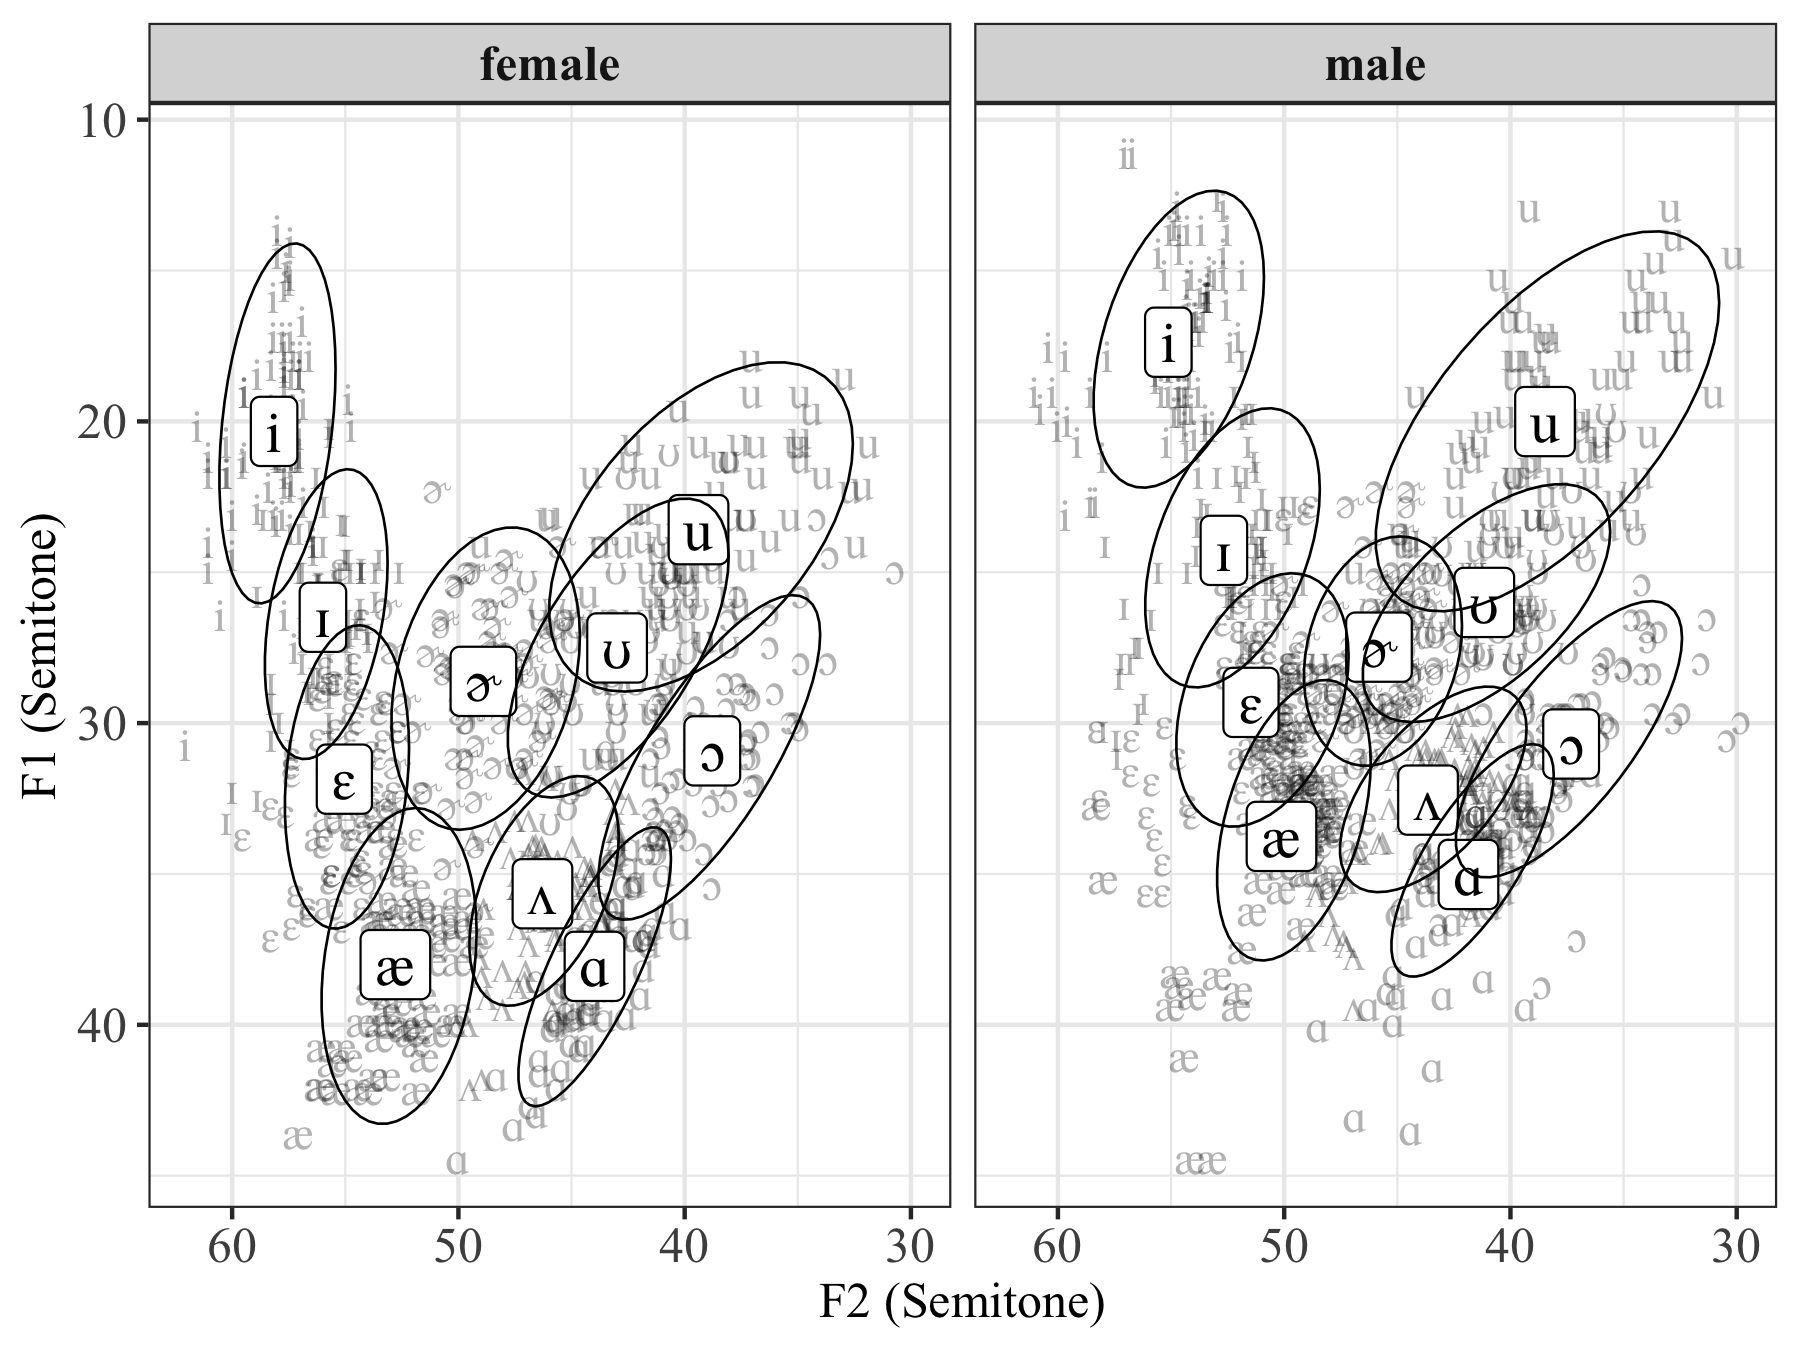
\includegraphics[width=0.6\linewidth]{figures/nativeVowel}
\caption{L1 Vowel Space (Peterson \& Barney, 1952)}
\end{figure}

\end{frame}

%---------------------------------------------
\begin{frame}
\frametitle{Background: Rationale}
\only<1>{
\begin{itemize} 
\item Does \textbf{Lexical Identification} play a role? \linebreak 
\end{itemize}
\begin{table}[]
\begin{tabular}{lll}
Pronunciation & Consonant Change & Vowel Change \\ 
\hline
{[ˈɜɹmi]}       & early            & army         \\
{[ˈɛltəmət]}    & estimate         & ultimate     \\
{[dɪ ˈzɔɹt]}    & resort           & dessert      \\
{[ˈkʰibrə]}     & zebra            & cobra       \\ 
\hline
\end{tabular}
\caption{Word Reconstruction Test (van Ooijen, 1996) }
\end{table}
\centering
{[ˈɜɹmi]}  --> Early or Army?

}
\only<2>{
\begin{itemize} 
\item Does \textbf{Lexical Identification} play a role? \linebreak 
\end{itemize}
\begin{table}[]
\begin{tabular}{lll}
Pronunciation & Consonant Change & \textbf{Vowel Change} \\ 
\hline
{[ˈɜɹmi]}       & early            & \textbf{army}         \\
{[ˈɛltəmət]}    & estimate     & \textbf{ultimate}     \\
{[dɪ ˈzɔɹt]}    & resort           & \textbf{dessert}      \\
{[ˈkʰibrə]}     & zebra            & \textbf{cobra}       \\ 
\hline
\end{tabular}
\caption{Word Reconstruction Test (van Ooijen, 1996) }
\end{table}
\begin{enumerate}
\item \textbf{Vowel Changes} are preferred (van Ooijen, 1996)  \linebreak$\rightarrow$Vowel changes are more tolerable ?
\item Vowel changes are less accented? 
\end{enumerate}
}

\end{frame}

%-------------------------------------

\begin{frame}
\frametitle{Background: Summary}

\begin{enumerate}
\onslide <1->{\item L1 speech exhibits variations (Dialectal and Contextual) \linebreak
			   (e.g., coda-deletion, /θ/$\rightarrow$/t/,  /faɪv/$\rightarrow$/faːv/) \linebreak
			   	-> Are they less accented?}\linebreak
\onslide <2->{\item Vowel changes are less likely to be perceived as a categorical change \linebreak
			-> Vowel changes could be less accented?}\linebreak
\onslide <3->{\item Consonants are more important in lexical identification.\linebreak
			-> Consonant changes could be more accented?}\linebreak
\onslide <4->{\item What about syllables?.\linebreak
			-> Deletion is less accented than epenthesis?}\linebreak
\end{enumerate}
\end{frame}
%---------------------------------------------
\section{Overview}
\begin{frame}
\frametitle{Overview}
\begin{enumerate}
\onslide <1->{\item Experiment 1: \linebreak
			   a pilot study, collecting accentedness ratings on 100 L2 stimuli} \linebreak
\onslide <2->{\item Experiment 2: \linebreak
			(1) added a training phase, controlled for intelligibility, (2) provided accentedness rankings, (3) hypothesized potential reasons for accentedness judgements}\linebreak
\onslide <3->{\item Experiment 3: \linebreak
			(1) modelled L1 phonetic/phonological knowledge, (2) investigated potential reasons for accentedness judgments }\linebreak

\end{enumerate}
\end{frame}

%--------------------------------------------
\section{Experiment 1}
\subsection{Task}
\begin{frame}
\frametitle{Experiment 1: Tasks}
\begin{enumerate}
\item{Design a perception study to obtain accentedness ratings;}\linebreak
\item{Rank the phonetic/phonological patterns by accentedness;}\linebreak
\end{enumerate}
\end{frame}
%-------------------------------------------

%------------------------------------------------
\subsection{Research Design}
\begin{frame}
\frametitle{Experiment 1: Stimuli Design}
Stimuli:
\begin{itemize} 
\item One potential “error” per stimulus 
\item A larger variety of  potential “errors”
\item No prosody manipulation 
\end{itemize}

\end{frame}
%------------------------------------------------
\begin{frame}
\frametitle{Experiment 1: Corpus}
Stimuli collection: \linebreak
Natural speech samples from the Speech Accent Achieve (Weinberger, 2019)
\begin{columns}[c] % The "c" option specifies centered vertical alignment while the "t" option is used for top vertical alignment
\column{.5\textwidth} % Left column and width
\begin{figure}
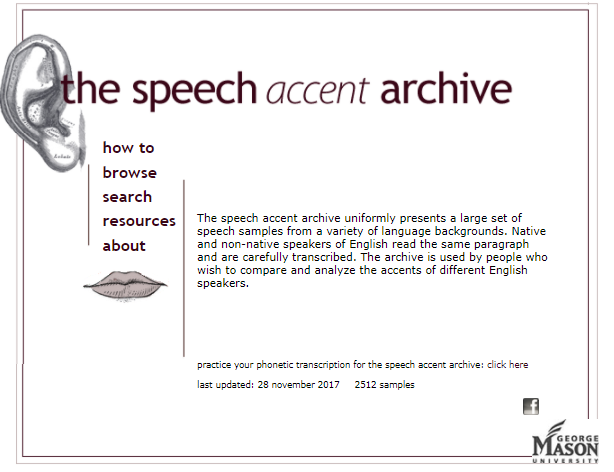
\includegraphics[width=0.8\linewidth]{figures/accent}
\linebreak \textsubscript{accent.gmu.edu}
\end{figure}
\column{.5\textwidth} % Right column and width
\begin{figure}
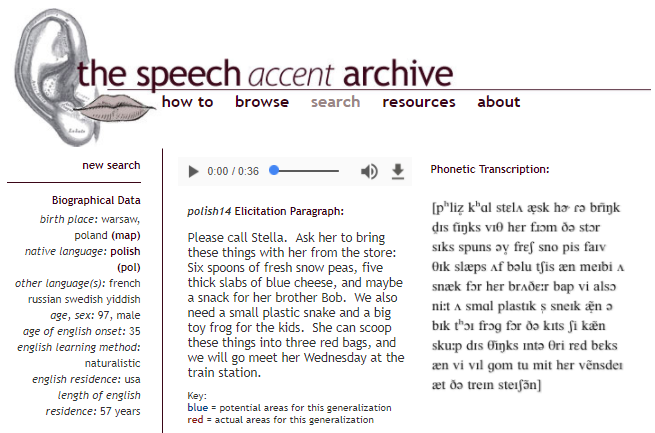
\includegraphics[width=0.8\linewidth]{figures/saademo}
%\linebreak \textsubscript{transcriber.accent.gmu.edu}
\end{figure}
\end{columns}
\end{frame}
%-----------------------------------------------

\begin{frame}
\frametitle{Experiment 1: Stimuli Classification}
Stimuli Classification:\linebreak
\begin{itemize}
\onslide<1->{\item \textbf{References:} The most common L1 productions ( L1 targets)\linebreak(e.g., [θɪk] for “thick”)} 

\onslide<2->{\item \textbf{Match}: L2 Stimuli that \textbf{match} the L1 targets (i.e., [θɪk])} \linebreak
\onslide<3->{\item \textbf{Mismatch}: L2 stimuli that \textbf{differ} from the L1 targets by \textbf{only one} element\linebreak
 \begin{enumerate}
     \item Consonant Mismatch (e.g., [tɪk])  \linebreak
     \item Vowel Mismatch (e.g., [θik])\linebreak
     \item Syllable Mismatch (e.g., [æskə]) \linebreak
   \end{enumerate}
}
\end{itemize}

\end{frame}
%--------------------------------
\begin{frame}
\frametitle{Experiment 1: Stimuli Examples}
Stimuli Illustration:\linebreak
\begin{table}[!h]
  \centering
  \caption{Types of Stimuli}
  \resizebox{0.9\textwidth}{!}{
    \begin{tabular}{p{5em}llll}
    \toprule
    Contexts & Match & Consonant & Vowel & Syllable \\
    \midrule
    please call &[pʰliz kʰɑl] &[{\color{red}p}liz kʰɑl]&[pʰliz kʰ{\color{red}o}l]&[pʰ{\color{red}ə}liz kʰɑl]\\
    ask her &[æsk (h)əɹ] &[æsk hə{\color{red}r}]&[{\color{red}ɑ}sk həɹ]&[æs{\color{red}\underline{ }} həɹ]\\
    six spoons &[sɪks spunz] &[sɪks spun{\color{red}ʃ}]&[s{\color{red}i}ks spunz]&[sɪks {\color{red}ə}spunz]\\
    five thick &[faɪv θɪk]&[faɪv {\color{red}t}ɪk] &[f{\color{red}a}v θɪk]&[faɪv{\color{red}ə} θɪk]\\
    small plastic &[smɑl pʰlæstɪk] &[smɑ{\color{red}ɭ} pʰlæstɪk]&[smɑl pʰlæst{\color{red}i}k]&[smɑl pʰlæs{\color{red}\underline{ }}ɪk]\\
    \bottomrule
    \end{tabular}%
   }
\end{table}%
\centering
All transcriptions were verified via acoustic analysis of the sound files
\end{frame}
%------------------------
\begin{frame}
\frametitle{Experiment 1: Prosody}
Control prosody in the least intrusive manner.  \linebreak
Prosody is a {\bf CONTROLLING} variable.  
\linebreak
\linebreak
Method: Dynamic Time Warping (DTW) 
\begin{itemize}
\item No acoustic manipulation required
\item Align F0 contours of two utterances
\item Produce a DTW score which represents alignment cost
\item The bigger the DTW score, bigger the intonational difference
\end{itemize}
\begin{columns}[c] % The "c" option specifies centered vertical alignment while the "t" option is used for top vertical alignment
\column{.45\textwidth} % Left column and width
\begin{figure}
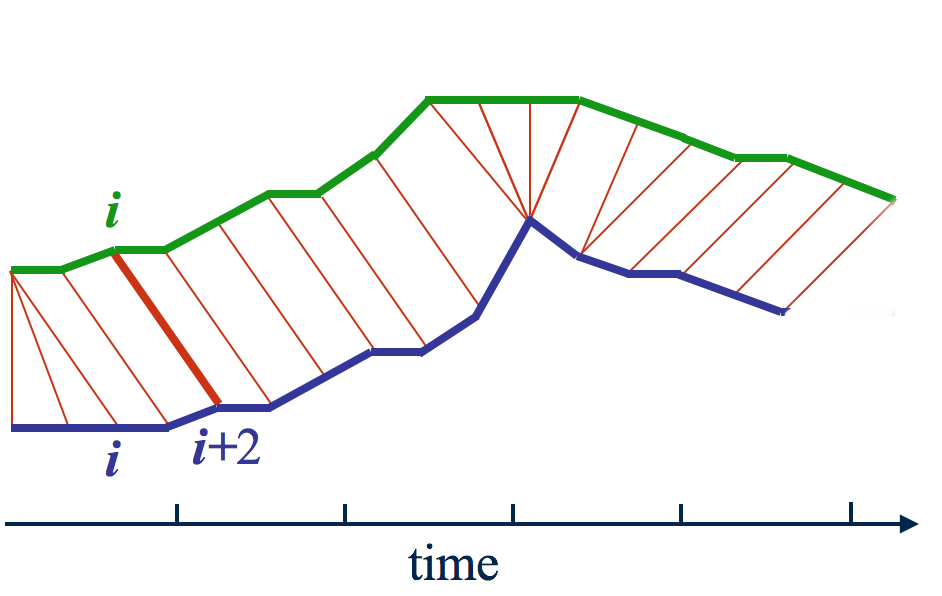
\includegraphics[width=0.8\linewidth]{figures/dtw1}
\linebreak \textsubscript{(Tsiporkova, 2007) }
\end{figure}
\column{.55\textwidth} % Right column and width
\begin{figure}
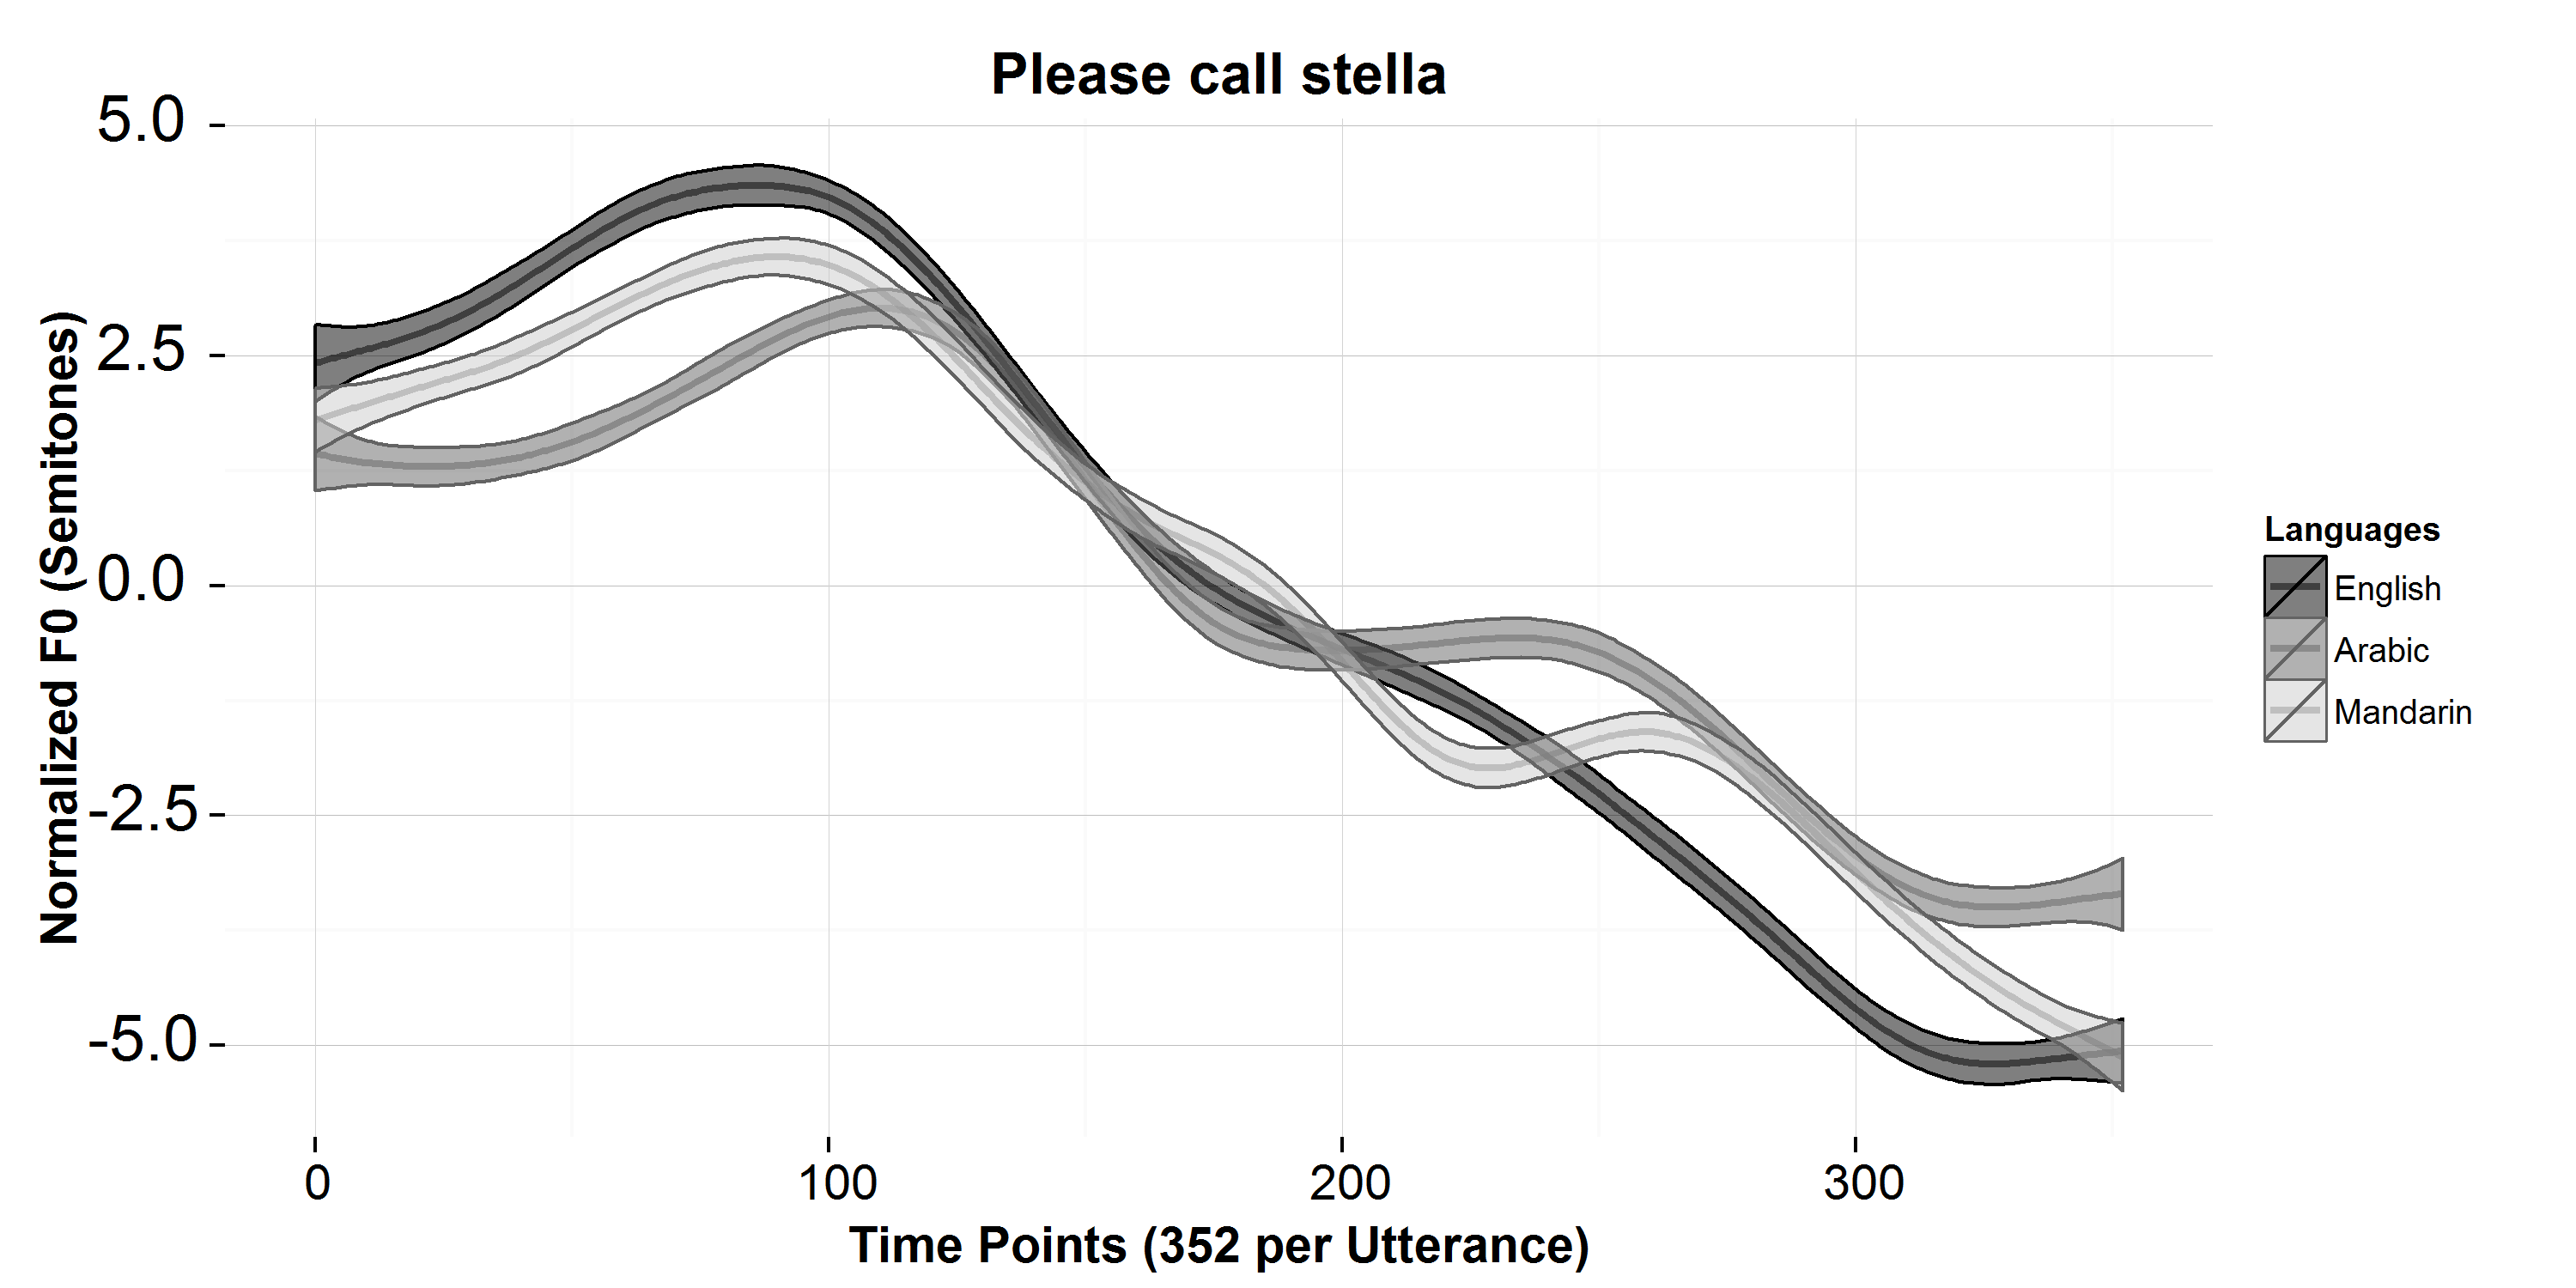
\includegraphics[width=0.9\linewidth]{figures/dtw2}
\linebreak\textsubscript{(Morrill \& Gao,2016)}
\end{figure}
\end{columns}
\end{frame}

%------------------------------------------------
\subsection{Interface}
\begin{frame}
\frametitle{Experiment 1: Procedure}
\begin{itemize}
\small{
\item Platform: Amazon Mechanical Turk 
\item Requirements for participants: US IPs, at least 95\%  acceptance rate.
\item Procedure:
}
\end{itemize}
\only <1>{
\begin{block}{Introduction}
\begin{figure}
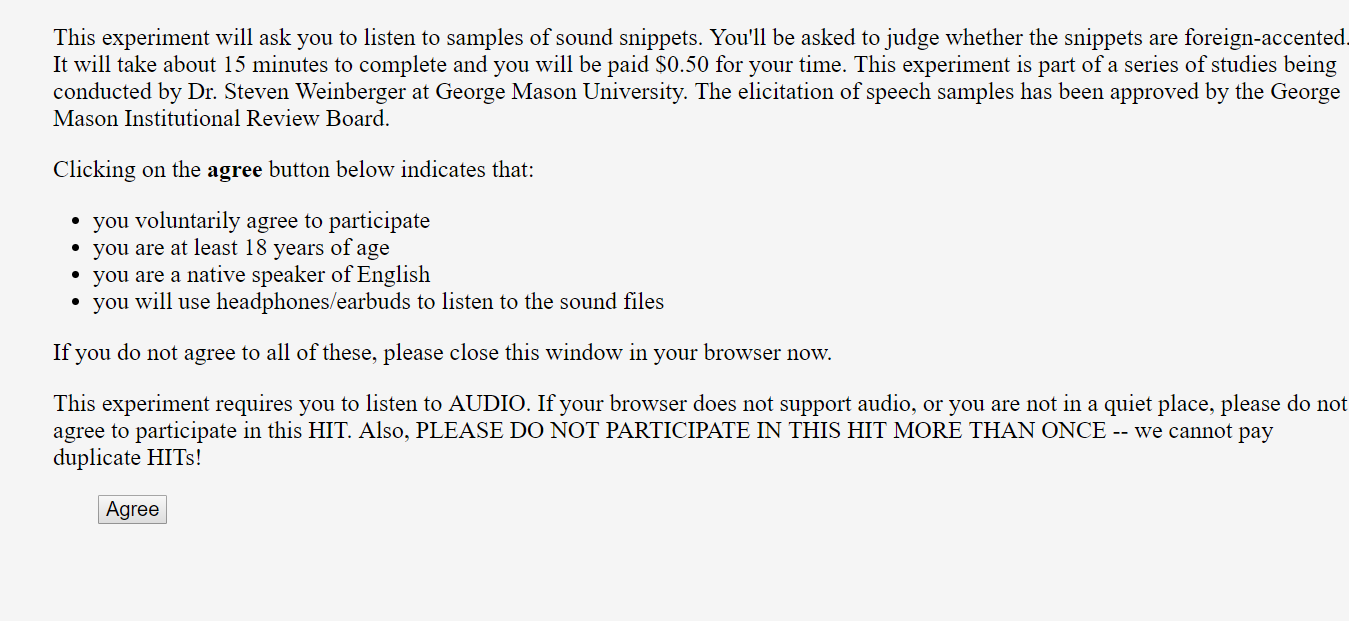
\includegraphics[width=0.8\linewidth]{figures/demo1}
\end{figure}
\end{block}}
\only <2>{
\begin{block}{Instruction}
\begin{figure}
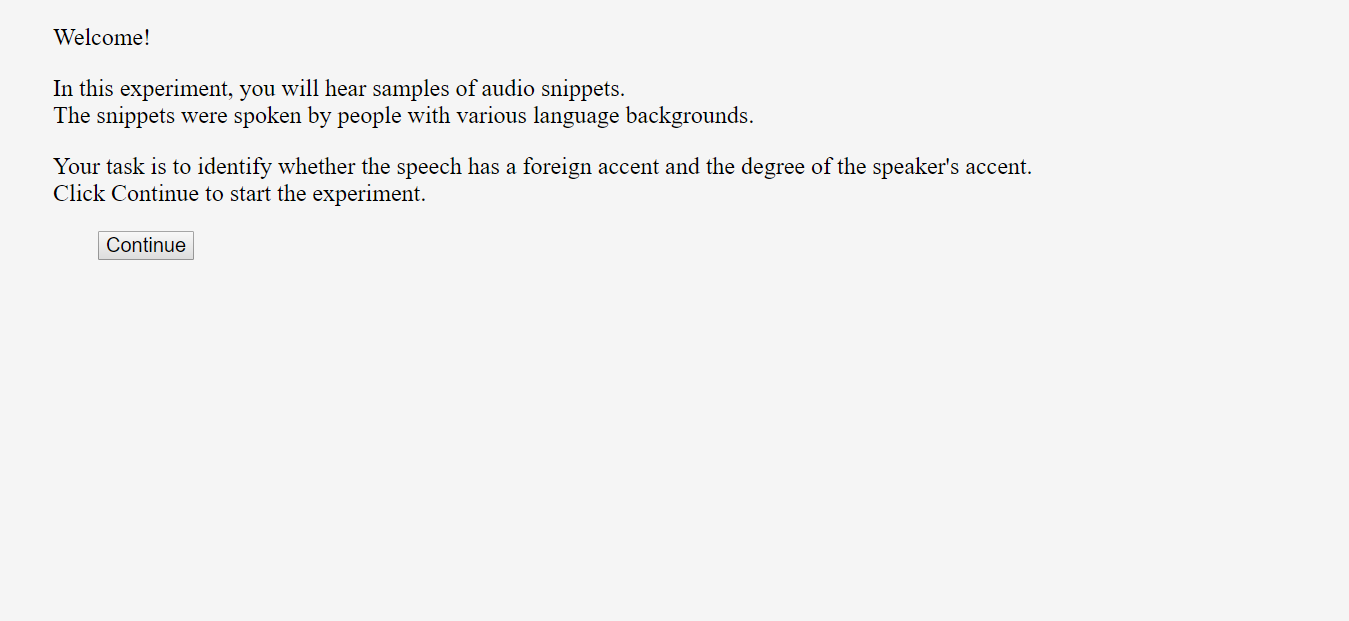
\includegraphics[width=0.8\linewidth]{figures/demo2}
\end{figure}
\end{block}}
\only <3>{
\begin{block}{Trials:Listen to snippets (Block Randomization)}
\begin{figure}
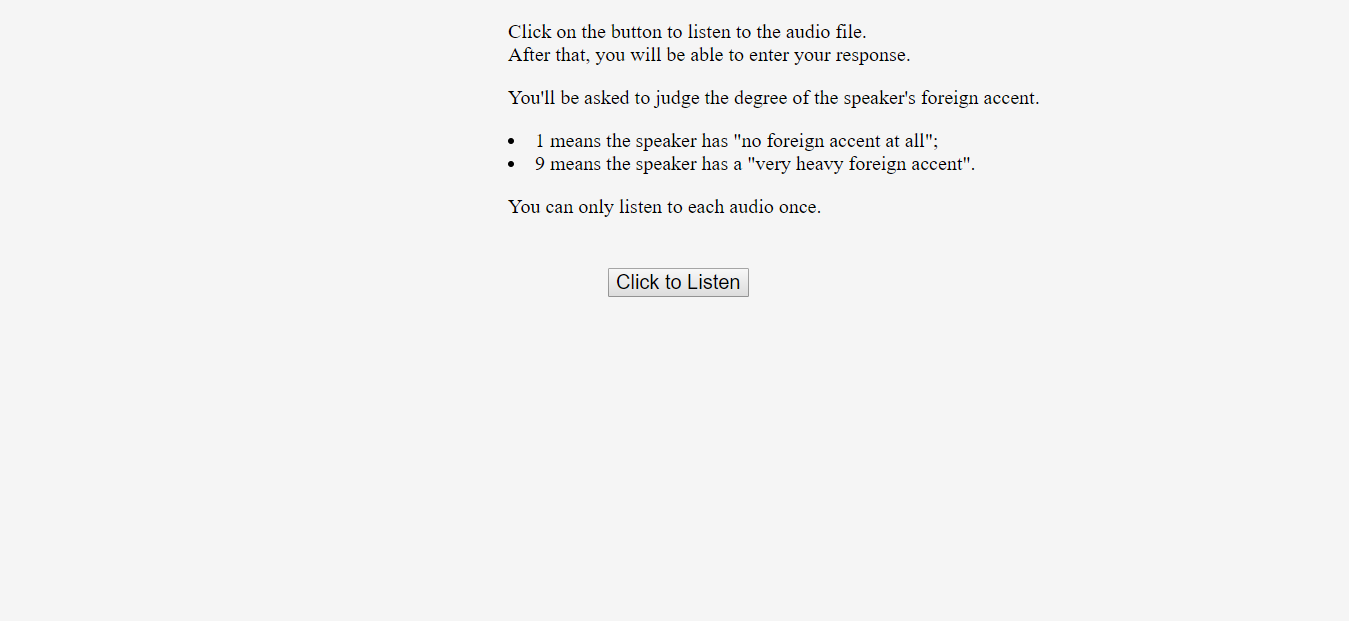
\includegraphics[width=0.8\linewidth]{figures/demo3}
\end{figure}
\end{block}}
\only <4>{
\begin{block}{Trials:Make accentedness judgment}
\begin{figure}
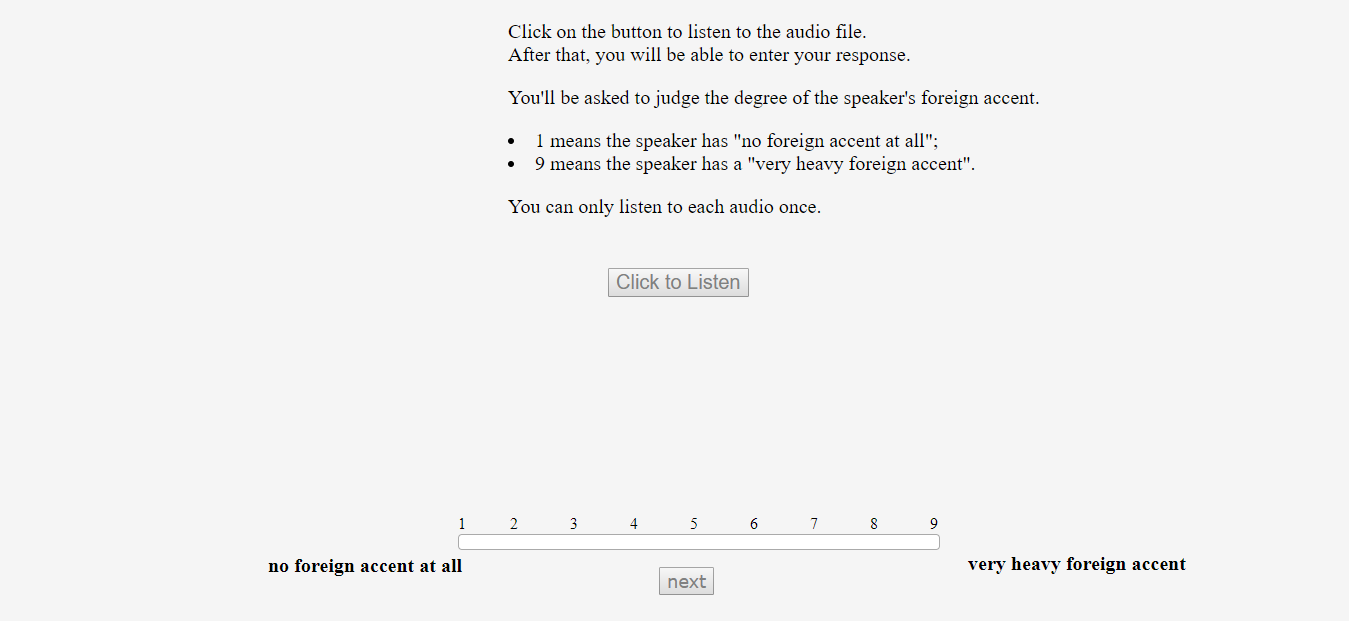
\includegraphics[width=0.8\linewidth]{figures/demo4}
\end{figure}
\end{block}}
\only <5>{
\begin{block}{Demographics}
\begin{figure}
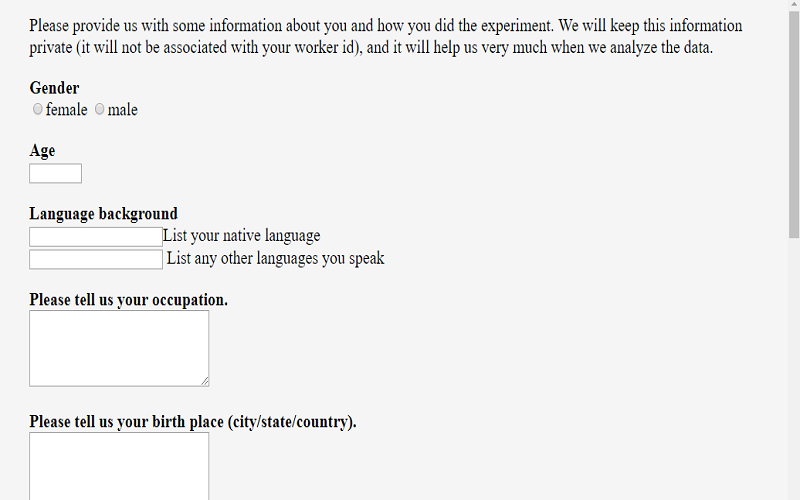
\includegraphics[width=0.8\linewidth]{figures/demo5}
\end{figure}
\end{block}}
\end{frame}

%------------------------------------------------
\subsection{Demos of raters}
\begin{frame}
\frametitle{Experiment 1: Rater Demographics}
\begin{itemize}
\item 108 Participants (L1 American English Speakers)\linebreak
\item {Male:61, Female:45, 2 did not report}\linebreak
\item {Age: range 20-66 (M=33.50, SD=12.51)}\linebreak
\item {Completion Time: M=12.33 min, SD=3.2 min; \linebreak Maximum time allowed:30 min}
\end{itemize}
\end{frame}
%------------------
\subsection{Results}
\begin{frame}
\frametitle{Experiment 1: Results}
\begin{block}{Meaning Ratings by Type}
\begin{center}
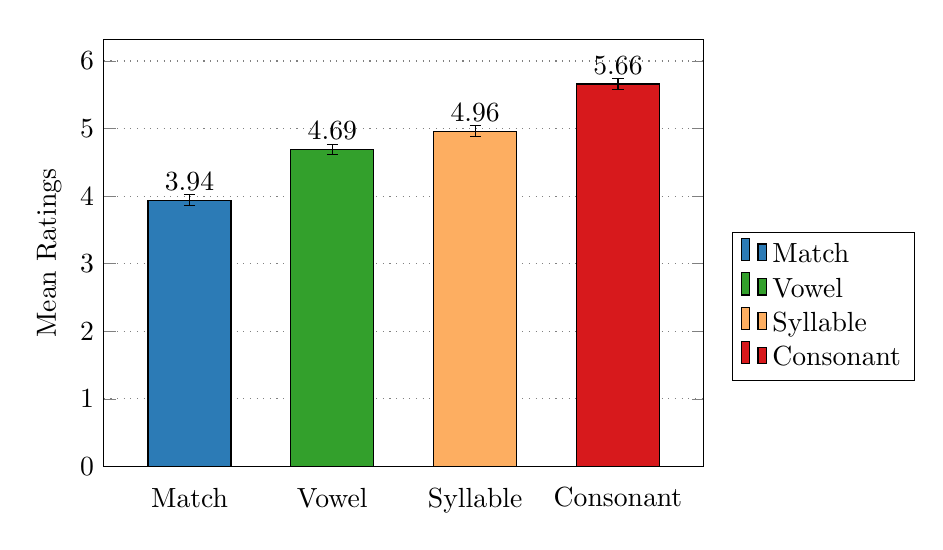
\begin{tikzpicture}
  \begin{axis}[
  ylabel={Mean Ratings},
width=9.2cm,
   height = 7cm,
    ytick distance=1,
        nodes near coords,
      major x tick style = transparent,
    ybar=3*\pgflinewidth,
      bar width=30pt,
      ymajorgrids = true,
      symbolic x coords={Match,Vowel,Syllable,Consonant},
      xtick ={Match,Vowel, Syllable, Consonant},
      scaled y ticks = false,
        legend style={at={(1.2,0.55)},
  anchor=north},
  legend cell align=left,
      enlarge x limits=0.20,
      ymin=0,
       every axis plot/.append style={
          ybar,
          bar shift=0pt,
          fill
        }
    ]
\addplot [fill=mycolor4,error bars/.cd, y dir=both, y explicit,error bar style=black] 
  coordinates {
          (Match, 3.94) += (0,0.08) -= (0,0.08)};
\addplot [fill=mycolor3,error bars/.cd, y dir=both, y explicit,error bar style=black] 
  coordinates {
          (Vowel, 4.69) += (0,0.08) -= (0,0.08)};
\addplot [fill=mycolor2,error bars/.cd, y dir=both, y explicit,error bar style=black] 
  coordinates {
          (Syllable, 4.96) += (0,0.08) -= (0,0.08)};
 \addplot [fill=mycolor1,error bars/.cd, y dir=both, y explicit,error bar style=black] 
  coordinates {
          (Consonant, 5.66) += (0,0.08) -= (0,0.08)};
 \legend{Match,Vowel,Syllable,Consonant}
 \end{axis}
\end{tikzpicture}
\end{center}


\end{block}
\end{frame}
%---------------------


\begin{frame}
\frametitle{Experiment 1: Ratings across Time}
\begin{center}
% Created by tikzDevice version 0.12.3 on 2019-11-24 19:33:25
% !TEX encoding = UTF-8 Unicode
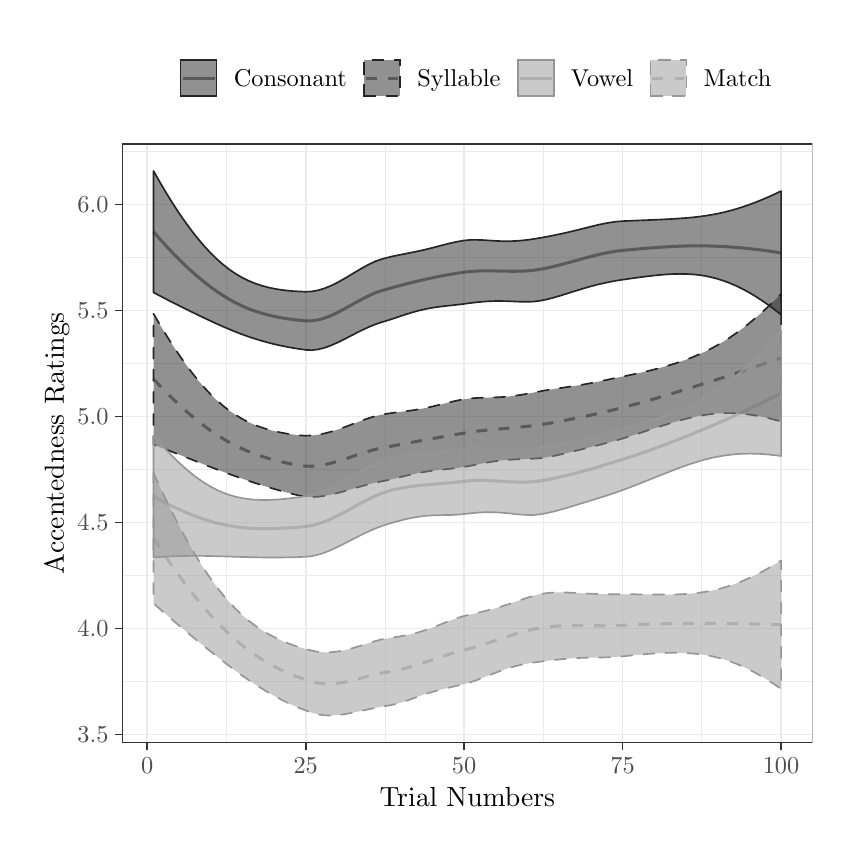
\begin{tikzpicture}[x=1pt,y=1pt]
\definecolor{fillColor}{RGB}{255,255,255}
\path[use as bounding box,fill=fillColor,fill opacity=0.00] (0,0) rectangle (289.08,289.08);
\begin{scope}
\path[clip] (  0.00,  0.00) rectangle (289.08,289.08);
\definecolor{drawColor}{RGB}{255,255,255}
\definecolor{fillColor}{RGB}{255,255,255}

\path[draw=drawColor,line width= 0.6pt,line join=round,line cap=round,fill=fillColor] (  0.00,  0.00) rectangle (289.08,289.08);
\end{scope}
\begin{scope}
\path[clip] ( 34.16, 30.69) rectangle (283.58,247.13);
\definecolor{fillColor}{RGB}{255,255,255}

\path[fill=fillColor] ( 34.16, 30.69) rectangle (283.58,247.13);
\definecolor{drawColor}{gray}{0.92}

\path[draw=drawColor,line width= 0.3pt,line join=round] ( 34.16, 52.87) --
	(283.58, 52.87);

\path[draw=drawColor,line width= 0.3pt,line join=round] ( 34.16, 91.17) --
	(283.58, 91.17);

\path[draw=drawColor,line width= 0.3pt,line join=round] ( 34.16,129.47) --
	(283.58,129.47);

\path[draw=drawColor,line width= 0.3pt,line join=round] ( 34.16,167.77) --
	(283.58,167.77);

\path[draw=drawColor,line width= 0.3pt,line join=round] ( 34.16,206.07) --
	(283.58,206.07);

\path[draw=drawColor,line width= 0.3pt,line join=round] ( 34.16,244.37) --
	(283.58,244.37);

\path[draw=drawColor,line width= 0.3pt,line join=round] ( 71.83, 30.69) --
	( 71.83,247.13);

\path[draw=drawColor,line width= 0.3pt,line join=round] (129.09, 30.69) --
	(129.09,247.13);

\path[draw=drawColor,line width= 0.3pt,line join=round] (186.35, 30.69) --
	(186.35,247.13);

\path[draw=drawColor,line width= 0.3pt,line join=round] (243.61, 30.69) --
	(243.61,247.13);

\path[draw=drawColor,line width= 0.6pt,line join=round] ( 34.16, 33.72) --
	(283.58, 33.72);

\path[draw=drawColor,line width= 0.6pt,line join=round] ( 34.16, 72.02) --
	(283.58, 72.02);

\path[draw=drawColor,line width= 0.6pt,line join=round] ( 34.16,110.32) --
	(283.58,110.32);

\path[draw=drawColor,line width= 0.6pt,line join=round] ( 34.16,148.62) --
	(283.58,148.62);

\path[draw=drawColor,line width= 0.6pt,line join=round] ( 34.16,186.92) --
	(283.58,186.92);

\path[draw=drawColor,line width= 0.6pt,line join=round] ( 34.16,225.22) --
	(283.58,225.22);

\path[draw=drawColor,line width= 0.6pt,line join=round] ( 43.20, 30.69) --
	( 43.20,247.13);

\path[draw=drawColor,line width= 0.6pt,line join=round] (100.46, 30.69) --
	(100.46,247.13);

\path[draw=drawColor,line width= 0.6pt,line join=round] (157.72, 30.69) --
	(157.72,247.13);

\path[draw=drawColor,line width= 0.6pt,line join=round] (214.98, 30.69) --
	(214.98,247.13);

\path[draw=drawColor,line width= 0.6pt,line join=round] (272.24, 30.69) --
	(272.24,247.13);
\definecolor{drawColor}{RGB}{37,37,37}

\path[draw=drawColor,draw opacity=0.50,line width= 1.1pt,line join=round] ( 45.49,215.33) --
	( 47.78,212.70) --
	( 50.07,210.17) --
	( 52.36,207.73) --
	( 54.66,205.39) --
	( 56.95,203.16) --
	( 59.24,201.04) --
	( 61.53,199.04) --
	( 63.82,197.15) --
	( 66.11,195.38) --
	( 68.40,193.73) --
	( 70.69,192.22) --
	( 72.98,190.83) --
	( 75.27,189.59) --
	( 77.56,188.49) --
	( 79.85,187.52) --
	( 82.14,186.67) --
	( 84.43,185.93) --
	( 86.72,185.30) --
	( 89.01,184.76) --
	( 91.30,184.31) --
	( 93.59,183.93) --
	( 95.88,183.62) --
	( 98.17,183.36) --
	(100.46,183.15) --
	(102.75,183.16) --
	(105.04,183.51) --
	(107.33,184.16) --
	(109.62,185.05) --
	(111.91,186.13) --
	(114.21,187.32) --
	(116.50,188.59) --
	(118.79,189.88) --
	(121.08,191.12) --
	(123.37,192.27) --
	(125.66,193.27) --
	(127.95,194.06) --
	(130.24,194.71) --
	(132.53,195.35) --
	(134.82,195.97) --
	(137.11,196.57) --
	(139.40,197.14) --
	(141.69,197.69) --
	(143.98,198.21) --
	(146.27,198.71) --
	(148.56,199.18) --
	(150.85,199.61) --
	(153.14,200.02) --
	(155.43,200.39) --
	(157.72,200.72) --
	(160.01,200.98) --
	(162.30,201.13) --
	(164.59,201.20) --
	(166.88,201.20) --
	(169.17,201.16) --
	(171.47,201.11) --
	(173.76,201.07) --
	(176.05,201.06) --
	(178.34,201.09) --
	(180.63,201.21) --
	(182.92,201.42) --
	(185.21,201.76) --
	(187.50,202.20) --
	(189.79,202.71) --
	(192.08,203.28) --
	(194.37,203.89) --
	(196.66,204.52) --
	(198.95,205.16) --
	(201.24,205.79) --
	(203.53,206.40) --
	(205.82,206.98) --
	(208.11,207.50) --
	(210.40,207.95) --
	(212.69,208.32) --
	(214.98,208.59) --
	(217.27,208.80) --
	(219.56,209.01) --
	(221.85,209.22) --
	(224.14,209.41) --
	(226.43,209.59) --
	(228.73,209.75) --
	(231.02,209.89) --
	(233.31,210.02) --
	(235.60,210.12) --
	(237.89,210.19) --
	(240.18,210.24) --
	(242.47,210.25) --
	(244.76,210.23) --
	(247.05,210.17) --
	(249.34,210.09) --
	(251.63,209.97) --
	(253.92,209.83) --
	(256.21,209.65) --
	(258.50,209.45) --
	(260.79,209.22) --
	(263.08,208.97) --
	(265.37,208.68) --
	(267.66,208.38) --
	(269.95,208.05) --
	(272.24,207.70);

\path[draw=drawColor,draw opacity=0.50,line width= 1.1pt,dash pattern=on 4pt off 4pt ,line join=round] ( 45.49,162.06) --
	( 47.78,159.65) --
	( 50.07,157.31) --
	( 52.36,155.05) --
	( 54.66,152.87) --
	( 56.95,150.79) --
	( 59.24,148.80) --
	( 61.53,146.91) --
	( 63.82,145.13) --
	( 66.11,143.46) --
	( 68.40,141.91) --
	( 70.69,140.48) --
	( 72.98,139.17) --
	( 75.27,137.98) --
	( 77.56,136.90) --
	( 79.85,135.92) --
	( 82.14,135.03) --
	( 84.43,134.23) --
	( 86.72,133.51) --
	( 89.01,132.86) --
	( 91.30,132.28) --
	( 93.59,131.76) --
	( 95.88,131.30) --
	( 98.17,130.88) --
	(100.46,130.62) --
	(102.75,130.60) --
	(105.04,130.80) --
	(107.33,131.18) --
	(109.62,131.71) --
	(111.91,132.35) --
	(114.21,133.07) --
	(116.50,133.84) --
	(118.79,134.62) --
	(121.08,135.38) --
	(123.37,136.08) --
	(125.66,136.70) --
	(127.95,137.20) --
	(130.24,137.63) --
	(132.53,138.05) --
	(134.82,138.48) --
	(137.11,138.91) --
	(139.40,139.33) --
	(141.69,139.75) --
	(143.98,140.17) --
	(146.27,140.59) --
	(148.56,141.00) --
	(150.85,141.40) --
	(153.14,141.80) --
	(155.43,142.20) --
	(157.72,142.59) --
	(160.01,142.94) --
	(162.30,143.25) --
	(164.59,143.52) --
	(166.88,143.76) --
	(169.17,143.97) --
	(171.47,144.17) --
	(173.76,144.37) --
	(176.05,144.57) --
	(178.34,144.79) --
	(180.63,145.03) --
	(182.92,145.30) --
	(185.21,145.60) --
	(187.50,145.96) --
	(189.79,146.36) --
	(192.08,146.77) --
	(194.37,147.20) --
	(196.66,147.65) --
	(198.95,148.11) --
	(201.24,148.59) --
	(203.53,149.09) --
	(205.82,149.61) --
	(208.11,150.13) --
	(210.40,150.68) --
	(212.69,151.24) --
	(214.98,151.81) --
	(217.27,152.40) --
	(219.56,153.01) --
	(221.85,153.64) --
	(224.14,154.29) --
	(226.43,154.95) --
	(228.73,155.62) --
	(231.02,156.31) --
	(233.31,157.01) --
	(235.60,157.71) --
	(237.89,158.42) --
	(240.18,159.14) --
	(242.47,159.86) --
	(244.76,160.58) --
	(247.05,161.30) --
	(249.34,162.03) --
	(251.63,162.77) --
	(253.92,163.51) --
	(256.21,164.27) --
	(258.50,165.03) --
	(260.79,165.80) --
	(263.08,166.58) --
	(265.37,167.37) --
	(267.66,168.17) --
	(269.95,168.98) --
	(272.24,169.81);
\definecolor{drawColor}{RGB}{150,150,150}

\path[draw=drawColor,draw opacity=0.50,line width= 1.1pt,line join=round] ( 45.49,119.69) --
	( 47.78,118.44) --
	( 50.07,117.24) --
	( 52.36,116.10) --
	( 54.66,115.03) --
	( 56.95,114.02) --
	( 59.24,113.07) --
	( 61.53,112.20) --
	( 63.82,111.41) --
	( 66.11,110.69) --
	( 68.40,110.07) --
	( 70.69,109.53) --
	( 72.98,109.08) --
	( 75.27,108.72) --
	( 77.56,108.44) --
	( 79.85,108.24) --
	( 82.14,108.10) --
	( 84.43,108.03) --
	( 86.72,108.02) --
	( 89.01,108.06) --
	( 91.30,108.15) --
	( 93.59,108.28) --
	( 95.88,108.43) --
	( 98.17,108.62) --
	(100.46,108.83) --
	(102.75,109.18) --
	(105.04,109.78) --
	(107.33,110.58) --
	(109.62,111.56) --
	(111.91,112.66) --
	(114.21,113.86) --
	(116.50,115.11) --
	(118.79,116.38) --
	(121.08,117.62) --
	(123.37,118.80) --
	(125.66,119.88) --
	(127.95,120.83) --
	(130.24,121.59) --
	(132.53,122.19) --
	(134.82,122.69) --
	(137.11,123.09) --
	(139.40,123.42) --
	(141.69,123.69) --
	(143.98,123.91) --
	(146.27,124.10) --
	(148.56,124.28) --
	(150.85,124.46) --
	(153.14,124.66) --
	(155.43,124.89) --
	(157.72,125.16) --
	(160.01,125.40) --
	(162.30,125.50) --
	(164.59,125.50) --
	(166.88,125.42) --
	(169.17,125.30) --
	(171.47,125.15) --
	(173.76,125.01) --
	(176.05,124.90) --
	(178.34,124.85) --
	(180.63,124.88) --
	(182.92,125.03) --
	(185.21,125.32) --
	(187.50,125.71) --
	(189.79,126.15) --
	(192.08,126.64) --
	(194.37,127.16) --
	(196.66,127.73) --
	(198.95,128.32) --
	(201.24,128.95) --
	(203.53,129.60) --
	(205.82,130.27) --
	(208.11,130.96) --
	(210.40,131.67) --
	(212.69,132.38) --
	(214.98,133.10) --
	(217.27,133.83) --
	(219.56,134.58) --
	(221.85,135.36) --
	(224.14,136.16) --
	(226.43,136.97) --
	(228.73,137.81) --
	(231.02,138.67) --
	(233.31,139.55) --
	(235.60,140.45) --
	(237.89,141.36) --
	(240.18,142.29) --
	(242.47,143.23) --
	(244.76,144.19) --
	(247.05,145.16) --
	(249.34,146.15) --
	(251.63,147.15) --
	(253.92,148.17) --
	(256.21,149.21) --
	(258.50,150.27) --
	(260.79,151.35) --
	(263.08,152.44) --
	(265.37,153.55) --
	(267.66,154.68) --
	(269.95,155.83) --
	(272.24,157.00);

\path[draw=drawColor,draw opacity=0.50,line width= 1.1pt,dash pattern=on 4pt off 4pt ,line join=round] ( 45.49,104.65) --
	( 47.78,101.10) --
	( 50.07, 97.66) --
	( 52.36, 94.32) --
	( 54.66, 91.11) --
	( 56.95, 88.01) --
	( 59.24, 85.03) --
	( 61.53, 82.17) --
	( 63.82, 79.44) --
	( 66.11, 76.83) --
	( 68.40, 74.36) --
	( 70.69, 72.02) --
	( 72.98, 69.82) --
	( 75.27, 67.76) --
	( 77.56, 65.85) --
	( 79.85, 64.08) --
	( 82.14, 62.44) --
	( 84.43, 60.94) --
	( 86.72, 59.55) --
	( 89.01, 58.28) --
	( 91.30, 57.12) --
	( 93.59, 56.06) --
	( 95.88, 55.10) --
	( 98.17, 54.23) --
	(100.46, 53.45) --
	(102.75, 52.74) --
	(105.04, 52.21) --
	(107.33, 51.97) --
	(109.62, 51.96) --
	(111.91, 52.16) --
	(114.21, 52.51) --
	(116.50, 52.99) --
	(118.79, 53.56) --
	(121.08, 54.16) --
	(123.37, 54.78) --
	(125.66, 55.36) --
	(127.95, 55.88) --
	(130.24, 56.28) --
	(132.53, 56.68) --
	(134.82, 57.18) --
	(137.11, 57.78) --
	(139.40, 58.44) --
	(141.69, 59.16) --
	(143.98, 59.91) --
	(146.27, 60.68) --
	(148.56, 61.45) --
	(150.85, 62.21) --
	(153.14, 62.93) --
	(155.43, 63.59) --
	(157.72, 64.19) --
	(160.01, 64.79) --
	(162.30, 65.45) --
	(164.59, 66.16) --
	(166.88, 66.91) --
	(169.17, 67.68) --
	(171.47, 68.44) --
	(173.76, 69.20) --
	(176.05, 69.92) --
	(178.34, 70.60) --
	(180.63, 71.21) --
	(182.92, 71.75) --
	(185.21, 72.19) --
	(187.50, 72.52) --
	(189.79, 72.75) --
	(192.08, 72.90) --
	(194.37, 72.99) --
	(196.66, 73.03) --
	(198.95, 73.04) --
	(201.24, 73.02) --
	(203.53, 72.99) --
	(205.82, 72.96) --
	(208.11, 72.95) --
	(210.40, 72.96) --
	(212.69, 73.01) --
	(214.98, 73.11) --
	(217.27, 73.24) --
	(219.56, 73.35) --
	(221.85, 73.44) --
	(224.14, 73.52) --
	(226.43, 73.59) --
	(228.73, 73.65) --
	(231.02, 73.69) --
	(233.31, 73.73) --
	(235.60, 73.76) --
	(237.89, 73.78) --
	(240.18, 73.79) --
	(242.47, 73.80) --
	(244.76, 73.80) --
	(247.05, 73.80) --
	(249.34, 73.79) --
	(251.63, 73.78) --
	(253.92, 73.76) --
	(256.21, 73.74) --
	(258.50, 73.70) --
	(260.79, 73.66) --
	(263.08, 73.61) --
	(265.37, 73.55) --
	(267.66, 73.48) --
	(269.95, 73.41) --
	(272.24, 73.32);
\definecolor{drawColor}{RGB}{37,37,37}
\definecolor{fillColor}{RGB}{37,37,37}

\path[draw=drawColor,line width= 0.6pt,line join=round,line cap=round,fill=fillColor,fill opacity=0.50] ( 45.49,237.29) --
	( 47.78,233.24) --
	( 50.07,229.36) --
	( 52.36,225.67) --
	( 54.66,222.15) --
	( 56.95,218.84) --
	( 59.24,215.72) --
	( 61.53,212.82) --
	( 63.82,210.13) --
	( 66.11,207.66) --
	( 68.40,205.42) --
	( 70.69,203.41) --
	( 72.98,201.63) --
	( 75.27,200.08) --
	( 77.56,198.74) --
	( 79.85,197.62) --
	( 82.14,196.68) --
	( 84.43,195.90) --
	( 86.72,195.27) --
	( 89.01,194.77) --
	( 91.30,194.39) --
	( 93.59,194.10) --
	( 95.88,193.89) --
	( 98.17,193.75) --
	(100.46,193.66) --
	(102.75,193.77) --
	(105.04,194.20) --
	(107.33,194.91) --
	(109.62,195.85) --
	(111.91,196.98) --
	(114.21,198.26) --
	(116.50,199.61) --
	(118.79,201.00) --
	(121.08,202.34) --
	(123.37,203.58) --
	(125.66,204.65) --
	(127.95,205.46) --
	(130.24,206.07) --
	(132.53,206.60) --
	(134.82,207.06) --
	(137.11,207.51) --
	(139.40,207.96) --
	(141.69,208.45) --
	(143.98,208.97) --
	(146.27,209.54) --
	(148.56,210.14) --
	(150.85,210.74) --
	(153.14,211.30) --
	(155.43,211.79) --
	(157.72,212.18) --
	(160.01,212.39) --
	(162.30,212.41) --
	(164.59,212.32) --
	(166.88,212.18) --
	(169.17,212.03) --
	(171.47,211.93) --
	(173.76,211.91) --
	(176.05,211.99) --
	(178.34,212.15) --
	(180.63,212.41) --
	(182.92,212.73) --
	(185.21,213.12) --
	(187.50,213.53) --
	(189.79,213.98) --
	(192.08,214.45) --
	(194.37,214.95) --
	(196.66,215.49) --
	(198.95,216.05) --
	(201.24,216.62) --
	(203.53,217.19) --
	(205.82,217.75) --
	(208.11,218.25) --
	(210.40,218.67) --
	(212.69,218.99) --
	(214.98,219.17) --
	(217.27,219.27) --
	(219.56,219.37) --
	(221.85,219.46) --
	(224.14,219.55) --
	(226.43,219.65) --
	(228.73,219.75) --
	(231.02,219.86) --
	(233.31,219.99) --
	(235.60,220.14) --
	(237.89,220.31) --
	(240.18,220.52) --
	(242.47,220.78) --
	(244.76,221.08) --
	(247.05,221.45) --
	(249.34,221.89) --
	(251.63,222.39) --
	(253.92,222.97) --
	(256.21,223.62) --
	(258.50,224.35) --
	(260.79,225.14) --
	(263.08,226.00) --
	(265.37,226.92) --
	(267.66,227.90) --
	(269.95,228.94) --
	(272.24,230.04) --
	(272.24,185.36) --
	(269.95,187.16) --
	(267.66,188.86) --
	(265.37,190.45) --
	(263.08,191.94) --
	(260.79,193.31) --
	(258.50,194.56) --
	(256.21,195.69) --
	(253.92,196.69) --
	(251.63,197.56) --
	(249.34,198.29) --
	(247.05,198.90) --
	(244.76,199.37) --
	(242.47,199.72) --
	(240.18,199.95) --
	(237.89,200.07) --
	(235.60,200.10) --
	(233.31,200.05) --
	(231.02,199.93) --
	(228.73,199.75) --
	(226.43,199.52) --
	(224.14,199.26) --
	(221.85,198.97) --
	(219.56,198.66) --
	(217.27,198.34) --
	(214.98,198.01) --
	(212.69,197.65) --
	(210.40,197.23) --
	(208.11,196.74) --
	(205.82,196.21) --
	(203.53,195.61) --
	(201.24,194.96) --
	(198.95,194.27) --
	(196.66,193.55) --
	(194.37,192.83) --
	(192.08,192.11) --
	(189.79,191.45) --
	(187.50,190.87) --
	(185.21,190.40) --
	(182.92,190.11) --
	(180.63,190.01) --
	(178.34,190.03) --
	(176.05,190.13) --
	(173.76,190.23) --
	(171.47,190.29) --
	(169.17,190.30) --
	(166.88,190.22) --
	(164.59,190.07) --
	(162.30,189.85) --
	(160.01,189.58) --
	(157.72,189.27) --
	(155.43,188.98) --
	(153.14,188.73) --
	(150.85,188.49) --
	(148.56,188.21) --
	(146.27,187.87) --
	(143.98,187.45) --
	(141.69,186.93) --
	(139.40,186.32) --
	(137.11,185.62) --
	(134.82,184.87) --
	(132.53,184.10) --
	(130.24,183.35) --
	(127.95,182.65) --
	(125.66,181.89) --
	(123.37,180.96) --
	(121.08,179.90) --
	(118.79,178.76) --
	(116.50,177.57) --
	(114.21,176.39) --
	(111.91,175.27) --
	(109.62,174.25) --
	(107.33,173.42) --
	(105.04,172.83) --
	(102.75,172.54) --
	(100.46,172.64) --
	( 98.17,172.97) --
	( 95.88,173.34) --
	( 93.59,173.75) --
	( 91.30,174.22) --
	( 89.01,174.74) --
	( 86.72,175.32) --
	( 84.43,175.96) --
	( 82.14,176.66) --
	( 79.85,177.41) --
	( 77.56,178.23) --
	( 75.27,179.10) --
	( 72.98,180.04) --
	( 70.69,181.02) --
	( 68.40,182.04) --
	( 66.11,183.09) --
	( 63.82,184.16) --
	( 61.53,185.26) --
	( 59.24,186.37) --
	( 56.95,187.49) --
	( 54.66,188.64) --
	( 52.36,189.80) --
	( 50.07,190.97) --
	( 47.78,192.17) --
	( 45.49,193.38) --
	cycle;

\path[draw=drawColor,line width= 0.6pt,dash pattern=on 4pt off 4pt ,line join=round,line cap=round,fill=fillColor,fill opacity=0.50] ( 45.49,185.70) --
	( 47.78,181.77) --
	( 50.07,177.99) --
	( 52.36,174.37) --
	( 54.66,170.92) --
	( 56.95,167.65) --
	( 59.24,164.57) --
	( 61.53,161.70) --
	( 63.82,159.03) --
	( 66.11,156.59) --
	( 68.40,154.37) --
	( 70.69,152.37) --
	( 72.98,150.61) --
	( 75.27,149.05) --
	( 77.56,147.69) --
	( 79.85,146.51) --
	( 82.14,145.50) --
	( 84.43,144.64) --
	( 86.72,143.92) --
	( 89.01,143.31) --
	( 91.30,142.81) --
	( 93.59,142.39) --
	( 95.88,142.05) --
	( 98.17,141.77) --
	(100.46,141.63) --
	(102.75,141.72) --
	(105.04,142.01) --
	(107.33,142.47) --
	(109.62,143.08) --
	(111.91,143.81) --
	(114.21,144.62) --
	(116.50,145.49) --
	(118.79,146.37) --
	(121.08,147.24) --
	(123.37,148.03) --
	(125.66,148.72) --
	(127.95,149.25) --
	(130.24,149.64) --
	(132.53,149.96) --
	(134.82,150.25) --
	(137.11,150.55) --
	(139.40,150.87) --
	(141.69,151.25) --
	(143.98,151.69) --
	(146.27,152.19) --
	(148.56,152.75) --
	(150.85,153.32) --
	(153.14,153.88) --
	(155.43,154.39) --
	(157.72,154.82) --
	(160.01,155.11) --
	(162.30,155.28) --
	(164.59,155.37) --
	(166.88,155.43) --
	(169.17,155.50) --
	(171.47,155.61) --
	(173.76,155.80) --
	(176.05,156.07) --
	(178.34,156.41) --
	(180.63,156.81) --
	(182.92,157.25) --
	(185.21,157.68) --
	(187.50,158.09) --
	(189.79,158.46) --
	(192.08,158.80) --
	(194.37,159.13) --
	(196.66,159.46) --
	(198.95,159.82) --
	(201.24,160.21) --
	(203.53,160.63) --
	(205.82,161.08) --
	(208.11,161.56) --
	(210.40,162.05) --
	(212.69,162.54) --
	(214.98,163.01) --
	(217.27,163.48) --
	(219.56,163.97) --
	(221.85,164.48) --
	(224.14,165.02) --
	(226.43,165.59) --
	(228.73,166.20) --
	(231.02,166.85) --
	(233.31,167.54) --
	(235.60,168.29) --
	(237.89,169.11) --
	(240.18,169.99) --
	(242.47,170.95) --
	(244.76,172.00) --
	(247.05,173.15) --
	(249.34,174.40) --
	(251.63,175.76) --
	(253.92,177.23) --
	(256.21,178.82) --
	(258.50,180.51) --
	(260.79,182.32) --
	(263.08,184.23) --
	(265.37,186.25) --
	(267.66,188.36) --
	(269.95,190.57) --
	(272.24,192.87) --
	(272.24,146.75) --
	(269.95,147.40) --
	(267.66,147.98) --
	(265.37,148.49) --
	(263.08,148.92) --
	(260.79,149.27) --
	(258.50,149.54) --
	(256.21,149.71) --
	(253.92,149.79) --
	(251.63,149.78) --
	(249.34,149.67) --
	(247.05,149.46) --
	(244.76,149.15) --
	(242.47,148.76) --
	(240.18,148.28) --
	(237.89,147.74) --
	(235.60,147.13) --
	(233.31,146.47) --
	(231.02,145.77) --
	(228.73,145.05) --
	(226.43,144.31) --
	(224.14,143.56) --
	(221.85,142.80) --
	(219.56,142.06) --
	(217.27,141.33) --
	(214.98,140.61) --
	(212.69,139.94) --
	(210.40,139.31) --
	(208.11,138.71) --
	(205.82,138.13) --
	(203.53,137.55) --
	(201.24,136.98) --
	(198.95,136.41) --
	(196.66,135.84) --
	(194.37,135.28) --
	(192.08,134.74) --
	(189.79,134.26) --
	(187.50,133.83) --
	(185.21,133.53) --
	(182.92,133.34) --
	(180.63,133.24) --
	(178.34,133.16) --
	(176.05,133.08) --
	(173.76,132.94) --
	(171.47,132.73) --
	(169.17,132.45) --
	(166.88,132.09) --
	(164.59,131.67) --
	(162.30,131.22) --
	(160.01,130.78) --
	(157.72,130.36) --
	(155.43,130.01) --
	(153.14,129.73) --
	(150.85,129.49) --
	(148.56,129.25) --
	(146.27,128.98) --
	(143.98,128.65) --
	(141.69,128.26) --
	(139.40,127.79) --
	(137.11,127.27) --
	(134.82,126.71) --
	(132.53,126.14) --
	(130.24,125.61) --
	(127.95,125.15) --
	(125.66,124.68) --
	(123.37,124.13) --
	(121.08,123.51) --
	(118.79,122.86) --
	(116.50,122.18) --
	(114.21,121.52) --
	(111.91,120.89) --
	(109.62,120.34) --
	(107.33,119.89) --
	(105.04,119.59) --
	(102.75,119.48) --
	(100.46,119.60) --
	( 98.17,119.99) --
	( 95.88,120.54) --
	( 93.59,121.13) --
	( 91.30,121.75) --
	( 89.01,122.41) --
	( 86.72,123.10) --
	( 84.43,123.81) --
	( 82.14,124.56) --
	( 79.85,125.32) --
	( 77.56,126.11) --
	( 75.27,126.92) --
	( 72.98,127.74) --
	( 70.69,128.58) --
	( 68.40,129.45) --
	( 66.11,130.33) --
	( 63.82,131.22) --
	( 61.53,132.12) --
	( 59.24,133.02) --
	( 56.95,133.93) --
	( 54.66,134.83) --
	( 52.36,135.73) --
	( 50.07,136.63) --
	( 47.78,137.52) --
	( 45.49,138.41) --
	cycle;
\definecolor{drawColor}{gray}{0.59}
\definecolor{fillColor}{RGB}{150,150,150}

\path[draw=drawColor,line width= 0.6pt,line join=round,line cap=round,fill=fillColor,fill opacity=0.50] ( 45.49,141.72) --
	( 47.78,139.07) --
	( 50.07,136.54) --
	( 52.36,134.16) --
	( 54.66,131.92) --
	( 56.95,129.84) --
	( 59.24,127.92) --
	( 61.53,126.18) --
	( 63.82,124.61) --
	( 66.11,123.23) --
	( 68.40,122.03) --
	( 70.69,121.02) --
	( 72.98,120.20) --
	( 75.27,119.55) --
	( 77.56,119.06) --
	( 79.85,118.72) --
	( 82.14,118.51) --
	( 84.43,118.41) --
	( 86.72,118.41) --
	( 89.01,118.50) --
	( 91.30,118.66) --
	( 93.59,118.88) --
	( 95.88,119.15) --
	( 98.17,119.45) --
	(100.46,119.78) --
	(102.75,120.23) --
	(105.04,120.90) --
	(107.33,121.76) --
	(109.62,122.78) --
	(111.91,123.93) --
	(114.21,125.18) --
	(116.50,126.51) --
	(118.79,127.86) --
	(121.08,129.20) --
	(123.37,130.48) --
	(125.66,131.65) --
	(127.95,132.65) --
	(130.24,133.43) --
	(132.53,133.98) --
	(134.82,134.35) --
	(137.11,134.60) --
	(139.40,134.78) --
	(141.69,134.95) --
	(143.98,135.13) --
	(146.27,135.36) --
	(148.56,135.64) --
	(150.85,135.96) --
	(153.14,136.32) --
	(155.43,136.67) --
	(157.72,137.00) --
	(160.01,137.19) --
	(162.30,137.19) --
	(164.59,137.05) --
	(166.88,136.85) --
	(169.17,136.65) --
	(171.47,136.50) --
	(173.76,136.42) --
	(176.05,136.45) --
	(178.34,136.57) --
	(180.63,136.78) --
	(182.92,137.07) --
	(185.21,137.41) --
	(187.50,137.77) --
	(189.79,138.13) --
	(192.08,138.50) --
	(194.37,138.90) --
	(196.66,139.34) --
	(198.95,139.83) --
	(201.24,140.37) --
	(203.53,140.97) --
	(205.82,141.60) --
	(208.11,142.26) --
	(210.40,142.93) --
	(212.69,143.58) --
	(214.98,144.20) --
	(217.27,144.80) --
	(219.56,145.43) --
	(221.85,146.09) --
	(224.14,146.77) --
	(226.43,147.49) --
	(228.73,148.25) --
	(231.02,149.06) --
	(233.31,149.93) --
	(235.60,150.85) --
	(237.89,151.85) --
	(240.18,152.93) --
	(242.47,154.09) --
	(244.76,155.36) --
	(247.05,156.74) --
	(249.34,158.23) --
	(251.63,159.85) --
	(253.92,161.58) --
	(256.21,163.45) --
	(258.50,165.43) --
	(260.79,167.54) --
	(263.08,169.76) --
	(265.37,172.09) --
	(267.66,174.53) --
	(269.95,177.07) --
	(272.24,179.72) --
	(272.24,134.29) --
	(269.95,134.59) --
	(267.66,134.84) --
	(265.37,135.01) --
	(263.08,135.12) --
	(260.79,135.16) --
	(258.50,135.11) --
	(256.21,134.98) --
	(253.92,134.76) --
	(251.63,134.46) --
	(249.34,134.06) --
	(247.05,133.58) --
	(244.76,133.01) --
	(242.47,132.36) --
	(240.18,131.65) --
	(237.89,130.87) --
	(235.60,130.04) --
	(233.31,129.18) --
	(231.02,128.28) --
	(228.73,127.37) --
	(226.43,126.46) --
	(224.14,125.54) --
	(221.85,124.62) --
	(219.56,123.73) --
	(217.27,122.85) --
	(214.98,121.99) --
	(212.69,121.18) --
	(210.40,120.41) --
	(208.11,119.66) --
	(205.82,118.94) --
	(203.53,118.23) --
	(201.24,117.53) --
	(198.95,116.82) --
	(196.66,116.12) --
	(194.37,115.43) --
	(192.08,114.77) --
	(189.79,114.17) --
	(187.50,113.65) --
	(185.21,113.23) --
	(182.92,113.00) --
	(180.63,112.99) --
	(178.34,113.13) --
	(176.05,113.35) --
	(173.76,113.59) --
	(171.47,113.80) --
	(169.17,113.94) --
	(166.88,113.99) --
	(164.59,113.95) --
	(162.30,113.81) --
	(160.01,113.60) --
	(157.72,113.33) --
	(155.43,113.11) --
	(153.14,113.00) --
	(150.85,112.96) --
	(148.56,112.93) --
	(146.27,112.85) --
	(143.98,112.69) --
	(141.69,112.43) --
	(139.40,112.06) --
	(137.11,111.58) --
	(134.82,111.02) --
	(132.53,110.40) --
	(130.24,109.75) --
	(127.95,109.00) --
	(125.66,108.12) --
	(123.37,107.13) --
	(121.08,106.05) --
	(118.79,104.90) --
	(116.50,103.72) --
	(114.21,102.54) --
	(111.91,101.40) --
	(109.62,100.34) --
	(107.33, 99.40) --
	(105.04, 98.65) --
	(102.75, 98.13) --
	(100.46, 97.88) --
	( 98.17, 97.79) --
	( 95.88, 97.72) --
	( 93.59, 97.67) --
	( 91.30, 97.64) --
	( 89.01, 97.63) --
	( 86.72, 97.63) --
	( 84.43, 97.66) --
	( 82.14, 97.70) --
	( 79.85, 97.75) --
	( 77.56, 97.82) --
	( 75.27, 97.88) --
	( 72.98, 97.95) --
	( 70.69, 98.03) --
	( 68.40, 98.10) --
	( 66.11, 98.16) --
	( 63.82, 98.20) --
	( 61.53, 98.22) --
	( 59.24, 98.22) --
	( 56.95, 98.19) --
	( 54.66, 98.14) --
	( 52.36, 98.05) --
	( 50.07, 97.94) --
	( 47.78, 97.81) --
	( 45.49, 97.65) --
	cycle;

\path[draw=drawColor,line width= 0.6pt,dash pattern=on 4pt off 4pt ,line join=round,line cap=round,fill=fillColor,fill opacity=0.50] ( 45.49,128.28) --
	( 47.78,123.20) --
	( 50.07,118.31) --
	( 52.36,113.62) --
	( 54.66,109.13) --
	( 56.95,104.85) --
	( 59.24,100.80) --
	( 61.53, 96.96) --
	( 63.82, 93.36) --
	( 66.11, 89.99) --
	( 68.40, 86.87) --
	( 70.69, 83.98) --
	( 72.98, 81.33) --
	( 75.27, 78.93) --
	( 77.56, 76.76) --
	( 79.85, 74.81) --
	( 82.14, 73.06) --
	( 84.43, 71.50) --
	( 86.72, 70.12) --
	( 89.01, 68.88) --
	( 91.30, 67.79) --
	( 93.59, 66.82) --
	( 95.88, 65.97) --
	( 98.17, 65.21) --
	(100.46, 64.54) --
	(102.75, 63.96) --
	(105.04, 63.53) --
	(107.33, 63.36) --
	(109.62, 63.40) --
	(111.91, 63.65) --
	(114.21, 64.06) --
	(116.50, 64.62) --
	(118.79, 65.28) --
	(121.08, 66.00) --
	(123.37, 66.74) --
	(125.66, 67.43) --
	(127.95, 68.03) --
	(130.24, 68.46) --
	(132.53, 68.80) --
	(134.82, 69.18) --
	(137.11, 69.61) --
	(139.40, 70.12) --
	(141.69, 70.74) --
	(143.98, 71.46) --
	(146.27, 72.29) --
	(148.56, 73.19) --
	(150.85, 74.12) --
	(153.14, 75.02) --
	(155.43, 75.83) --
	(157.72, 76.49) --
	(160.01, 77.04) --
	(162.30, 77.57) --
	(164.59, 78.12) --
	(166.88, 78.69) --
	(169.17, 79.31) --
	(171.47, 80.00) --
	(173.76, 80.75) --
	(176.05, 81.54) --
	(178.34, 82.34) --
	(180.63, 83.12) --
	(182.92, 83.82) --
	(185.21, 84.38) --
	(187.50, 84.76) --
	(189.79, 84.95) --
	(192.08, 85.01) --
	(194.37, 84.98) --
	(196.66, 84.89) --
	(198.95, 84.77) --
	(201.24, 84.64) --
	(203.53, 84.53) --
	(205.82, 84.44) --
	(208.11, 84.38) --
	(210.40, 84.34) --
	(212.69, 84.32) --
	(214.98, 84.33) --
	(217.27, 84.33) --
	(219.56, 84.32) --
	(221.85, 84.30) --
	(224.14, 84.27) --
	(226.43, 84.25) --
	(228.73, 84.23) --
	(231.02, 84.23) --
	(233.31, 84.26) --
	(235.60, 84.33) --
	(237.89, 84.45) --
	(240.18, 84.63) --
	(242.47, 84.88) --
	(244.76, 85.21) --
	(247.05, 85.63) --
	(249.34, 86.14) --
	(251.63, 86.76) --
	(253.92, 87.48) --
	(256.21, 88.30) --
	(258.50, 89.21) --
	(260.79, 90.23) --
	(263.08, 91.33) --
	(265.37, 92.51) --
	(267.66, 93.78) --
	(269.95, 95.13) --
	(272.24, 96.54) --
	(272.24, 50.10) --
	(269.95, 51.69) --
	(267.66, 53.19) --
	(265.37, 54.59) --
	(263.08, 55.89) --
	(260.79, 57.09) --
	(258.50, 58.19) --
	(256.21, 59.17) --
	(253.92, 60.05) --
	(251.63, 60.80) --
	(249.34, 61.45) --
	(247.05, 61.98) --
	(244.76, 62.40) --
	(242.47, 62.72) --
	(240.18, 62.95) --
	(237.89, 63.10) --
	(235.60, 63.18) --
	(233.31, 63.20) --
	(231.02, 63.16) --
	(228.73, 63.07) --
	(226.43, 62.94) --
	(224.14, 62.78) --
	(221.85, 62.59) --
	(219.56, 62.38) --
	(217.27, 62.15) --
	(214.98, 61.90) --
	(212.69, 61.70) --
	(210.40, 61.58) --
	(208.11, 61.52) --
	(205.82, 61.48) --
	(203.53, 61.45) --
	(201.24, 61.40) --
	(198.95, 61.31) --
	(196.66, 61.18) --
	(194.37, 61.01) --
	(192.08, 60.79) --
	(189.79, 60.55) --
	(187.50, 60.28) --
	(185.21, 60.00) --
	(182.92, 59.68) --
	(180.63, 59.31) --
	(178.34, 58.86) --
	(176.05, 58.31) --
	(173.76, 57.65) --
	(171.47, 56.89) --
	(169.17, 56.04) --
	(166.88, 55.13) --
	(164.59, 54.21) --
	(162.30, 53.33) --
	(160.01, 52.54) --
	(157.72, 51.89) --
	(155.43, 51.36) --
	(153.14, 50.83) --
	(150.85, 50.29) --
	(148.56, 49.71) --
	(146.27, 49.07) --
	(143.98, 48.36) --
	(141.69, 47.58) --
	(139.40, 46.76) --
	(137.11, 45.94) --
	(134.82, 45.19) --
	(132.53, 44.56) --
	(130.24, 44.10) --
	(127.95, 43.73) --
	(125.66, 43.30) --
	(123.37, 42.82) --
	(121.08, 42.33) --
	(118.79, 41.83) --
	(116.50, 41.37) --
	(114.21, 40.97) --
	(111.91, 40.67) --
	(109.62, 40.52) --
	(107.33, 40.58) --
	(105.04, 40.89) --
	(102.75, 41.52) --
	(100.46, 42.35) --
	( 98.17, 43.25) --
	( 95.88, 44.24) --
	( 93.59, 45.31) --
	( 91.30, 46.45) --
	( 89.01, 47.68) --
	( 86.72, 48.99) --
	( 84.43, 50.37) --
	( 82.14, 51.82) --
	( 79.85, 53.34) --
	( 77.56, 54.93) --
	( 75.27, 56.59) --
	( 72.98, 58.30) --
	( 70.69, 60.06) --
	( 68.40, 61.85) --
	( 66.11, 63.67) --
	( 63.82, 65.51) --
	( 61.53, 67.37) --
	( 59.24, 69.26) --
	( 56.95, 71.16) --
	( 54.66, 73.08) --
	( 52.36, 75.03) --
	( 50.07, 77.00) --
	( 47.78, 79.00) --
	( 45.49, 81.03) --
	cycle;
\definecolor{drawColor}{gray}{0.20}

\path[draw=drawColor,line width= 0.6pt,line join=round,line cap=round] ( 34.16, 30.69) rectangle (283.58,247.13);
\end{scope}
\begin{scope}
\path[clip] (  0.00,  0.00) rectangle (289.08,289.08);
\definecolor{drawColor}{gray}{0.30}

\node[text=drawColor,anchor=base east,inner sep=0pt, outer sep=0pt, scale=  0.88] at ( 29.21, 30.69) {3.5};

\node[text=drawColor,anchor=base east,inner sep=0pt, outer sep=0pt, scale=  0.88] at ( 29.21, 68.99) {4.0};

\node[text=drawColor,anchor=base east,inner sep=0pt, outer sep=0pt, scale=  0.88] at ( 29.21,107.29) {4.5};

\node[text=drawColor,anchor=base east,inner sep=0pt, outer sep=0pt, scale=  0.88] at ( 29.21,145.59) {5.0};

\node[text=drawColor,anchor=base east,inner sep=0pt, outer sep=0pt, scale=  0.88] at ( 29.21,183.89) {5.5};

\node[text=drawColor,anchor=base east,inner sep=0pt, outer sep=0pt, scale=  0.88] at ( 29.21,222.19) {6.0};
\end{scope}
\begin{scope}
\path[clip] (  0.00,  0.00) rectangle (289.08,289.08);
\definecolor{drawColor}{gray}{0.20}

\path[draw=drawColor,line width= 0.6pt,line join=round] ( 31.41, 33.72) --
	( 34.16, 33.72);

\path[draw=drawColor,line width= 0.6pt,line join=round] ( 31.41, 72.02) --
	( 34.16, 72.02);

\path[draw=drawColor,line width= 0.6pt,line join=round] ( 31.41,110.32) --
	( 34.16,110.32);

\path[draw=drawColor,line width= 0.6pt,line join=round] ( 31.41,148.62) --
	( 34.16,148.62);

\path[draw=drawColor,line width= 0.6pt,line join=round] ( 31.41,186.92) --
	( 34.16,186.92);

\path[draw=drawColor,line width= 0.6pt,line join=round] ( 31.41,225.22) --
	( 34.16,225.22);
\end{scope}
\begin{scope}
\path[clip] (  0.00,  0.00) rectangle (289.08,289.08);
\definecolor{drawColor}{gray}{0.20}

\path[draw=drawColor,line width= 0.6pt,line join=round] ( 43.20, 27.94) --
	( 43.20, 30.69);

\path[draw=drawColor,line width= 0.6pt,line join=round] (100.46, 27.94) --
	(100.46, 30.69);

\path[draw=drawColor,line width= 0.6pt,line join=round] (157.72, 27.94) --
	(157.72, 30.69);

\path[draw=drawColor,line width= 0.6pt,line join=round] (214.98, 27.94) --
	(214.98, 30.69);

\path[draw=drawColor,line width= 0.6pt,line join=round] (272.24, 27.94) --
	(272.24, 30.69);
\end{scope}
\begin{scope}
\path[clip] (  0.00,  0.00) rectangle (289.08,289.08);
\definecolor{drawColor}{gray}{0.30}

\node[text=drawColor,anchor=base,inner sep=0pt, outer sep=0pt, scale=  0.88] at ( 43.20, 19.68) {0};

\node[text=drawColor,anchor=base,inner sep=0pt, outer sep=0pt, scale=  0.88] at (100.46, 19.68) {25};

\node[text=drawColor,anchor=base,inner sep=0pt, outer sep=0pt, scale=  0.88] at (157.72, 19.68) {50};

\node[text=drawColor,anchor=base,inner sep=0pt, outer sep=0pt, scale=  0.88] at (214.98, 19.68) {75};

\node[text=drawColor,anchor=base,inner sep=0pt, outer sep=0pt, scale=  0.88] at (272.24, 19.68) {100};
\end{scope}
\begin{scope}
\path[clip] (  0.00,  0.00) rectangle (289.08,289.08);
\definecolor{drawColor}{RGB}{0,0,0}

\node[text=drawColor,anchor=base,inner sep=0pt, outer sep=0pt, scale=  1] at (158.87,  7.64) {Trial Numbers};
\end{scope}
\begin{scope}
\path[clip] (  0.00,  0.00) rectangle (289.08,289.08);
\definecolor{drawColor}{RGB}{0,0,0}

\node[text=drawColor,rotate= 90.00,anchor=base,inner sep=0pt, outer sep=0pt, scale=  1] at ( 13.08,138.91) {Accentedness Ratings};
\end{scope}
\begin{scope}
\path[clip] (  0.00,  0.00) rectangle (289.08,289.08);
\definecolor{fillColor}{RGB}{255,255,255}

\path[fill=fillColor] ( 43.54,258.13) rectangle (274.20,283.58);
\end{scope}
\begin{scope}
\path[clip] (  0.00,  0.00) rectangle (289.08,289.08);
\definecolor{fillColor}{RGB}{255,255,255}

\path[fill=fillColor] ( 54.54,263.63) rectangle ( 68.99,278.08);
\end{scope}
\begin{scope}
\path[clip] (  0.00,  0.00) rectangle (289.08,289.08);
\definecolor{drawColor}{RGB}{37,37,37}

\path[draw=drawColor,draw opacity=0.50,line width= 1.1pt,line join=round] ( 55.98,270.85) -- ( 67.55,270.85);
\end{scope}
\begin{scope}
\path[clip] (  0.00,  0.00) rectangle (289.08,289.08);
\definecolor{drawColor}{RGB}{37,37,37}
\definecolor{fillColor}{RGB}{37,37,37}

\path[draw=drawColor,line width= 0.6pt,line cap=rect,fill=fillColor,fill opacity=0.50] ( 55.25,264.34) rectangle ( 68.28,277.37);
\end{scope}
\begin{scope}
\path[clip] (  0.00,  0.00) rectangle (289.08,289.08);
\definecolor{fillColor}{RGB}{255,255,255}

\path[fill=fillColor] (120.85,263.63) rectangle (135.31,278.08);
\end{scope}
\begin{scope}
\path[clip] (  0.00,  0.00) rectangle (289.08,289.08);
\definecolor{drawColor}{RGB}{37,37,37}

\path[draw=drawColor,draw opacity=0.50,line width= 1.1pt,dash pattern=on 4pt off 4pt ,line join=round] (122.30,270.85) -- (133.86,270.85);
\end{scope}
\begin{scope}
\path[clip] (  0.00,  0.00) rectangle (289.08,289.08);
\definecolor{drawColor}{RGB}{37,37,37}
\definecolor{fillColor}{RGB}{37,37,37}

\path[draw=drawColor,line width= 0.6pt,dash pattern=on 4pt off 4pt ,line cap=rect,fill=fillColor,fill opacity=0.50] (121.57,264.34) rectangle (134.60,277.37);
\end{scope}
\begin{scope}
\path[clip] (  0.00,  0.00) rectangle (289.08,289.08);
\definecolor{fillColor}{RGB}{255,255,255}

\path[fill=fillColor] (176.37,263.63) rectangle (190.82,278.08);
\end{scope}
\begin{scope}
\path[clip] (  0.00,  0.00) rectangle (289.08,289.08);
\definecolor{drawColor}{RGB}{150,150,150}

\path[draw=drawColor,draw opacity=0.50,line width= 1.1pt,line join=round] (177.81,270.85) -- (189.38,270.85);
\end{scope}
\begin{scope}
\path[clip] (  0.00,  0.00) rectangle (289.08,289.08);
\definecolor{drawColor}{gray}{0.59}
\definecolor{fillColor}{RGB}{150,150,150}

\path[draw=drawColor,line width= 0.6pt,line cap=rect,fill=fillColor,fill opacity=0.50] (177.08,264.34) rectangle (190.11,277.37);
\end{scope}
\begin{scope}
\path[clip] (  0.00,  0.00) rectangle (289.08,289.08);
\definecolor{fillColor}{RGB}{255,255,255}

\path[fill=fillColor] (224.30,263.63) rectangle (238.76,278.08);
\end{scope}
\begin{scope}
\path[clip] (  0.00,  0.00) rectangle (289.08,289.08);
\definecolor{drawColor}{RGB}{150,150,150}

\path[draw=drawColor,draw opacity=0.50,line width= 1.1pt,dash pattern=on 4pt off 4pt ,line join=round] (225.75,270.85) -- (237.31,270.85);
\end{scope}
\begin{scope}
\path[clip] (  0.00,  0.00) rectangle (289.08,289.08);
\definecolor{drawColor}{gray}{0.59}
\definecolor{fillColor}{RGB}{150,150,150}

\path[draw=drawColor,line width= 0.6pt,dash pattern=on 4pt off 4pt ,line cap=rect,fill=fillColor,fill opacity=0.50] (225.02,264.34) rectangle (238.05,277.37);
\end{scope}
\begin{scope}
\path[clip] (  0.00,  0.00) rectangle (289.08,289.08);
\definecolor{drawColor}{RGB}{0,0,0}

\node[text=drawColor,anchor=base west,inner sep=0pt, outer sep=0pt, scale=  0.88] at ( 74.49,267.82) {Consonant};
\end{scope}
\begin{scope}
\path[clip] (  0.00,  0.00) rectangle (289.08,289.08);
\definecolor{drawColor}{RGB}{0,0,0}

\node[text=drawColor,anchor=base west,inner sep=0pt, outer sep=0pt, scale=  0.88] at (140.81,267.82) {Syllable};
\end{scope}
\begin{scope}
\path[clip] (  0.00,  0.00) rectangle (289.08,289.08);
\definecolor{drawColor}{RGB}{0,0,0}

\node[text=drawColor,anchor=base west,inner sep=0pt, outer sep=0pt, scale=  0.88] at (196.32,267.82) {Vowel};
\end{scope}
\begin{scope}
\path[clip] (  0.00,  0.00) rectangle (289.08,289.08);
\definecolor{drawColor}{RGB}{0,0,0}

\node[text=drawColor,anchor=base west,inner sep=0pt, outer sep=0pt, scale=  0.88] at (244.26,267.82) {Match};
\end{scope}
\end{tikzpicture}

\end{center}
\end{frame}

%------------------------------------------------
\begin{frame}
\frametitle{Experiment 1: General Findings}
\begin{itemize}[<+->]\color{gray}
\onslide<1->{
\item[] \color<.>{black} {\textbf{Mixed-effects linear model: }\linebreak
	Fixed effects: Types of stimuli (contrast-coded), DTW, Trial Number; \linebreak
	Random effects: (Type of stimuli) Subjects, Stimuli\linebreak}
}
\onslide<2->{\textbf{Results:} \item [1] \color<.>{black} Consonant mismatches are more accented than syllable mismatches. ({\textipa{X}}\textsuperscript{2}=6.35, p $<$.05)}
\onslide<3->{\item [2] \color<.>{black} Consonant and syllable mismatches are more accented than vowel mismatches. ({\textipa{X}}\textsuperscript{2}=6.95, p $<$.01)} 
\onslide<4->{\item [3] \color<.>{black} Mismatches are more accented than matches.  ({\textipa{X}}\textsuperscript{2}=13.32, p $<$.001)} 
\onslide<5->{\item [4] \color<.>{black} Ratings increased over time. ({\textipa{X}}\textsuperscript{2}=46.80, p $<$.001)} 
\onslide<6->{\item [5] \color<.>{black} DTW and the interactions between trial and type of stimuli did not contribute significantly to model fit.}\linebreak
\end{itemize}
\end{frame}
%-----------------------------------------------
\subsection{Summary}
\begin{frame}
\frametitle{Experiment 1: Summary \& Problems}
\begin{itemize}
\onslide<1->{\item Consonant mismatches in general are more accented than syllable and vowel mismatches.\linebreak\linebreak}
\onslide<2->{\textbf{Problems}}
\onslide<2->{\item No training phase}\linebreak
\onslide<3->{\item Intelligibility/Comprehensibility (e.g., six spoons vs. seeks spoons)}\linebreak
\onslide<4->{\item Chances for a ``mismatch" to exist in L1 speech (e.g., ``thick" /tɪk/ vs. /stɪk/) }\linebreak
\end{itemize}
\end{frame}

%------------------------------------------------
\section{Experiment 2}
\subsection{Research Design}
\begin{frame}
\frametitle{Experiment 2: Research Design}
\textbf{Aim: fix methodological problems in Experiment 1} \linebreak
\begin{itemize}
\onslide<1->{\item No training phase --> add a training phase with 10 stimuli}\linebreak
\onslide<2->{\item Intelligibility ---> tell raters the intended meaning of each stimulus}\linebreak
\onslide<3->{\item Chances for a ``mismatch" to exist in L1 speech---> deal with this in \textbf{Experiment 3}}\linebreak
\end{itemize}
\end{frame}
%----------------------------------------------
\subsection{Procedure}
\begin{frame}
\frametitle{Experiment 2: Procedure}
\begin{figure}
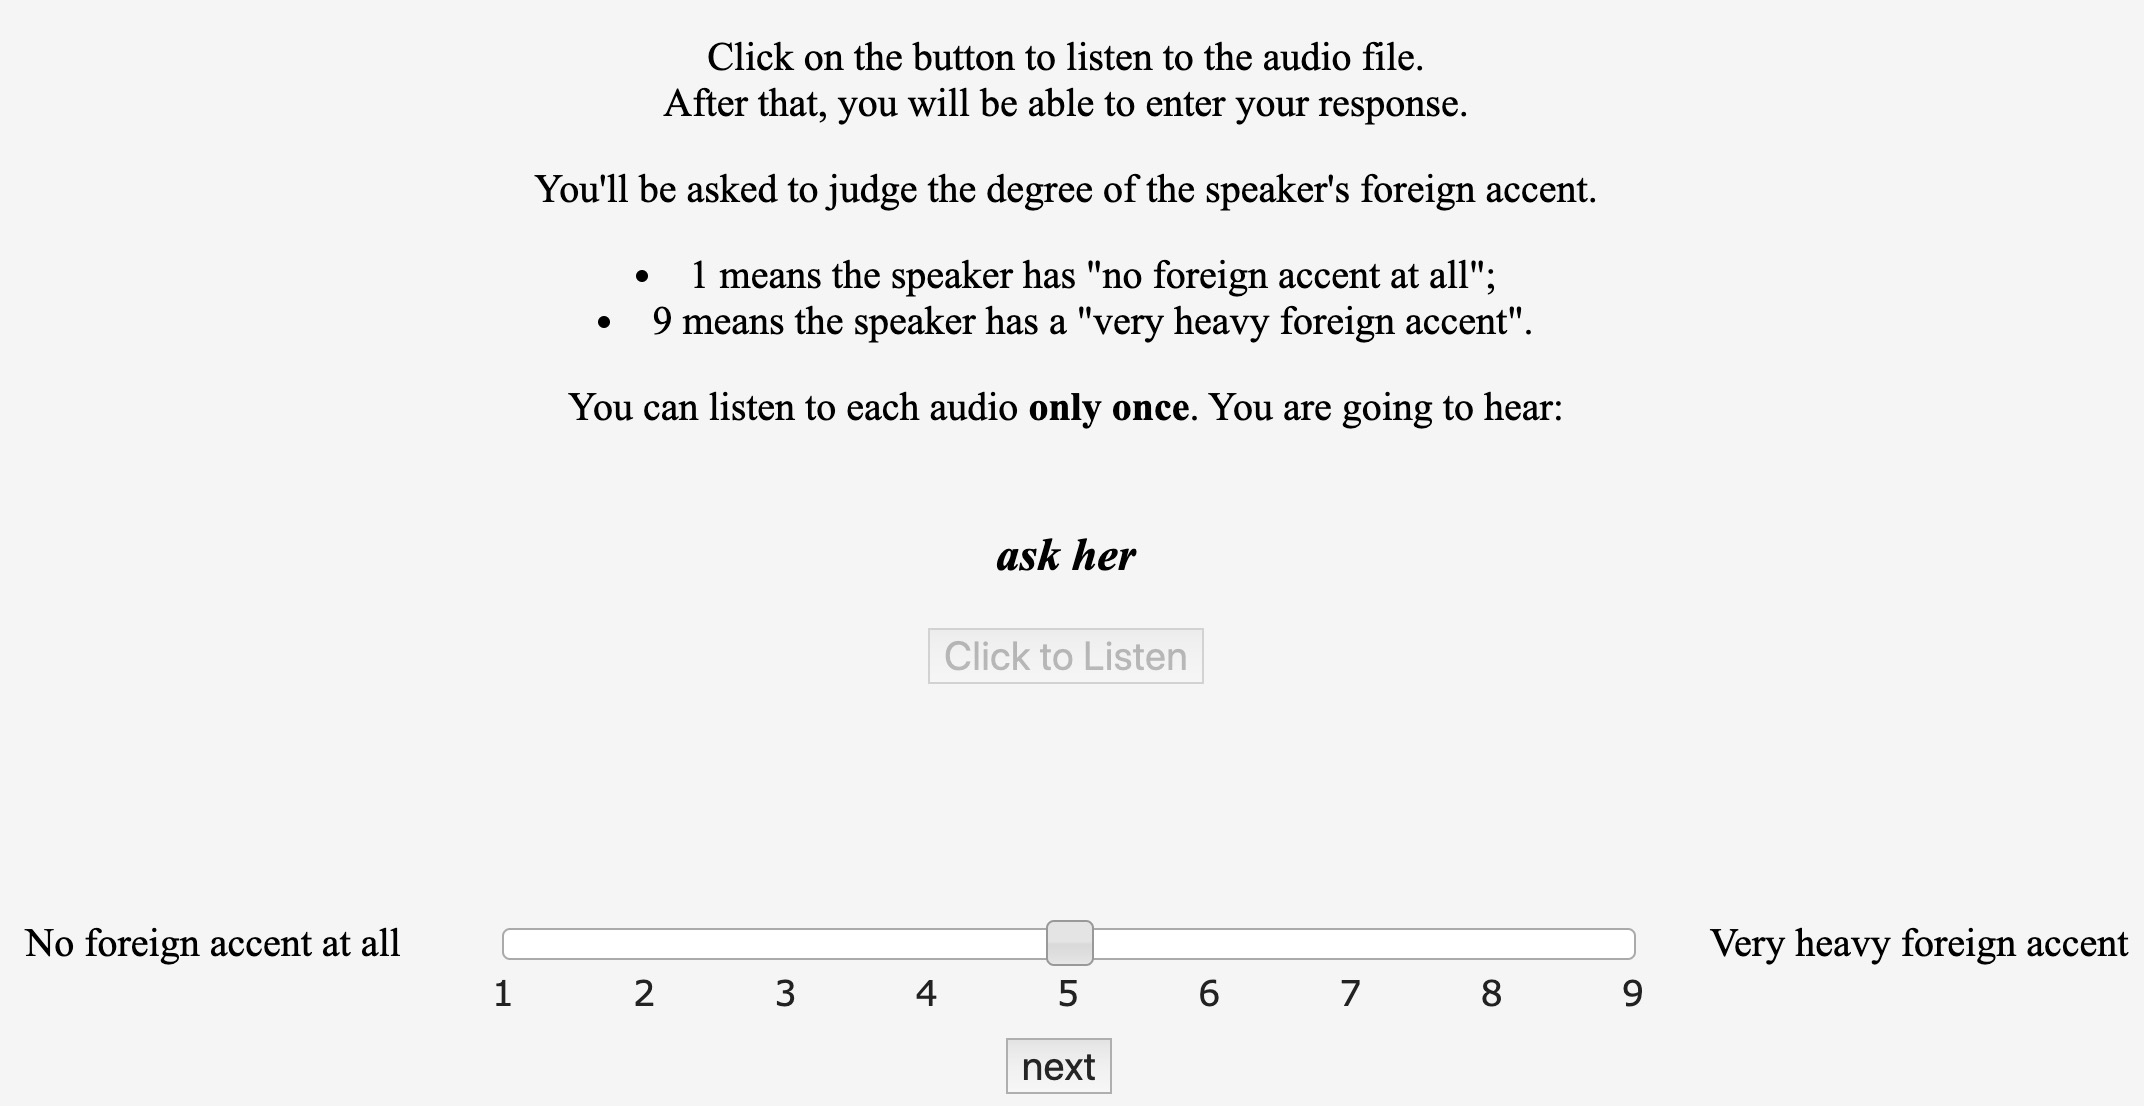
\includegraphics[width=0.8\linewidth]{figures/results/exp2/exp2.jpg}
\end{figure}
\end{frame}
%------------------------------------------------
\subsection{Raters}
\begin{frame}
\frametitle{Experiment 2: Rater Demographics}
\begin{itemize}
\item {133 participants (L1 American English speakers)}\linebreak
\item {Male:68, Female:58, 7 did not report}\linebreak
\item {Age: range 19-69 (M=38.42, SD=11.84)}\linebreak
\item {Completion Time: M=15.96 min, SD=5.47 min; \linebreak Maximum time allowed:40 min}
\end{itemize}
\end{frame}
%------------------------------------------------
\subsection{Results}
\begin{frame}
\frametitle{Experiment 2: Results}

\begin{block}{Meaning Ratings by Type}
%bar1 for Exp1
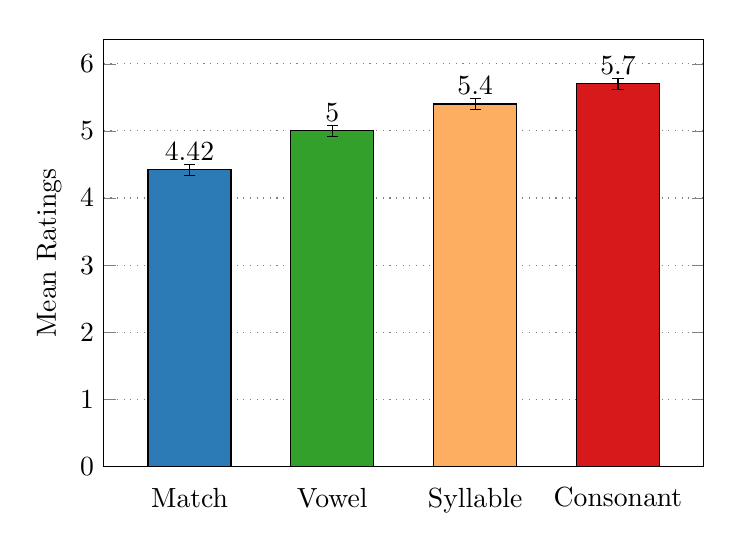
\begin{tikzpicture}
  \begin{axis}[
  ylabel={Mean Ratings},
width=9.2cm,
   height = 7cm,
    ytick distance=1,
        nodes near coords,
      major x tick style = transparent,
    ybar=3*\pgflinewidth,
      bar width=30pt,
      ymajorgrids = true,
      symbolic x coords={Match,Vowel,Syllable,Consonant},
      xtick ={Match,Vowel, Syllable, Consonant},
      scaled y ticks = false,
        legend style={at={(1.2,0.55)},
  anchor=north},
  legend cell align=left,
      enlarge x limits=0.20,
      ymin=0,
       every axis plot/.append style={
          ybar,
          bar shift=0pt,
          fill
        }
    ]
\addplot [fill=mycolor4,error bars/.cd, y dir=both, y explicit,error bar style=black] 
  coordinates {
          (Match, 4.42) += (0,0.08) -= (0,0.08)};
\addplot [fill=mycolor3,error bars/.cd, y dir=both, y explicit,error bar style=black] 
  coordinates {
          (Vowel, 5.00) += (0,0.08) -= (0,0.08)};
\addplot [fill=mycolor2,error bars/.cd, y dir=both, y explicit,error bar style=black] 
  coordinates {
          (Syllable, 5.40) += (0,0.08) -= (0,0.08)};
 \addplot [fill=mycolor1,error bars/.cd, y dir=both, y explicit,error bar style=black] 
  coordinates {
          (Consonant, 5.70) += (0,0.08) -= (0,0.08)};
 \end{axis}
\end{tikzpicture}



\end{block}

\end{frame}
%----------------
\begin{frame}[shrink=5]
\frametitle{Experiment 2:  Ratings across Time (SSANOVA)}
\begin{center}
% Created by tikzDevice version 0.12.3 on 2019-11-25 17:34:11
% !TEX encoding = UTF-8 Unicode
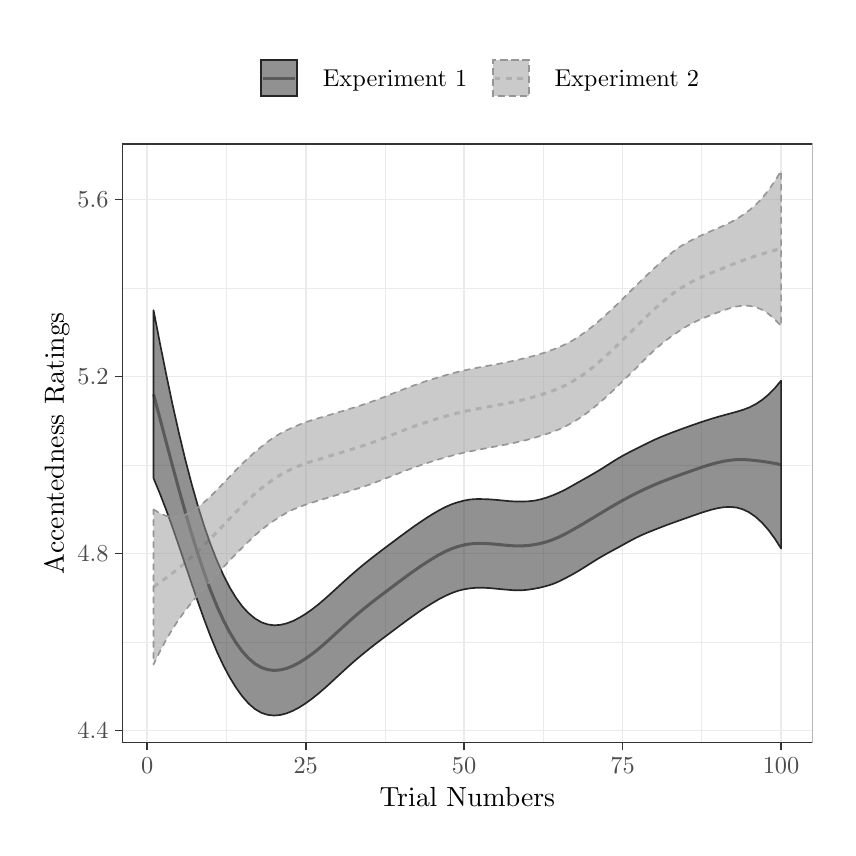
\begin{tikzpicture}[x=1pt,y=1pt]
\definecolor{fillColor}{RGB}{255,255,255}
\path[use as bounding box,fill=fillColor,fill opacity=0.00] (0,0) rectangle (289.08,289.08);
\begin{scope}
\path[clip] (  0.00,  0.00) rectangle (289.08,289.08);
\definecolor{drawColor}{RGB}{255,255,255}
\definecolor{fillColor}{RGB}{255,255,255}

\path[draw=drawColor,line width= 0.6pt,line join=round,line cap=round,fill=fillColor] (  0.00,  0.00) rectangle (289.08,289.08);
\end{scope}
\begin{scope}
\path[clip] ( 34.16, 30.69) rectangle (283.58,247.13);
\definecolor{fillColor}{RGB}{255,255,255}

\path[fill=fillColor] ( 34.16, 30.69) rectangle (283.58,247.13);
\definecolor{drawColor}{gray}{0.92}

\path[draw=drawColor,line width= 0.3pt,line join=round] ( 34.16, 67.10) --
	(283.58, 67.10);

\path[draw=drawColor,line width= 0.3pt,line join=round] ( 34.16,131.06) --
	(283.58,131.06);

\path[draw=drawColor,line width= 0.3pt,line join=round] ( 34.16,195.01) --
	(283.58,195.01);

\path[draw=drawColor,line width= 0.3pt,line join=round] ( 71.83, 30.69) --
	( 71.83,247.13);

\path[draw=drawColor,line width= 0.3pt,line join=round] (129.09, 30.69) --
	(129.09,247.13);

\path[draw=drawColor,line width= 0.3pt,line join=round] (186.35, 30.69) --
	(186.35,247.13);

\path[draw=drawColor,line width= 0.3pt,line join=round] (243.61, 30.69) --
	(243.61,247.13);

\path[draw=drawColor,line width= 0.6pt,line join=round] ( 34.16, 35.13) --
	(283.58, 35.13);

\path[draw=drawColor,line width= 0.6pt,line join=round] ( 34.16, 99.08) --
	(283.58, 99.08);

\path[draw=drawColor,line width= 0.6pt,line join=round] ( 34.16,163.03) --
	(283.58,163.03);

\path[draw=drawColor,line width= 0.6pt,line join=round] ( 34.16,226.99) --
	(283.58,226.99);

\path[draw=drawColor,line width= 0.6pt,line join=round] ( 43.20, 30.69) --
	( 43.20,247.13);

\path[draw=drawColor,line width= 0.6pt,line join=round] (100.46, 30.69) --
	(100.46,247.13);

\path[draw=drawColor,line width= 0.6pt,line join=round] (157.72, 30.69) --
	(157.72,247.13);

\path[draw=drawColor,line width= 0.6pt,line join=round] (214.98, 30.69) --
	(214.98,247.13);

\path[draw=drawColor,line width= 0.6pt,line join=round] (272.24, 30.69) --
	(272.24,247.13);
\definecolor{drawColor}{RGB}{37,37,37}

\path[draw=drawColor,draw opacity=0.50,line width= 1.1pt,line join=round] ( 45.49,156.60) --
	( 47.78,147.92) --
	( 50.07,139.25) --
	( 52.36,130.63) --
	( 54.66,122.19) --
	( 56.95,114.02) --
	( 59.24,106.21) --
	( 61.53, 98.84) --
	( 63.82, 91.98) --
	( 66.11, 85.68) --
	( 68.40, 80.02) --
	( 70.69, 75.00) --
	( 72.98, 70.61) --
	( 75.27, 66.84) --
	( 77.56, 63.69) --
	( 79.85, 61.16) --
	( 82.14, 59.22) --
	( 84.43, 57.88) --
	( 86.72, 57.10) --
	( 89.01, 56.83) --
	( 91.30, 57.00) --
	( 93.59, 57.57) --
	( 95.88, 58.47) --
	( 98.17, 59.67) --
	(100.46, 61.10) --
	(102.75, 62.75) --
	(105.04, 64.56) --
	(107.33, 66.51) --
	(109.62, 68.57) --
	(111.91, 70.69) --
	(114.21, 72.80) --
	(116.50, 74.86) --
	(118.79, 76.86) --
	(121.08, 78.78) --
	(123.37, 80.63) --
	(125.66, 82.42) --
	(127.95, 84.17) --
	(130.24, 85.88) --
	(132.53, 87.60) --
	(134.82, 89.32) --
	(137.11, 91.01) --
	(139.40, 92.66) --
	(141.69, 94.26) --
	(143.98, 95.78) --
	(146.27, 97.23) --
	(148.56, 98.57) --
	(150.85, 99.77) --
	(153.14,100.78) --
	(155.43,101.58) --
	(157.72,102.17) --
	(160.01,102.55) --
	(162.30,102.72) --
	(164.59,102.72) --
	(166.88,102.60) --
	(169.17,102.41) --
	(171.47,102.19) --
	(173.76,101.97) --
	(176.05,101.82) --
	(178.34,101.80) --
	(180.63,101.94) --
	(182.92,102.23) --
	(185.21,102.68) --
	(187.50,103.30) --
	(189.79,104.09) --
	(192.08,105.06) --
	(194.37,106.20) --
	(196.66,107.45) --
	(198.95,108.76) --
	(201.24,110.11) --
	(203.53,111.48) --
	(205.82,112.87) --
	(208.11,114.25) --
	(210.40,115.62) --
	(212.69,116.96) --
	(214.98,118.25) --
	(217.27,119.49) --
	(219.56,120.67) --
	(221.85,121.80) --
	(224.14,122.86) --
	(226.43,123.88) --
	(228.73,124.83) --
	(231.02,125.73) --
	(233.31,126.59) --
	(235.60,127.42) --
	(237.89,128.24) --
	(240.18,129.05) --
	(242.47,129.85) --
	(244.76,130.61) --
	(247.05,131.32) --
	(249.34,131.93) --
	(251.63,132.43) --
	(253.92,132.79) --
	(256.21,132.99) --
	(258.50,133.01) --
	(260.79,132.88) --
	(263.08,132.66) --
	(265.37,132.37) --
	(267.66,132.03) --
	(269.95,131.63) --
	(272.24,131.19);
\definecolor{drawColor}{RGB}{150,150,150}

\path[draw=drawColor,draw opacity=0.50,line width= 1.1pt,dash pattern=on 2pt off 2pt ,line join=round] ( 45.49, 87.00) --
	( 47.78, 88.64) --
	( 50.07, 90.32) --
	( 52.36, 92.03) --
	( 54.66, 93.84) --
	( 56.95, 95.76) --
	( 59.24, 97.78) --
	( 61.53, 99.92) --
	( 63.82,102.15) --
	( 66.11,104.47) --
	( 68.40,106.85) --
	( 70.69,109.26) --
	( 72.98,111.68) --
	( 75.27,114.06) --
	( 77.56,116.37) --
	( 79.85,118.58) --
	( 82.14,120.67) --
	( 84.43,122.62) --
	( 86.72,124.41) --
	( 89.01,126.03) --
	( 91.30,127.45) --
	( 93.59,128.71) --
	( 95.88,129.81) --
	( 98.17,130.77) --
	(100.46,131.62) --
	(102.75,132.38) --
	(105.04,133.07) --
	(107.33,133.75) --
	(109.62,134.43) --
	(111.91,135.12) --
	(114.21,135.82) --
	(116.50,136.53) --
	(118.79,137.25) --
	(121.08,137.99) --
	(123.37,138.77) --
	(125.66,139.60) --
	(127.95,140.47) --
	(130.24,141.37) --
	(132.53,142.28) --
	(134.82,143.19) --
	(137.11,144.07) --
	(139.40,144.92) --
	(141.69,145.72) --
	(143.98,146.49) --
	(146.27,147.23) --
	(148.56,147.94) --
	(150.85,148.61) --
	(153.14,149.24) --
	(155.43,149.83) --
	(157.72,150.37) --
	(160.01,150.86) --
	(162.30,151.31) --
	(164.59,151.74) --
	(166.88,152.17) --
	(169.17,152.59) --
	(171.47,153.02) --
	(173.76,153.48) --
	(176.05,153.95) --
	(178.34,154.47) --
	(180.63,155.04) --
	(182.92,155.67) --
	(185.21,156.34) --
	(187.50,157.08) --
	(189.79,157.90) --
	(192.08,158.81) --
	(194.37,159.87) --
	(196.66,161.10) --
	(198.95,162.50) --
	(201.24,164.07) --
	(203.53,165.81) --
	(205.82,167.69) --
	(208.11,169.69) --
	(210.40,171.78) --
	(212.69,173.94) --
	(214.98,176.16) --
	(217.27,178.42) --
	(219.56,180.70) --
	(221.85,182.96) --
	(224.14,185.18) --
	(226.43,187.34) --
	(228.73,189.39) --
	(231.02,191.33) --
	(233.31,193.11) --
	(235.60,194.72) --
	(237.89,196.13) --
	(240.18,197.37) --
	(242.47,198.48) --
	(244.76,199.50) --
	(247.05,200.46) --
	(249.34,201.39) --
	(251.63,202.31) --
	(253.92,203.23) --
	(256.21,204.15) --
	(258.50,205.02) --
	(260.79,205.84) --
	(263.08,206.59) --
	(265.37,207.31) --
	(267.66,207.98) --
	(269.95,208.64) --
	(272.24,209.28);
\definecolor{drawColor}{RGB}{37,37,37}
\definecolor{fillColor}{RGB}{37,37,37}

\path[draw=drawColor,line width= 0.6pt,line join=round,line cap=round,fill=fillColor,fill opacity=0.50] ( 45.49,186.96) --
	( 47.78,175.12) --
	( 50.07,163.72) --
	( 52.36,152.84) --
	( 54.66,142.58) --
	( 56.95,133.04) --
	( 59.24,124.23) --
	( 61.53,116.17) --
	( 63.82,108.85) --
	( 66.11,102.31) --
	( 68.40, 96.50) --
	( 70.69, 91.34) --
	( 72.98, 86.86) --
	( 75.27, 83.07) --
	( 77.56, 79.95) --
	( 79.85, 77.48) --
	( 82.14, 75.59) --
	( 84.43, 74.23) --
	( 86.72, 73.44) --
	( 89.01, 73.13) --
	( 91.30, 73.28) --
	( 93.59, 73.82) --
	( 95.88, 74.69) --
	( 98.17, 75.86) --
	(100.46, 77.27) --
	(102.75, 78.88) --
	(105.04, 80.67) --
	(107.33, 82.62) --
	(109.62, 84.67) --
	(111.91, 86.77) --
	(114.21, 88.88) --
	(116.50, 90.92) --
	(118.79, 92.92) --
	(121.08, 94.85) --
	(123.37, 96.69) --
	(125.66, 98.47) --
	(127.95,100.23) --
	(130.24,101.94) --
	(132.53,103.65) --
	(134.82,105.37) --
	(137.11,107.06) --
	(139.40,108.72) --
	(141.69,110.30) --
	(143.98,111.83) --
	(146.27,113.28) --
	(148.56,114.62) --
	(150.85,115.83) --
	(153.14,116.82) --
	(155.43,117.59) --
	(157.72,118.20) --
	(160.01,118.61) --
	(162.30,118.75) --
	(164.59,118.73) --
	(166.88,118.64) --
	(169.17,118.46) --
	(171.47,118.24) --
	(173.76,118.01) --
	(176.05,117.87) --
	(178.34,117.84) --
	(180.63,117.91) --
	(182.92,118.14) --
	(185.21,118.60) --
	(187.50,119.27) --
	(189.79,120.12) --
	(192.08,121.10) --
	(194.37,122.21) --
	(196.66,123.49) --
	(198.95,124.80) --
	(201.24,126.08) --
	(203.53,127.37) --
	(205.82,128.71) --
	(208.11,130.13) --
	(210.40,131.59) --
	(212.69,133.04) --
	(214.98,134.38) --
	(217.27,135.59) --
	(219.56,136.73) --
	(221.85,137.88) --
	(224.14,139.03) --
	(226.43,140.14) --
	(228.73,141.14) --
	(231.02,142.07) --
	(233.31,142.96) --
	(235.60,143.80) --
	(237.89,144.64) --
	(240.18,145.45) --
	(242.47,146.24) --
	(244.76,147.01) --
	(247.05,147.74) --
	(249.34,148.42) --
	(251.63,149.06) --
	(253.92,149.67) --
	(256.21,150.30) --
	(258.50,151.00) --
	(260.79,151.87) --
	(263.08,153.04) --
	(265.37,154.56) --
	(267.66,156.46) --
	(269.95,158.78) --
	(272.24,161.52) --
	(272.24,100.87) --
	(269.95,104.48) --
	(267.66,107.59) --
	(265.37,110.19) --
	(263.08,112.28) --
	(260.79,113.89) --
	(258.50,115.01) --
	(256.21,115.67) --
	(253.92,115.91) --
	(251.63,115.81) --
	(249.34,115.45) --
	(247.05,114.89) --
	(244.76,114.21) --
	(242.47,113.45) --
	(240.18,112.66) --
	(237.89,111.85) --
	(235.60,111.05) --
	(233.31,110.22) --
	(231.02,109.39) --
	(228.73,108.52) --
	(226.43,107.61) --
	(224.14,106.70) --
	(221.85,105.72) --
	(219.56,104.62) --
	(217.27,103.40) --
	(214.98,102.13) --
	(212.69,100.88) --
	(210.40, 99.65) --
	(208.11, 98.37) --
	(205.82, 97.02) --
	(203.53, 95.59) --
	(201.24, 94.13) --
	(198.95, 92.72) --
	(196.66, 91.41) --
	(194.37, 90.18) --
	(192.08, 89.02) --
	(189.79, 88.06) --
	(187.50, 87.33) --
	(185.21, 86.76) --
	(182.92, 86.31) --
	(180.63, 85.96) --
	(178.34, 85.77) --
	(176.05, 85.77) --
	(173.76, 85.94) --
	(171.47, 86.14) --
	(169.17, 86.36) --
	(166.88, 86.57) --
	(164.59, 86.71) --
	(162.30, 86.69) --
	(160.01, 86.50) --
	(157.72, 86.14) --
	(155.43, 85.57) --
	(153.14, 84.74) --
	(150.85, 83.72) --
	(148.56, 82.53) --
	(146.27, 81.17) --
	(143.98, 79.74) --
	(141.69, 78.22) --
	(139.40, 76.61) --
	(137.11, 74.96) --
	(134.82, 73.26) --
	(132.53, 71.54) --
	(130.24, 69.83) --
	(127.95, 68.11) --
	(125.66, 66.37) --
	(123.37, 64.57) --
	(121.08, 62.72) --
	(118.79, 60.81) --
	(116.50, 58.81) --
	(114.21, 56.72) --
	(111.91, 54.61) --
	(109.62, 52.48) --
	(107.33, 50.40) --
	(105.04, 48.44) --
	(102.75, 46.61) --
	(100.46, 44.94) --
	( 98.17, 43.47) --
	( 95.88, 42.26) --
	( 93.59, 41.32) --
	( 91.30, 40.72) --
	( 89.01, 40.52) --
	( 86.72, 40.77) --
	( 84.43, 41.52) --
	( 82.14, 42.85) --
	( 79.85, 44.83) --
	( 77.56, 47.43) --
	( 75.27, 50.62) --
	( 72.98, 54.35) --
	( 70.69, 58.65) --
	( 68.40, 63.55) --
	( 66.11, 69.06) --
	( 63.82, 75.10) --
	( 61.53, 81.51) --
	( 59.24, 88.20) --
	( 56.95, 95.00) --
	( 54.66,101.79) --
	( 52.36,108.42) --
	( 50.07,114.78) --
	( 47.78,120.71) --
	( 45.49,126.25) --
	cycle;
\definecolor{drawColor}{gray}{0.59}
\definecolor{fillColor}{RGB}{150,150,150}

\path[draw=drawColor,line width= 0.6pt,dash pattern=on 2pt off 2pt ,line join=round,line cap=round,fill=fillColor,fill opacity=0.50] ( 45.49,115.03) --
	( 47.78,113.59) --
	( 50.07,112.65) --
	( 52.36,112.24) --
	( 54.66,112.37) --
	( 56.95,113.04) --
	( 59.24,114.20) --
	( 61.53,115.76) --
	( 63.82,117.65) --
	( 66.11,119.76) --
	( 68.40,122.05) --
	( 70.69,124.44) --
	( 72.98,126.82) --
	( 75.27,129.20) --
	( 77.56,131.53) --
	( 79.85,133.70) --
	( 82.14,135.72) --
	( 84.43,137.64) --
	( 86.72,139.45) --
	( 89.01,141.09) --
	( 91.30,142.45) --
	( 93.59,143.61) --
	( 95.88,144.66) --
	( 98.17,145.64) --
	(100.46,146.53) --
	(102.75,147.28) --
	(105.04,147.96) --
	(107.33,148.62) --
	(109.62,149.29) --
	(111.91,149.99) --
	(114.21,150.67) --
	(116.50,151.39) --
	(118.79,152.08) --
	(121.08,152.82) --
	(123.37,153.62) --
	(125.66,154.42) --
	(127.95,155.27) --
	(130.24,156.20) --
	(132.53,157.13) --
	(134.82,158.03) --
	(137.11,158.93) --
	(139.40,159.76) --
	(141.69,160.57) --
	(143.98,161.35) --
	(146.27,162.07) --
	(148.56,162.78) --
	(150.85,163.46) --
	(153.14,164.09) --
	(155.43,164.68) --
	(157.72,165.22) --
	(160.01,165.71) --
	(162.30,166.15) --
	(164.59,166.59) --
	(166.88,167.00) --
	(169.17,167.40) --
	(171.47,167.86) --
	(173.76,168.33) --
	(176.05,168.80) --
	(178.34,169.32) --
	(180.63,169.90) --
	(182.92,170.50) --
	(185.21,171.16) --
	(187.50,171.92) --
	(189.79,172.75) --
	(192.08,173.66) --
	(194.37,174.71) --
	(196.66,175.91) --
	(198.95,177.33) --
	(201.24,178.92) --
	(203.53,180.65) --
	(205.82,182.54) --
	(208.11,184.55) --
	(210.40,186.65) --
	(212.69,188.80) --
	(214.98,191.02) --
	(217.27,193.33) --
	(219.56,195.62) --
	(221.85,197.83) --
	(224.14,200.00) --
	(226.43,202.14) --
	(228.73,204.26) --
	(231.02,206.30) --
	(233.31,208.20) --
	(235.60,209.85) --
	(237.89,211.22) --
	(240.18,212.42) --
	(242.47,213.56) --
	(244.76,214.63) --
	(247.05,215.63) --
	(249.34,216.60) --
	(251.63,217.61) --
	(253.92,218.71) --
	(256.21,219.96) --
	(258.50,221.43) --
	(260.79,223.11) --
	(263.08,225.07) --
	(265.37,227.44) --
	(267.66,230.28) --
	(269.95,233.58) --
	(272.24,237.29) --
	(272.24,181.28) --
	(269.95,183.70) --
	(267.66,185.69) --
	(265.37,187.17) --
	(263.08,188.11) --
	(260.79,188.56) --
	(258.50,188.62) --
	(256.21,188.34) --
	(253.92,187.76) --
	(251.63,187.01) --
	(249.34,186.18) --
	(247.05,185.29) --
	(244.76,184.36) --
	(242.47,183.40) --
	(240.18,182.32) --
	(237.89,181.04) --
	(235.60,179.59) --
	(233.31,178.03) --
	(231.02,176.36) --
	(228.73,174.53) --
	(226.43,172.53) --
	(224.14,170.36) --
	(221.85,168.08) --
	(219.56,165.77) --
	(217.27,163.51) --
	(214.98,161.30) --
	(212.69,159.08) --
	(210.40,156.90) --
	(208.11,154.82) --
	(205.82,152.85) --
	(203.53,150.97) --
	(201.24,149.22) --
	(198.95,147.67) --
	(196.66,146.29) --
	(194.37,145.04) --
	(192.08,143.96) --
	(189.79,143.05) --
	(187.50,142.25) --
	(185.21,141.53) --
	(182.92,140.83) --
	(180.63,140.19) --
	(178.34,139.63) --
	(176.05,139.10) --
	(173.76,138.62) --
	(171.47,138.19) --
	(169.17,137.78) --
	(166.88,137.33) --
	(164.59,136.89) --
	(162.30,136.47) --
	(160.01,136.01) --
	(157.72,135.52) --
	(155.43,134.99) --
	(153.14,134.39) --
	(150.85,133.76) --
	(148.56,133.10) --
	(146.27,132.39) --
	(143.98,131.64) --
	(141.69,130.87) --
	(139.40,130.07) --
	(137.11,129.22) --
	(134.82,128.35) --
	(132.53,127.43) --
	(130.24,126.54) --
	(127.95,125.66) --
	(125.66,124.77) --
	(123.37,123.92) --
	(121.08,123.16) --
	(118.79,122.41) --
	(116.50,121.67) --
	(114.21,120.97) --
	(111.91,120.26) --
	(109.62,119.58) --
	(107.33,118.88) --
	(105.04,118.18) --
	(102.75,117.47) --
	(100.46,116.71) --
	( 98.17,115.90) --
	( 95.88,114.95) --
	( 93.59,113.81) --
	( 91.30,112.46) --
	( 89.01,110.97) --
	( 86.72,109.36) --
	( 84.43,107.59) --
	( 82.14,105.61) --
	( 79.85,103.45) --
	( 77.56,101.20) --
	( 75.27, 98.92) --
	( 72.98, 96.53) --
	( 70.69, 94.08) --
	( 68.40, 91.65) --
	( 66.11, 89.17) --
	( 63.82, 86.64) --
	( 61.53, 84.07) --
	( 59.24, 81.36) --
	( 56.95, 78.47) --
	( 54.66, 75.31) --
	( 52.36, 71.83) --
	( 50.07, 67.98) --
	( 47.78, 63.70) --
	( 45.49, 58.97) --
	cycle;
\definecolor{drawColor}{gray}{0.20}

\path[draw=drawColor,line width= 0.6pt,line join=round,line cap=round] ( 34.16, 30.69) rectangle (283.58,247.13);
\end{scope}
\begin{scope}
\path[clip] (  0.00,  0.00) rectangle (289.08,289.08);
\definecolor{drawColor}{gray}{0.30}

\node[text=drawColor,anchor=base east,inner sep=0pt, outer sep=0pt, scale=  0.88] at ( 29.21, 32.10) {4.4};

\node[text=drawColor,anchor=base east,inner sep=0pt, outer sep=0pt, scale=  0.88] at ( 29.21, 96.05) {4.8};

\node[text=drawColor,anchor=base east,inner sep=0pt, outer sep=0pt, scale=  0.88] at ( 29.21,160.00) {5.2};

\node[text=drawColor,anchor=base east,inner sep=0pt, outer sep=0pt, scale=  0.88] at ( 29.21,223.96) {5.6};
\end{scope}
\begin{scope}
\path[clip] (  0.00,  0.00) rectangle (289.08,289.08);
\definecolor{drawColor}{gray}{0.20}

\path[draw=drawColor,line width= 0.6pt,line join=round] ( 31.41, 35.13) --
	( 34.16, 35.13);

\path[draw=drawColor,line width= 0.6pt,line join=round] ( 31.41, 99.08) --
	( 34.16, 99.08);

\path[draw=drawColor,line width= 0.6pt,line join=round] ( 31.41,163.03) --
	( 34.16,163.03);

\path[draw=drawColor,line width= 0.6pt,line join=round] ( 31.41,226.99) --
	( 34.16,226.99);
\end{scope}
\begin{scope}
\path[clip] (  0.00,  0.00) rectangle (289.08,289.08);
\definecolor{drawColor}{gray}{0.20}

\path[draw=drawColor,line width= 0.6pt,line join=round] ( 43.20, 27.94) --
	( 43.20, 30.69);

\path[draw=drawColor,line width= 0.6pt,line join=round] (100.46, 27.94) --
	(100.46, 30.69);

\path[draw=drawColor,line width= 0.6pt,line join=round] (157.72, 27.94) --
	(157.72, 30.69);

\path[draw=drawColor,line width= 0.6pt,line join=round] (214.98, 27.94) --
	(214.98, 30.69);

\path[draw=drawColor,line width= 0.6pt,line join=round] (272.24, 27.94) --
	(272.24, 30.69);
\end{scope}
\begin{scope}
\path[clip] (  0.00,  0.00) rectangle (289.08,289.08);
\definecolor{drawColor}{gray}{0.30}

\node[text=drawColor,anchor=base,inner sep=0pt, outer sep=0pt, scale=  0.88] at ( 43.20, 19.68) {0};

\node[text=drawColor,anchor=base,inner sep=0pt, outer sep=0pt, scale=  0.88] at (100.46, 19.68) {25};

\node[text=drawColor,anchor=base,inner sep=0pt, outer sep=0pt, scale=  0.88] at (157.72, 19.68) {50};

\node[text=drawColor,anchor=base,inner sep=0pt, outer sep=0pt, scale=  0.88] at (214.98, 19.68) {75};

\node[text=drawColor,anchor=base,inner sep=0pt, outer sep=0pt, scale=  0.88] at (272.24, 19.68) {100};
\end{scope}
\begin{scope}
\path[clip] (  0.00,  0.00) rectangle (289.08,289.08);
\definecolor{drawColor}{RGB}{0,0,0}

\node[text=drawColor,anchor=base,inner sep=0pt, outer sep=0pt, scale=  1.00] at (158.87,  7.64) {Trial Numbers};
\end{scope}
\begin{scope}
\path[clip] (  0.00,  0.00) rectangle (289.08,289.08);
\definecolor{drawColor}{RGB}{0,0,0}

\node[text=drawColor,rotate= 90.00,anchor=base,inner sep=0pt, outer sep=0pt, scale=  1.00] at ( 13.08,138.91) {Accentedness Ratings};
\end{scope}
\begin{scope}
\path[clip] (  0.00,  0.00) rectangle (289.08,289.08);
\definecolor{fillColor}{RGB}{255,255,255}

\path[fill=fillColor] ( 69.64,258.13) rectangle (248.09,283.58);
\end{scope}
\begin{scope}
\path[clip] (  0.00,  0.00) rectangle (289.08,289.08);
\definecolor{fillColor}{RGB}{255,255,255}

\path[fill=fillColor] ( 83.68,263.63) rectangle ( 98.13,278.08);
\end{scope}
\begin{scope}
\path[clip] (  0.00,  0.00) rectangle (289.08,289.08);
\definecolor{drawColor}{RGB}{37,37,37}

\path[draw=drawColor,draw opacity=0.50,line width= 1.1pt,line join=round] ( 85.12,270.85) -- ( 96.69,270.85);
\end{scope}
\begin{scope}
\path[clip] (  0.00,  0.00) rectangle (289.08,289.08);
\definecolor{drawColor}{RGB}{37,37,37}
\definecolor{fillColor}{RGB}{37,37,37}

\path[draw=drawColor,line width= 0.6pt,line cap=rect,fill=fillColor,fill opacity=0.50] ( 84.39,264.34) rectangle ( 97.42,277.37);
\end{scope}
\begin{scope}
\path[clip] (  0.00,  0.00) rectangle (289.08,289.08);
\definecolor{fillColor}{RGB}{255,255,255}

\path[fill=fillColor] (167.40,263.63) rectangle (181.86,278.08);
\end{scope}
\begin{scope}
\path[clip] (  0.00,  0.00) rectangle (289.08,289.08);
\definecolor{drawColor}{RGB}{150,150,150}

\path[draw=drawColor,draw opacity=0.50,line width= 1.1pt,dash pattern=on 2pt off 2pt ,line join=round] (168.85,270.85) -- (180.41,270.85);
\end{scope}
\begin{scope}
\path[clip] (  0.00,  0.00) rectangle (289.08,289.08);
\definecolor{drawColor}{gray}{0.59}
\definecolor{fillColor}{RGB}{150,150,150}

\path[draw=drawColor,line width= 0.6pt,dash pattern=on 2pt off 2pt ,line cap=rect,fill=fillColor,fill opacity=0.50] (168.12,264.34) rectangle (181.15,277.37);
\end{scope}
\begin{scope}
\path[clip] (  0.00,  0.00) rectangle (289.08,289.08);
\definecolor{drawColor}{RGB}{0,0,0}

\node[text=drawColor,anchor=base west,inner sep=0pt, outer sep=0pt, scale=  0.88] at (106.67,267.82) {Experiment 1};
\end{scope}
\begin{scope}
\path[clip] (  0.00,  0.00) rectangle (289.08,289.08);
\definecolor{drawColor}{RGB}{0,0,0}

\node[text=drawColor,anchor=base west,inner sep=0pt, outer sep=0pt, scale=  0.88] at (190.39,267.82) {Experiment 2};
\end{scope}
\end{tikzpicture}

\end{center}
\end{frame}
%------------------
\begin{frame}
\frametitle{Experiment 2:  L1 Dialectal vs. Non-dialectal}
\begin{center}
\begin{spacing}{2}
{\color{red} θ$\rightarrow$s̪t̪ } is more accented than \textbf{θ$\rightarrow$t̪} and \textbf{θ$\rightarrow$f} 
\end{spacing}
\begin{block}{/θ/ changes in ``five thick"}
\centering

\begin{tikzpicture}
  \begin{axis}[
  title={Mean Accentedness Ratings},
     % xbar,
   ytick={1,2,3,4,5,6,7,8,9},
     y=1cm,
  bar width=0.7 cm,
  xmin=0,
  xmax=7.5,
    axis y line*=left,
   axis x line=bottom,
    tickwidth         = 1pt,
    enlarge y limits  = 0.1,
    enlarge x limits  = 0.02,
  legend style={at={(1.2,0.55)},
  anchor=north},
  legend cell align=left,
      yticklabels from table={figures/bar2/data_fth.txt}{label},
      xtick distance=2,
      every axis plot/.append style={
          xbar,
          bar shift=0pt,
          fill
        }
    ]
\addplot [fill=red,color=mycolor3,select coords between index={0}{0}] table  [x=x,y=y] {figures/bar2/data_fth.txt};
\addplot [fill=red,color=mycolor1,select coords between index={1}{1}] table  [x=x,y=y] {figures/bar2/data_fth.txt};
\addplot [fill=blue,color=mycolor3,select coords between index={2}{9}] table [x=x, y=y] {figures/bar2/data_fth.txt};
 \addplot [color=black, only marks, mark=o]
 plot [error bars/.cd, x dir = both, x explicit]
 table[x =x, y =y, x error =err]{figures/bar2/data_fth.txt};
 \end{axis}
 \node[] at (6.91,8.7) {6.35};
\node[] at (6.75,7.7) {6.11};
\node[] at (6.67,6.7) {6.03};
\node[] at (5.93,5.7) {5.42};
\node[] at (6.01,4.7) {5.36};
\node[] at (5.65,3.7) {4.14};
\node[] at (5.62,2.7) {4.92};
\node[] at (4.92,1.7) {4.43};
\node[] at (4.91,0.7) {4.40};


\end{tikzpicture}

\end{block}
\end{center}
\end{frame}
%-----------------
\begin{frame}[shrink=10]
\frametitle{Experiment 2:  Phonological Environment}
\begin{spacing}{2}
\centering
\only<1>{
/k/-deletion in ``ask her" vs. other coda deletions \linebreak
\begin{block}{Coda Deletions }
\centering
%consonant0deletion
\begin{tikzpicture}
  \begin{axis}[
  title={Mean Accentedness Ratings},
     % xbar,
   ytick={1,2,3,4},
     y=-1.2cm,
  bar width=0.8cm,
  xmin=0,
  xmax=6,
     %y axis line style = { opacity = 0 },
     axis y line*=left,
   axis x line=bottom,
    tickwidth         = 1pt,
    enlarge y limits  = 0.2,
    enlarge x limits  = 0.02,
  legend style={at={(1.2,0.55)},
  anchor=north},
  legend cell align=left,
      yticklabels from table={figures/bar1/cdel.txt}{label},
      xtick distance=2,
      every axis plot/.append style={
          xbar,
          bar shift=0pt,
          fill
        }
    ]
\addplot [fill=red,color=mycolor1,select coords between index={0}{0}] table  [x=x,y=y] {figures/bar1/cdel.txt};
\addplot [fill=blue,color=mycolor3,select coords between index={1}{3}] table [x=x, y=y] {figures/bar1/cdel.txt};
 \addplot [color=black, only marks, mark=o]
 plot [error bars/.cd, x dir = both, x explicit]
 table[x =x, y =y, x error =err]{figures/bar1/cdel.txt};
 \end{axis}
 \node[] at (7.2,2.8){*};
\end{tikzpicture}
\end{block}
}
\only<2>{
Phrase-Initial vs. Phrase-Medial VOT-shortening \linebreak
\begin{block}{VOT-shortenings}
\centering
\begin{tikzpicture}
  \begin{axis}[
  title={Mean Accentedness Ratings},
     % xbar,
   ytick={1,2,3},
     y=-1.5cm,
  bar width=1cm,
  xmin=0,
  xmax=7.5,
    axis y line*=left,
   axis x line=bottom,
    tickwidth         = 1pt,
    enlarge y limits  = 0.2,
    enlarge x limits  = 0.02,
  legend style={at={(1.2,0.55)},
  anchor=north},
  legend cell align=left,
      yticklabels from table={figures/results/exp2/data.txt}{label},
      xtick distance=2,
      every axis plot/.append style={
          xbar,
          bar shift=0pt,
          fill
        }
    ]
\addplot [fill=red,color=mycolor1,select coords between index={0}{0}] table  [x=x,y=y] {figures/results/exp2/data.txt};
\addplot [fill=blue,color=mycolor4,select coords between index={1}{2}] table [x=x, y=y] {figures/results/exp2/data.txt};
 \addplot [color=black, only marks, mark=o]
 plot [error bars/.cd, x dir = both, x explicit]
 table[x =x, y =y, x error =err]{figures/results/exp2/data.txt};
 \legend{Phrase-initial,Phrase-medial}
 \end{axis}
\node[] at (6.8,3.5) {*};
\end{tikzpicture}
\end{block}
}
\end{spacing}
\end{frame}
%------------------
\subsection{Summary}
\begin{frame}
\frametitle{Experiment 2: Summary}
\centering
\textbf{What affects accentedness judgment?}\linebreak
\begin{itemize}
\onslide<1->{\item[1] \textbf{Lexical Information}\linebreak Ratings became higher when the intended meanings were known. }\linebreak
\onslide<2->{\item[2] \textbf{Frequency of occurrences of a ``mismatch" in L1 speech} \linebreak e.g., ``thick" /stɪk/ vs. /tɪk/ vs. /fɪk/ vs. /θɪk/} \linebreak
\onslide<3->{\item[3] \textbf{Phonological environment} \linebreak e.g., /k/-deletion in ``ask her", \linebreak Phrase-initial vs. phrase-medial VOT-shortening}
\end{itemize}
\end{frame}
%------------------
\section{Experiment 3}
\subsection{Introduction}
\begin{frame}
\frametitle{Experiment 3: Introduction}
\textbf{Hypothesis: }
\begin{itemize}
	\item[] (1) Lexical information
	\item[] (2) Occurrences in L1 speech
		$\smash{\left.\rule{0pt}{.5\dimexpr3\baselineskip+3\itemsep+2\parskip}\right\}
     		\text{\parbox{6cm}{L1 Knowledge --> Accent judgment}}}$
	\item[] (3) Phonological environment
\end{itemize}
\textbf{Aim:} \linebreak
Build a computational model to verify that L1 knowledge affects accentedness judgment.
\end{frame}
%------------------
\subsection{Method}
\begin{frame}
\frametitle{Experiment 3: Method}

\only<1>{
The Naïve Discriminative Learning Model (\textbf{NDL Model})\linebreak
\textsubscript{(Wieling et al. 2014; Bayaan, 2011)}\linebreak\linebreak
Rescorla-Wagner learning theory (1972): learners attempt to predict an outcome based on available cues. \linebreak
\linebreak \textbf{Cue:} Four-legged \linebreak
\textbf{Outcomes:} Puppy, Kitten, Table, Chair etc. \linebreak
\textbf{Association Strength (Weight)}: \linebreak How probably the cue ``Four-legged" can predict outcome ``Puppy". 
}

\only<2>{
Data: Productions from 100 L1 American English Speakers \linebreak
Cues: Trigram sequences \linebreak
Outcomes: Words \linebreak

\begin{table}[!h]
  \centering
  \caption{Association Strengths}
    \begin{tabular}{llr}
    \toprule
    Cues & Outcomes  & Association Strengths \\
    \midrule
     \#æs  & ask & 0.166 \\
      æsk  & ask &0.167 \\
     sk\#  & ask &0.667 \\
     \#æ̞s & ask &0.147\\
     æ̞sk & ask &0.147\\
     \#ɚ\#  & her & 1.000 \\
     \#hɚ  & her &0.500 \\
     hɚ\#  & her & 0.500 \\
    \bottomrule
    \end{tabular}%
  \label{tab:strength}%
\end{table}%
}

\only<3>{
Reasons for using Trigram cues:
\begin{itemize}
\item [1] \textbf{Three-member sequence}: English phonotactics, sound changes in continuous speech
\item [2] \textbf{Include diacritics}: Sub-phonemic information ( {[æ]} and {[æ̞]} are two independent segments)
\item [3] \textbf{Lexical outcomes}: Lexical information
\end{itemize}
}
\end{frame}
%------------------
\begin{frame}[shrink=10]
\frametitle{Experiment 3: Method}

\begin{table}[]
\begin{tabular}{lcl}
\toprule
 Pronunciation & Association Strength  & NDL-distance \\
 \midrule
 {[æsk.ɚ]} & $(0.166+0.167+0.667+1.000)\div 2 = 1.000$ & $1-1.000=0.000$  \\
  {[æ̞sk.ɚ]} & $(0.147+0.147+0.667+1.000)\div 2 = 0.980$ & $1-0.980=0.020$  \\
 {[ask.hɚ]} & $(0+0+0.667+0.500+0.500)\div 2 = 0.834$ & $1-0.834=0.166 $  \\
 \bottomrule
\end{tabular}
\end{table}
\begin{table}[!h]
  \centering
  \caption{Association Strengths}
    \begin{tabular}{ccc}
    \toprule
    Cues & Outcomes  & Association Strengths \\
    \midrule
 \#æs  & ask & 0.166 \\
      æsk  & ask &0.167 \\
     sk\#  & ask &0.667 \\
     \#æ̞s & ask &0.147\\
     æ̞sk & ask &0.147\\
     \#ɚ\#  & her & 1.000 \\
     \#hɚ  & her &0.500 \\
     hɚ\#  & her & 0.500 \\
    \bottomrule
    \end{tabular}%
  \label{tab:strength}%
\end{table}%



\end{frame}
%------------------
%------------------
\begin{frame}
\frametitle{Experiment 3: The NDL model}
Try out the NDL model at \url{https://gaozhiyan.shinyapps.io/ndl_calculator/}
\begin{block}{A Web Application}
\begin{figure}
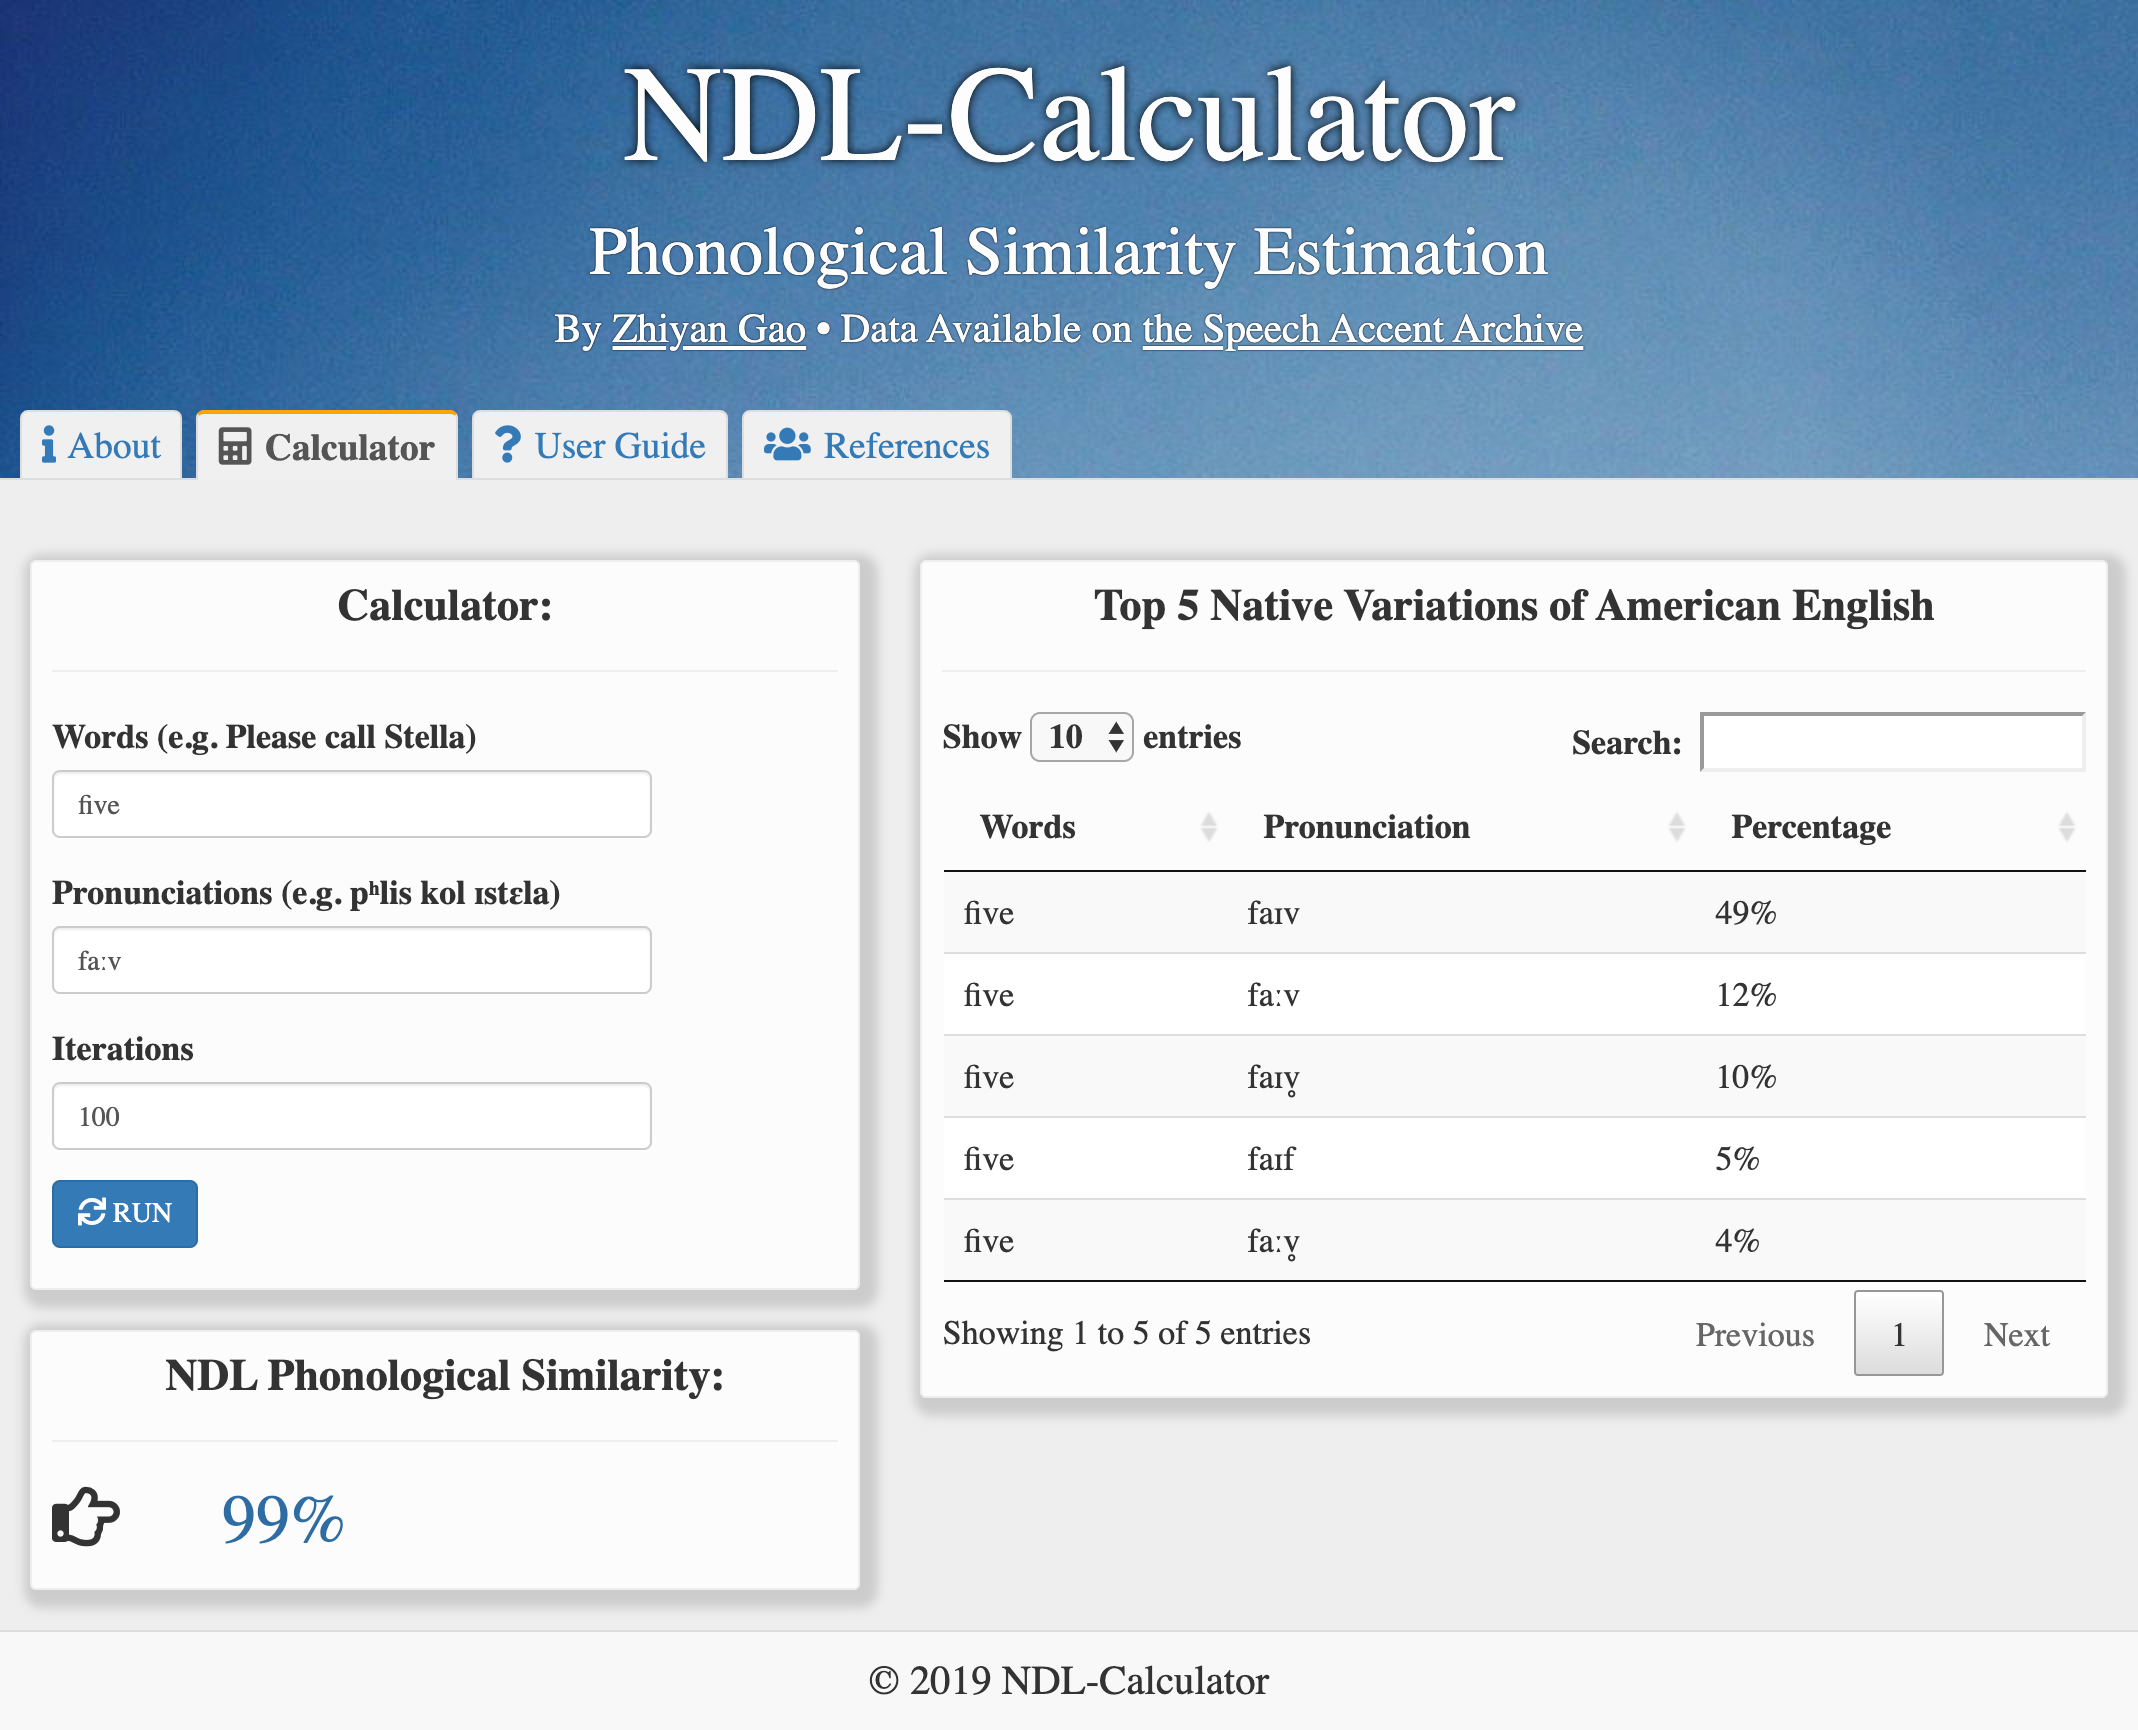
\includegraphics[width=0.7\linewidth]{figures/ndl.png}
\end{figure}
\end{block}
\end{frame}
%--------------------
\begin{frame}[shrink=10]
\frametitle{Experiment 3: Results}
\begin{center}
% Created by tikzDevice version 0.12.3 on 2019-11-25 14:05:33
% !TEX encoding = UTF-8 Unicode
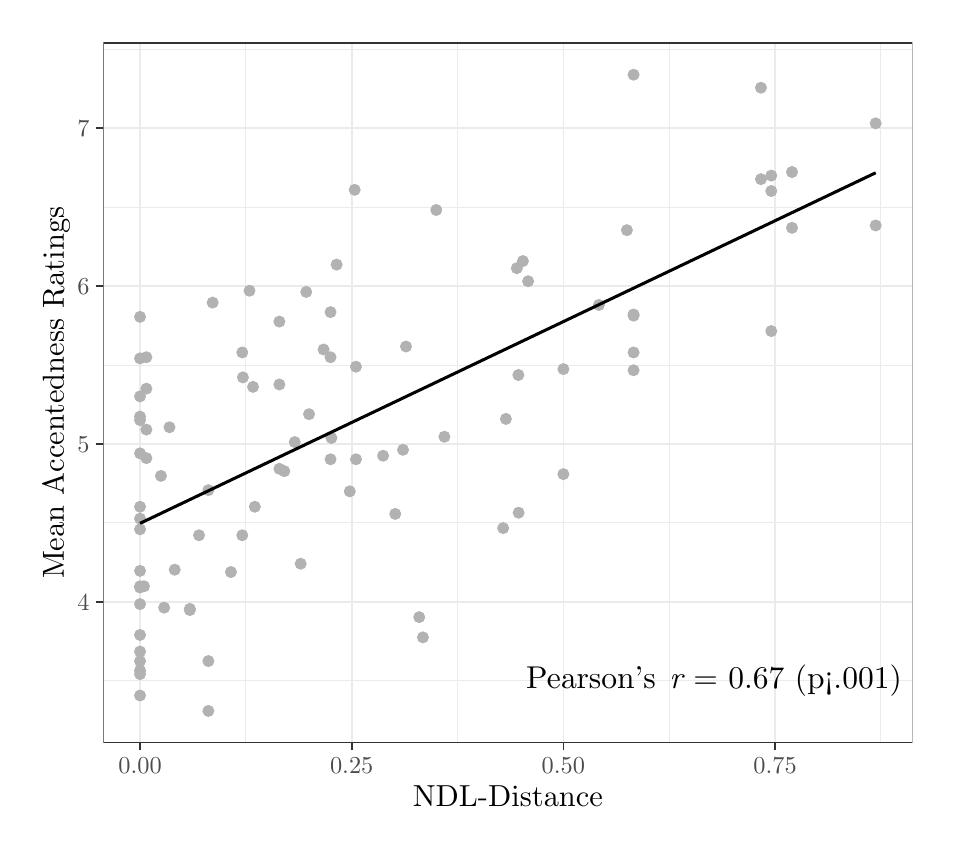
\begin{tikzpicture}[x=1pt,y=1pt]
\definecolor{fillColor}{RGB}{255,255,255}
\path[use as bounding box,fill=fillColor,fill opacity=0.00] (0,0) rectangle (325.21,289.08);
\begin{scope}
\path[clip] (  0.00,  0.00) rectangle (325.21,289.08);
\definecolor{drawColor}{RGB}{255,255,255}
\definecolor{fillColor}{RGB}{255,255,255}

\path[draw=drawColor,line width= 0.6pt,line join=round,line cap=round,fill=fillColor] (  0.00,  0.00) rectangle (325.21,289.08);
\end{scope}
\begin{scope}
\path[clip] ( 27.31, 30.69) rectangle (319.71,283.58);
\definecolor{fillColor}{RGB}{255,255,255}

\path[fill=fillColor] ( 27.31, 30.69) rectangle (319.71,283.58);
\definecolor{drawColor}{gray}{0.92}

\path[draw=drawColor,line width= 0.3pt,line join=round] ( 27.31, 53.12) --
	(319.71, 53.12);

\path[draw=drawColor,line width= 0.3pt,line join=round] ( 27.31,110.17) --
	(319.71,110.17);

\path[draw=drawColor,line width= 0.3pt,line join=round] ( 27.31,167.21) --
	(319.71,167.21);

\path[draw=drawColor,line width= 0.3pt,line join=round] ( 27.31,224.26) --
	(319.71,224.26);

\path[draw=drawColor,line width= 0.3pt,line join=round] ( 27.31,281.31) --
	(319.71,281.31);

\path[draw=drawColor,line width= 0.3pt,line join=round] ( 78.85, 30.69) --
	( 78.85,283.58);

\path[draw=drawColor,line width= 0.3pt,line join=round] (155.34, 30.69) --
	(155.34,283.58);

\path[draw=drawColor,line width= 0.3pt,line join=round] (231.82, 30.69) --
	(231.82,283.58);

\path[draw=drawColor,line width= 0.3pt,line join=round] (308.31, 30.69) --
	(308.31,283.58);

\path[draw=drawColor,line width= 0.6pt,line join=round] ( 27.31, 81.64) --
	(319.71, 81.64);

\path[draw=drawColor,line width= 0.6pt,line join=round] ( 27.31,138.69) --
	(319.71,138.69);

\path[draw=drawColor,line width= 0.6pt,line join=round] ( 27.31,195.74) --
	(319.71,195.74);

\path[draw=drawColor,line width= 0.6pt,line join=round] ( 27.31,252.78) --
	(319.71,252.78);

\path[draw=drawColor,line width= 0.6pt,line join=round] ( 40.60, 30.69) --
	( 40.60,283.58);

\path[draw=drawColor,line width= 0.6pt,line join=round] (117.09, 30.69) --
	(117.09,283.58);

\path[draw=drawColor,line width= 0.6pt,line join=round] (193.58, 30.69) --
	(193.58,283.58);

\path[draw=drawColor,line width= 0.6pt,line join=round] (270.07, 30.69) --
	(270.07,283.58);
\definecolor{drawColor}{gray}{0.70}
\definecolor{fillColor}{gray}{0.70}

\path[draw=drawColor,line width= 0.4pt,line join=round,line cap=round,fill=fillColor] ( 96.50,139.33) circle (  1.96);

\path[draw=drawColor,line width= 0.4pt,line join=round,line cap=round,fill=fillColor] (306.42,217.61) circle (  1.96);

\path[draw=drawColor,line width= 0.4pt,line join=round,line cap=round,fill=fillColor] (118.62,133.11) circle (  1.96);

\path[draw=drawColor,line width= 0.4pt,line join=round,line cap=round,fill=fillColor] ( 61.91,105.66) circle (  1.96);

\path[draw=drawColor,line width= 0.4pt,line join=round,line cap=round,fill=fillColor] (218.94,185.44) circle (  1.96);

\path[draw=drawColor,line width= 0.4pt,line join=round,line cap=round,fill=fillColor] ( 40.60, 60.20) circle (  1.96);

\path[draw=drawColor,line width= 0.4pt,line join=round,line cap=round,fill=fillColor] (136.70,173.86) circle (  1.96);

\path[draw=drawColor,line width= 0.4pt,line join=round,line cap=round,fill=fillColor] (218.94,171.72) circle (  1.96);

\path[draw=drawColor,line width= 0.4pt,line join=round,line cap=round,fill=fillColor] ( 58.60, 79.07) circle (  1.96);

\path[draw=drawColor,line width= 0.4pt,line join=round,line cap=round,fill=fillColor] (106.93,172.79) circle (  1.96);

\path[draw=drawColor,line width= 0.4pt,line join=round,line cap=round,fill=fillColor] (306.42,254.50) circle (  1.96);

\path[draw=drawColor,line width= 0.4pt,line join=round,line cap=round,fill=fillColor] ( 77.54,171.72) circle (  1.96);

\path[draw=drawColor,line width= 0.4pt,line join=round,line cap=round,fill=fillColor] ( 66.83,189.73) circle (  1.96);

\path[draw=drawColor,line width= 0.4pt,line join=round,line cap=round,fill=fillColor] (218.94,272.08) circle (  1.96);

\path[draw=drawColor,line width= 0.4pt,line join=round,line cap=round,fill=fillColor] ( 40.60,107.81) circle (  1.96);

\path[draw=drawColor,line width= 0.4pt,line join=round,line cap=round,fill=fillColor] (132.81,113.38) circle (  1.96);

\path[draw=drawColor,line width= 0.4pt,line join=round,line cap=round,fill=fillColor] ( 92.73,128.82) circle (  1.96);

\path[draw=drawColor,line width= 0.4pt,line join=round,line cap=round,fill=fillColor] (264.97,234.34) circle (  1.96);

\path[draw=drawColor,line width= 0.4pt,line join=round,line cap=round,fill=fillColor] ( 42.89,170.00) circle (  1.96);

\path[draw=drawColor,line width= 0.4pt,line join=round,line cap=round,fill=fillColor] ( 40.60,155.85) circle (  1.96);

\path[draw=drawColor,line width= 0.4pt,line join=round,line cap=round,fill=fillColor] (268.70,179.44) circle (  1.96);

\path[draw=drawColor,line width= 0.4pt,line join=round,line cap=round,fill=fillColor] ( 90.95,129.68) circle (  1.96);

\path[draw=drawColor,line width= 0.4pt,line join=round,line cap=round,fill=fillColor] ( 98.65, 95.37) circle (  1.96);

\path[draw=drawColor,line width= 0.4pt,line join=round,line cap=round,fill=fillColor] ( 90.95,160.14) circle (  1.96);

\path[draw=drawColor,line width= 0.4pt,line join=round,line cap=round,fill=fillColor] ( 40.60,184.58) circle (  1.96);

\path[draw=drawColor,line width= 0.4pt,line join=round,line cap=round,fill=fillColor] ( 82.08,115.96) circle (  1.96);

\path[draw=drawColor,line width= 0.4pt,line join=round,line cap=round,fill=fillColor] (141.48, 76.07) circle (  1.96);

\path[draw=drawColor,line width= 0.4pt,line join=round,line cap=round,fill=fillColor] ( 40.60, 56.76) circle (  1.96);

\path[draw=drawColor,line width= 0.4pt,line join=round,line cap=round,fill=fillColor] (177.40,113.81) circle (  1.96);

\path[draw=drawColor,line width= 0.4pt,line join=round,line cap=round,fill=fillColor] ( 40.60, 87.22) circle (  1.96);

\path[draw=drawColor,line width= 0.4pt,line join=round,line cap=round,fill=fillColor] (135.63,136.54) circle (  1.96);

\path[draw=drawColor,line width= 0.4pt,line join=round,line cap=round,fill=fillColor] (177.31,163.57) circle (  1.96);

\path[draw=drawColor,line width= 0.4pt,line join=round,line cap=round,fill=fillColor] (216.53,215.90) circle (  1.96);

\path[draw=drawColor,line width= 0.4pt,line join=round,line cap=round,fill=fillColor] ( 40.60, 80.78) circle (  1.96);

\path[draw=drawColor,line width= 0.4pt,line join=round,line cap=round,fill=fillColor] ( 53.13, 93.22) circle (  1.96);

\path[draw=drawColor,line width= 0.4pt,line join=round,line cap=round,fill=fillColor] ( 40.60,111.67) circle (  1.96);

\path[draw=drawColor,line width= 0.4pt,line join=round,line cap=round,fill=fillColor] ( 49.31, 79.50) circle (  1.96);

\path[draw=drawColor,line width= 0.4pt,line join=round,line cap=round,fill=fillColor] (180.83,197.45) circle (  1.96);

\path[draw=drawColor,line width= 0.4pt,line join=round,line cap=round,fill=fillColor] (109.44,186.30) circle (  1.96);

\path[draw=drawColor,line width= 0.4pt,line join=round,line cap=round,fill=fillColor] (147.64,223.19) circle (  1.96);

\path[draw=drawColor,line width= 0.4pt,line join=round,line cap=round,fill=fillColor] (218.94,165.28) circle (  1.96);

\path[draw=drawColor,line width= 0.4pt,line join=round,line cap=round,fill=fillColor] (268.70,235.63) circle (  1.96);

\path[draw=drawColor,line width= 0.4pt,line join=round,line cap=round,fill=fillColor] (118.62,166.57) circle (  1.96);

\path[draw=drawColor,line width= 0.4pt,line join=round,line cap=round,fill=fillColor] ( 81.43,159.28) circle (  1.96);

\path[draw=drawColor,line width= 0.4pt,line join=round,line cap=round,fill=fillColor] (118.16,230.48) circle (  1.96);

\path[draw=drawColor,line width= 0.4pt,line join=round,line cap=round,fill=fillColor] (109.44,133.11) circle (  1.96);

\path[draw=drawColor,line width= 0.4pt,line join=round,line cap=round,fill=fillColor] ( 58.60, 78.64) circle (  1.96);

\path[draw=drawColor,line width= 0.4pt,line join=round,line cap=round,fill=fillColor] ( 40.60, 47.76) circle (  1.96);

\path[draw=drawColor,line width= 0.4pt,line join=round,line cap=round,fill=fillColor] (109.44,170.00) circle (  1.96);

\path[draw=drawColor,line width= 0.4pt,line join=round,line cap=round,fill=fillColor] ( 42.02, 87.22) circle (  1.96);

\path[draw=drawColor,line width= 0.4pt,line join=round,line cap=round,fill=fillColor] ( 40.60,148.55) circle (  1.96);

\path[draw=drawColor,line width= 0.4pt,line join=round,line cap=round,fill=fillColor] (276.19,236.91) circle (  1.96);

\path[draw=drawColor,line width= 0.4pt,line join=round,line cap=round,fill=fillColor] (206.42,188.87) circle (  1.96);

\path[draw=drawColor,line width= 0.4pt,line join=round,line cap=round,fill=fillColor] ( 77.54,105.66) circle (  1.96);

\path[draw=drawColor,line width= 0.4pt,line join=round,line cap=round,fill=fillColor] (176.75,202.17) circle (  1.96);

\path[draw=drawColor,line width= 0.4pt,line join=round,line cap=round,fill=fillColor] (101.66,149.41) circle (  1.96);

\path[draw=drawColor,line width= 0.4pt,line join=round,line cap=round,fill=fillColor] (193.58,127.75) circle (  1.96);

\path[draw=drawColor,line width= 0.4pt,line join=round,line cap=round,fill=fillColor] ( 40.60,115.96) circle (  1.96);

\path[draw=drawColor,line width= 0.4pt,line join=round,line cap=round,fill=fillColor] (116.39,121.53) circle (  1.96);

\path[draw=drawColor,line width= 0.4pt,line join=round,line cap=round,fill=fillColor] ( 40.60, 69.63) circle (  1.96);

\path[draw=drawColor,line width= 0.4pt,line join=round,line cap=round,fill=fillColor] ( 42.89,133.54) circle (  1.96);

\path[draw=drawColor,line width= 0.4pt,line join=round,line cap=round,fill=fillColor] (128.44,134.40) circle (  1.96);

\path[draw=drawColor,line width= 0.4pt,line join=round,line cap=round,fill=fillColor] (172.80,147.70) circle (  1.96);

\path[draw=drawColor,line width= 0.4pt,line join=round,line cap=round,fill=fillColor] ( 40.60,135.26) circle (  1.96);

\path[draw=drawColor,line width= 0.4pt,line join=round,line cap=round,fill=fillColor] ( 40.60,169.57) circle (  1.96);

\path[draw=drawColor,line width= 0.4pt,line join=round,line cap=round,fill=fillColor] (111.63,203.46) circle (  1.96);

\path[draw=drawColor,line width= 0.4pt,line join=round,line cap=round,fill=fillColor] ( 90.95,182.87) circle (  1.96);

\path[draw=drawColor,line width= 0.4pt,line join=round,line cap=round,fill=fillColor] (100.65,193.59) circle (  1.96);

\path[draw=drawColor,line width= 0.4pt,line join=round,line cap=round,fill=fillColor] (218.94,185.01) circle (  1.96);

\path[draw=drawColor,line width= 0.4pt,line join=round,line cap=round,fill=fillColor] ( 73.45, 92.37) circle (  1.96);

\path[draw=drawColor,line width= 0.4pt,line join=round,line cap=round,fill=fillColor] ( 40.60, 86.79) circle (  1.96);

\path[draw=drawColor,line width= 0.4pt,line join=round,line cap=round,fill=fillColor] ( 48.16,127.11) circle (  1.96);

\path[draw=drawColor,line width= 0.4pt,line join=round,line cap=round,fill=fillColor] (142.82, 68.77) circle (  1.96);

\path[draw=drawColor,line width= 0.4pt,line join=round,line cap=round,fill=fillColor] (264.97,267.37) circle (  1.96);

\path[draw=drawColor,line width= 0.4pt,line join=round,line cap=round,fill=fillColor] ( 80.15,194.02) circle (  1.96);

\path[draw=drawColor,line width= 0.4pt,line join=round,line cap=round,fill=fillColor] ( 40.60, 63.63) circle (  1.96);

\path[draw=drawColor,line width= 0.4pt,line join=round,line cap=round,fill=fillColor] ( 40.60, 92.79) circle (  1.96);

\path[draw=drawColor,line width= 0.4pt,line join=round,line cap=round,fill=fillColor] ( 40.60,147.27) circle (  1.96);

\path[draw=drawColor,line width= 0.4pt,line join=round,line cap=round,fill=fillColor] ( 77.78,162.71) circle (  1.96);

\path[draw=drawColor,line width= 0.4pt,line join=round,line cap=round,fill=fillColor] (171.82,108.24) circle (  1.96);

\path[draw=drawColor,line width= 0.4pt,line join=round,line cap=round,fill=fillColor] ( 42.89,143.84) circle (  1.96);

\path[draw=drawColor,line width= 0.4pt,line join=round,line cap=round,fill=fillColor] ( 65.29, 60.20) circle (  1.96);

\path[draw=drawColor,line width= 0.4pt,line join=round,line cap=round,fill=fillColor] (276.19,216.75) circle (  1.96);

\path[draw=drawColor,line width= 0.4pt,line join=round,line cap=round,fill=fillColor] (193.58,165.71) circle (  1.96);

\path[draw=drawColor,line width= 0.4pt,line join=round,line cap=round,fill=fillColor] ( 42.89,158.63) circle (  1.96);

\path[draw=drawColor,line width= 0.4pt,line join=round,line cap=round,fill=fillColor] ( 40.60, 55.48) circle (  1.96);

\path[draw=drawColor,line width= 0.4pt,line join=round,line cap=round,fill=fillColor] (178.95,204.74) circle (  1.96);

\path[draw=drawColor,line width= 0.4pt,line join=round,line cap=round,fill=fillColor] ( 51.25,144.69) circle (  1.96);

\path[draw=drawColor,line width= 0.4pt,line join=round,line cap=round,fill=fillColor] (268.70,230.05) circle (  1.96);

\path[draw=drawColor,line width= 0.4pt,line join=round,line cap=round,fill=fillColor] (150.58,141.26) circle (  1.96);

\path[draw=drawColor,line width= 0.4pt,line join=round,line cap=round,fill=fillColor] ( 65.29, 42.18) circle (  1.96);

\path[draw=drawColor,line width= 0.4pt,line join=round,line cap=round,fill=fillColor] ( 65.29,121.96) circle (  1.96);

\path[draw=drawColor,line width= 0.4pt,line join=round,line cap=round,fill=fillColor] (109.76,140.83) circle (  1.96);
\definecolor{drawColor}{RGB}{0,0,0}

\path[draw=drawColor,line width= 1.1pt,line join=round] ( 40.60,109.96) --
	( 43.97,111.57) --
	( 47.33,113.17) --
	( 50.70,114.78) --
	( 54.06,116.38) --
	( 57.43,117.98) --
	( 60.79,119.59) --
	( 64.16,121.19) --
	( 67.52,122.79) --
	( 70.89,124.40) --
	( 74.25,126.00) --
	( 77.62,127.60) --
	( 80.98,129.21) --
	( 84.35,130.81) --
	( 87.71,132.41) --
	( 91.08,134.02) --
	( 94.44,135.62) --
	( 97.81,137.22) --
	(101.17,138.83) --
	(104.54,140.43) --
	(107.90,142.03) --
	(111.27,143.64) --
	(114.63,145.24) --
	(117.99,146.85) --
	(121.36,148.45) --
	(124.72,150.05) --
	(128.09,151.66) --
	(131.45,153.26) --
	(134.82,154.86) --
	(138.18,156.47) --
	(141.55,158.07) --
	(144.91,159.67) --
	(148.28,161.28) --
	(151.64,162.88) --
	(155.01,164.48) --
	(158.37,166.09) --
	(161.74,167.69) --
	(165.10,169.29) --
	(168.47,170.90) --
	(171.83,172.50) --
	(175.20,174.10) --
	(178.56,175.71) --
	(181.93,177.31) --
	(185.29,178.92) --
	(188.66,180.52) --
	(192.02,182.12) --
	(195.39,183.73) --
	(198.75,185.33) --
	(202.11,186.93) --
	(205.48,188.54) --
	(208.84,190.14) --
	(212.21,191.74) --
	(215.57,193.35) --
	(218.94,194.95) --
	(222.30,196.55) --
	(225.67,198.16) --
	(229.03,199.76) --
	(232.40,201.36) --
	(235.76,202.97) --
	(239.13,204.57) --
	(242.49,206.17) --
	(245.86,207.78) --
	(249.22,209.38) --
	(252.59,210.99) --
	(255.95,212.59) --
	(259.32,214.19) --
	(262.68,215.80) --
	(266.05,217.40) --
	(269.41,219.00) --
	(272.78,220.61) --
	(276.14,222.21) --
	(279.51,223.81) --
	(282.87,225.42) --
	(286.24,227.02) --
	(289.60,228.62) --
	(292.96,230.23) --
	(296.33,231.83) --
	(299.69,233.43) --
	(303.06,235.04) --
	(306.42,236.64);

\node[text=drawColor,anchor=base west,inner sep=0pt, outer sep=0pt, scale=  1.14] at (180.13, 50.27) {Pearson's};

\node[text=drawColor,anchor=base west,inner sep=0pt, outer sep=0pt, scale=  1.14] at (231.90, 50.27) {\itshape  r};

\node[text=drawColor,anchor=base west,inner sep=0pt, outer sep=0pt, scale=  1.14] at (240.51, 50.27) { = 0.67 (p<.001)};
\definecolor{drawColor}{gray}{0.20}

\path[draw=drawColor,line width= 0.6pt,line join=round,line cap=round] ( 27.31, 30.69) rectangle (319.71,283.58);
\end{scope}
\begin{scope}
\path[clip] (  0.00,  0.00) rectangle (325.21,289.08);
\definecolor{drawColor}{gray}{0.30}

\node[text=drawColor,anchor=base east,inner sep=0pt, outer sep=0pt, scale=  0.88] at ( 22.36, 78.61) {4};

\node[text=drawColor,anchor=base east,inner sep=0pt, outer sep=0pt, scale=  0.88] at ( 22.36,135.66) {5};

\node[text=drawColor,anchor=base east,inner sep=0pt, outer sep=0pt, scale=  0.88] at ( 22.36,192.71) {6};

\node[text=drawColor,anchor=base east,inner sep=0pt, outer sep=0pt, scale=  0.88] at ( 22.36,249.75) {7};
\end{scope}
\begin{scope}
\path[clip] (  0.00,  0.00) rectangle (325.21,289.08);
\definecolor{drawColor}{gray}{0.20}

\path[draw=drawColor,line width= 0.6pt,line join=round] ( 24.56, 81.64) --
	( 27.31, 81.64);

\path[draw=drawColor,line width= 0.6pt,line join=round] ( 24.56,138.69) --
	( 27.31,138.69);

\path[draw=drawColor,line width= 0.6pt,line join=round] ( 24.56,195.74) --
	( 27.31,195.74);

\path[draw=drawColor,line width= 0.6pt,line join=round] ( 24.56,252.78) --
	( 27.31,252.78);
\end{scope}
\begin{scope}
\path[clip] (  0.00,  0.00) rectangle (325.21,289.08);
\definecolor{drawColor}{gray}{0.20}

\path[draw=drawColor,line width= 0.6pt,line join=round] ( 40.60, 27.94) --
	( 40.60, 30.69);

\path[draw=drawColor,line width= 0.6pt,line join=round] (117.09, 27.94) --
	(117.09, 30.69);

\path[draw=drawColor,line width= 0.6pt,line join=round] (193.58, 27.94) --
	(193.58, 30.69);

\path[draw=drawColor,line width= 0.6pt,line join=round] (270.07, 27.94) --
	(270.07, 30.69);
\end{scope}
\begin{scope}
\path[clip] (  0.00,  0.00) rectangle (325.21,289.08);
\definecolor{drawColor}{gray}{0.30}

\node[text=drawColor,anchor=base,inner sep=0pt, outer sep=0pt, scale=  0.88] at ( 40.60, 19.68) {0.00};

\node[text=drawColor,anchor=base,inner sep=0pt, outer sep=0pt, scale=  0.88] at (117.09, 19.68) {0.25};

\node[text=drawColor,anchor=base,inner sep=0pt, outer sep=0pt, scale=  0.88] at (193.58, 19.68) {0.50};

\node[text=drawColor,anchor=base,inner sep=0pt, outer sep=0pt, scale=  0.88] at (270.07, 19.68) {0.75};
\end{scope}
\begin{scope}
\path[clip] (  0.00,  0.00) rectangle (325.21,289.08);
\definecolor{drawColor}{RGB}{0,0,0}

\node[text=drawColor,anchor=base,inner sep=0pt, outer sep=0pt, scale=  1.10] at (173.51,  7.64) {NDL-Distance};
\end{scope}
\begin{scope}
\path[clip] (  0.00,  0.00) rectangle (325.21,289.08);
\definecolor{drawColor}{RGB}{0,0,0}

\node[text=drawColor,rotate= 90.00,anchor=base,inner sep=0pt, outer sep=0pt, scale=  1.10] at ( 13.08,157.13) {Mean Accentedness Ratings};
\end{scope}
\end{tikzpicture}

\end{center}
\end{frame}

%--------------------
\begin{frame}
\frametitle{Experiment 3: Results}
\textbf{Linear Mixed-effects model:} \linebreak
\begin{itemize}
\item fixed effects: NDL-distance, Type of Stimuli (Contrast-coded), Trial Number, DTW scores
\item Random effects: (Type of Stimuli) Raters, stimuli
\end{itemize}

\onslide<2->{
\textbf{Results:}
\begin{itemize}
\item NDL-distances significantly contributed to model fit \linebreak(β = 1.74, χ2 = 8.79, p<.01) 
\item The three stimuli contrasts did not contribute significantly to model fit.
\item Trial number contributed significantly to model fit \linebreak(β = 0.6, χ2 = 72.24, p<.001),
\end{itemize}
}
\end{frame}
%---------------------
%---------------------
\subsection{Consonants \& Syllables}
\begin{frame}[shrink=30]
\frametitle{Experiment 3: Consonants \& Syllable}
\centering
\begin{figure}
% Created by tikzDevice version 0.12.3 on 2019-11-25 15:09:07
% !TEX encoding = UTF-8 Unicode
\begin{tikzpicture}[x=1pt,y=1pt]
\definecolor{fillColor}{RGB}{255,255,255}
\path[use as bounding box,fill=fillColor,fill opacity=0.00] (0,0) rectangle (325.21,289.08);
\begin{scope}
\path[clip] (  0.00,  0.00) rectangle (325.21,289.08);
\definecolor{drawColor}{RGB}{255,255,255}
\definecolor{fillColor}{RGB}{255,255,255}

\path[draw=drawColor,line width= 0.6pt,line join=round,line cap=round,fill=fillColor] (  0.00,  0.00) rectangle (325.21,289.08);
\end{scope}
\begin{scope}
\path[clip] ( 27.31, 30.69) rectangle (319.71,267.01);
\definecolor{fillColor}{RGB}{255,255,255}

\path[fill=fillColor] ( 27.31, 30.69) rectangle (319.71,267.01);
\definecolor{drawColor}{gray}{0.92}

\path[draw=drawColor,line width= 0.3pt,line join=round] ( 27.31, 65.30) --
	(319.71, 65.30);

\path[draw=drawColor,line width= 0.3pt,line join=round] ( 27.31,113.04) --
	(319.71,113.04);

\path[draw=drawColor,line width= 0.3pt,line join=round] ( 27.31,160.78) --
	(319.71,160.78);

\path[draw=drawColor,line width= 0.3pt,line join=round] ( 27.31,208.52) --
	(319.71,208.52);

\path[draw=drawColor,line width= 0.3pt,line join=round] ( 27.31,256.27) --
	(319.71,256.27);

\path[draw=drawColor,line width= 0.3pt,line join=round] ( 73.83, 30.69) --
	( 73.83,267.01);

\path[draw=drawColor,line width= 0.3pt,line join=round] (140.29, 30.69) --
	(140.29,267.01);

\path[draw=drawColor,line width= 0.3pt,line join=round] (206.74, 30.69) --
	(206.74,267.01);

\path[draw=drawColor,line width= 0.3pt,line join=round] (273.20, 30.69) --
	(273.20,267.01);

\path[draw=drawColor,line width= 0.6pt,line join=round] ( 27.31, 41.43) --
	(319.71, 41.43);

\path[draw=drawColor,line width= 0.6pt,line join=round] ( 27.31, 89.17) --
	(319.71, 89.17);

\path[draw=drawColor,line width= 0.6pt,line join=round] ( 27.31,136.91) --
	(319.71,136.91);

\path[draw=drawColor,line width= 0.6pt,line join=round] ( 27.31,184.65) --
	(319.71,184.65);

\path[draw=drawColor,line width= 0.6pt,line join=round] ( 27.31,232.40) --
	(319.71,232.40);

\path[draw=drawColor,line width= 0.6pt,line join=round] ( 40.60, 30.69) --
	( 40.60,267.01);

\path[draw=drawColor,line width= 0.6pt,line join=round] (107.06, 30.69) --
	(107.06,267.01);

\path[draw=drawColor,line width= 0.6pt,line join=round] (173.51, 30.69) --
	(173.51,267.01);

\path[draw=drawColor,line width= 0.6pt,line join=round] (239.97, 30.69) --
	(239.97,267.01);

\path[draw=drawColor,line width= 0.6pt,line join=round] (306.42, 30.69) --
	(306.42,267.01);
\definecolor{fillColor}{gray}{0.10}

\path[fill=fillColor] ( 89.17,137.45) circle (  1.96);

\path[fill=fillColor] (271.56,202.96) circle (  1.96);

\path[fill=fillColor] ( 59.11,109.27) circle (  1.96);

\path[fill=fillColor] (195.55,176.04) circle (  1.96);

\path[fill=fillColor] (195.55,164.55) circle (  1.96);

\path[fill=fillColor] (271.56,233.83) circle (  1.96);

\path[fill=fillColor] ( 72.69,164.55) circle (  1.96);

\path[fill=fillColor] (195.55,248.55) circle (  1.96);

\path[fill=fillColor] (193.45,201.52) circle (  1.96);

\path[fill=fillColor] (133.60,207.63) circle (  1.96);

\path[fill=fillColor] (195.55,159.17) circle (  1.96);

\path[fill=fillColor] (107.99,213.73) circle (  1.96);

\path[fill=fillColor] (184.67,178.91) circle (  1.96);

\path[fill=fillColor] ( 72.69,109.27) circle (  1.96);

\path[fill=fillColor] (116.92,133.32) circle (  1.96);

\path[fill=fillColor] (155.46,144.45) circle (  1.96);

\path[fill=fillColor] (102.31,191.11) circle (  1.96);

\path[fill=fillColor] (195.55,175.68) circle (  1.96);

\path[fill=fillColor] ( 72.91,157.01) circle (  1.96);

\path[fill=fillColor] (154.60,111.43) circle (  1.96);

\path[fill=fillColor] (160.80,192.19) circle (  1.96);

\path[fill=fillColor] (100.69,138.71) circle (  1.96);
\definecolor{drawColor}{RGB}{26,26,26}

\node[text=drawColor,text opacity=0.80,anchor=base,inner sep=0pt, outer sep=0pt, scale=  0.85] at ( 89.17,130.57) {kʰ$\rightarrow$k};

\node[text=drawColor,text opacity=0.80,anchor=base,inner sep=0pt, outer sep=0pt, scale=  0.85] at (271.56,197.08) {pʰl$\rightarrow$pl};

\node[text=drawColor,text opacity=0.80,anchor=base,inner sep=0pt, outer sep=0pt, scale=  0.85] at ( 59.11,103.39) {pʰl$\rightarrow$pl};

\node[text=drawColor,text opacity=0.80,anchor=base,inner sep=0pt, outer sep=0pt, scale=  0.85] at (195.55,170.16) {ɹ$\rightarrow$r};

\node[text=drawColor,text opacity=0.80,anchor=base,inner sep=0pt, outer sep=0pt, scale=  0.85] at (195.55,158.67) {ɹ$\rightarrow$r};

\node[text=drawColor,text opacity=0.80,anchor=base,inner sep=0pt, outer sep=0pt, scale=  0.85] at (271.56,227.95) {pʰl$\rightarrow$pl};

\node[text=drawColor,text opacity=0.80,anchor=base,inner sep=0pt, outer sep=0pt, scale=  0.85] at ( 72.69,158.67) {θ$\rightarrow$t̪};

\node[text=drawColor,text opacity=0.80,anchor=base,inner sep=0pt, outer sep=0pt, scale=  0.85] at (195.55,242.67) {ɹ$\rightarrow$r};

\node[text=drawColor,text opacity=0.80,anchor=base,inner sep=0pt, outer sep=0pt, scale=  0.85] at (193.45,195.65) {θ$\rightarrow$st};

\node[text=drawColor,text opacity=0.80,anchor=base,inner sep=0pt, outer sep=0pt, scale=  0.85] at (133.60,201.75) {pʰl$\rightarrow$pʰll};

\node[text=drawColor,text opacity=0.80,anchor=base,inner sep=0pt, outer sep=0pt, scale=  0.85] at (195.55,153.29) {ɹ$\rightarrow$r};

\node[text=drawColor,text opacity=0.80,anchor=base,inner sep=0pt, outer sep=0pt, scale=  0.85] at (107.99,207.85) {pʰl$\rightarrow$pʰɾ};

\node[text=drawColor,text opacity=0.80,anchor=base,inner sep=0pt, outer sep=0pt, scale=  0.85] at (184.67,173.03) {spũnz$\rightarrow$spũnʃ};

\node[text=drawColor,text opacity=0.80,anchor=base,inner sep=0pt, outer sep=0pt, scale=  0.85] at ( 72.69,103.39) {θ$\rightarrow$t̪};

\node[text=drawColor,text opacity=0.80,anchor=base,inner sep=0pt, outer sep=0pt, scale=  0.85] at (116.92,127.44) {θ$\rightarrow$f};

\node[text=drawColor,text opacity=0.80,anchor=base,inner sep=0pt, outer sep=0pt, scale=  0.85] at (155.46,138.57) {sm$\rightarrow$zm};

\node[text=drawColor,text opacity=0.80,anchor=base,inner sep=0pt, outer sep=0pt, scale=  0.85] at (102.31,185.24) {smɑl$\rightarrow$smɑɭ};

\node[text=drawColor,text opacity=0.80,anchor=base,inner sep=0pt, outer sep=0pt, scale=  0.85] at (195.55,169.80) {ɹ$\rightarrow$r};

\node[text=drawColor,text opacity=0.80,anchor=base,inner sep=0pt, outer sep=0pt, scale=  0.85] at ( 72.91,151.13) {θ$\rightarrow$t̪};

\node[text=drawColor,text opacity=0.80,anchor=base,inner sep=0pt, outer sep=0pt, scale=  0.85] at (154.60,105.55) {sp$\rightarrow$spʰ};

\node[text=drawColor,text opacity=0.80,anchor=base,inner sep=0pt, outer sep=0pt, scale=  0.85] at (160.80,186.31) {sp$\rightarrow$spʰ};

\node[text=drawColor,text opacity=0.80,anchor=base,inner sep=0pt, outer sep=0pt, scale=  0.85] at (100.69,138.83) {pʰliz$\rightarrow$pʰlis};
\definecolor{drawColor}{RGB}{0,0,0}

\path[draw=drawColor,line width= 1.1pt,line join=round] ( 59.11,137.33) --
	( 61.80,138.32) --
	( 64.49,139.30) --
	( 67.18,140.28) --
	( 69.87,141.26) --
	( 72.56,142.25) --
	( 75.25,143.23) --
	( 77.94,144.21) --
	( 80.63,145.20) --
	( 83.32,146.18) --
	( 86.00,147.16) --
	( 88.69,148.14) --
	( 91.38,149.13) --
	( 94.07,150.11) --
	( 96.76,151.09) --
	( 99.45,152.08) --
	(102.14,153.06) --
	(104.83,154.04) --
	(107.52,155.02) --
	(110.21,156.01) --
	(112.90,156.99) --
	(115.59,157.97) --
	(118.27,158.95) --
	(120.96,159.94) --
	(123.65,160.92) --
	(126.34,161.90) --
	(129.03,162.89) --
	(131.72,163.87) --
	(134.41,164.85) --
	(137.10,165.83) --
	(139.79,166.82) --
	(142.48,167.80) --
	(145.17,168.78) --
	(147.85,169.77) --
	(150.54,170.75) --
	(153.23,171.73) --
	(155.92,172.71) --
	(158.61,173.70) --
	(161.30,174.68) --
	(163.99,175.66) --
	(166.68,176.65) --
	(169.37,177.63) --
	(172.06,178.61) --
	(174.75,179.59) --
	(177.44,180.58) --
	(180.12,181.56) --
	(182.81,182.54) --
	(185.50,183.53) --
	(188.19,184.51) --
	(190.88,185.49) --
	(193.57,186.47) --
	(196.26,187.46) --
	(198.95,188.44) --
	(201.64,189.42) --
	(204.33,190.41) --
	(207.02,191.39) --
	(209.71,192.37) --
	(212.39,193.35) --
	(215.08,194.34) --
	(217.77,195.32) --
	(220.46,196.30) --
	(223.15,197.28) --
	(225.84,198.27) --
	(228.53,199.25) --
	(231.22,200.23) --
	(233.91,201.22) --
	(236.60,202.20) --
	(239.29,203.18) --
	(241.97,204.16) --
	(244.66,205.15) --
	(247.35,206.13) --
	(250.04,207.11) --
	(252.73,208.10) --
	(255.42,209.08) --
	(258.11,210.06) --
	(260.80,211.04) --
	(263.49,212.03) --
	(266.18,213.01) --
	(268.87,213.99) --
	(271.56,214.98);

\node[text=drawColor,anchor=base west,inner sep=0pt, outer sep=0pt, scale=  1.14] at (155.88, 62.45) {Pearson's};

\node[text=drawColor,anchor=base west,inner sep=0pt, outer sep=0pt, scale=  1.14] at (207.66, 62.45) {\itshape  r};

\node[text=drawColor,anchor=base west,inner sep=0pt, outer sep=0pt, scale=  1.14] at (217.26, 62.45) { = 0.58 (p<.01)};
\definecolor{drawColor}{gray}{0.20}

\path[draw=drawColor,line width= 0.6pt,line join=round,line cap=round] ( 27.31, 30.69) rectangle (319.71,267.01);
\end{scope}
\begin{scope}
\path[clip] ( 27.31,267.01) rectangle (319.71,283.58);
\definecolor{drawColor}{gray}{0.20}
\definecolor{fillColor}{gray}{0.85}

\path[draw=drawColor,line width= 0.6pt,line join=round,line cap=round,fill=fillColor] ( 27.31,267.01) rectangle (319.71,283.58);
\definecolor{drawColor}{gray}{0.10}

\node[text=drawColor,anchor=base,inner sep=0pt, outer sep=0pt, scale=  0.88] at (173.51,272.26) {Consonant};
\end{scope}
\begin{scope}
\path[clip] (  0.00,  0.00) rectangle (325.21,289.08);
\definecolor{drawColor}{gray}{0.20}

\path[draw=drawColor,line width= 0.6pt,line join=round] ( 40.60, 27.94) --
	( 40.60, 30.69);

\path[draw=drawColor,line width= 0.6pt,line join=round] (107.06, 27.94) --
	(107.06, 30.69);

\path[draw=drawColor,line width= 0.6pt,line join=round] (173.51, 27.94) --
	(173.51, 30.69);

\path[draw=drawColor,line width= 0.6pt,line join=round] (239.97, 27.94) --
	(239.97, 30.69);

\path[draw=drawColor,line width= 0.6pt,line join=round] (306.42, 27.94) --
	(306.42, 30.69);
\end{scope}
\begin{scope}
\path[clip] (  0.00,  0.00) rectangle (325.21,289.08);
\definecolor{drawColor}{gray}{0.30}

\node[text=drawColor,anchor=base,inner sep=0pt, outer sep=0pt, scale=  0.88] at ( 40.60, 19.68) {0.00};

\node[text=drawColor,anchor=base,inner sep=0pt, outer sep=0pt, scale=  0.88] at (107.06, 19.68) {0.25};

\node[text=drawColor,anchor=base,inner sep=0pt, outer sep=0pt, scale=  0.88] at (173.51, 19.68) {0.50};

\node[text=drawColor,anchor=base,inner sep=0pt, outer sep=0pt, scale=  0.88] at (239.97, 19.68) {0.75};

\node[text=drawColor,anchor=base,inner sep=0pt, outer sep=0pt, scale=  0.88] at (306.42, 19.68) {1.00};
\end{scope}
\begin{scope}
\path[clip] (  0.00,  0.00) rectangle (325.21,289.08);
\definecolor{drawColor}{gray}{0.30}

\node[text=drawColor,anchor=base east,inner sep=0pt, outer sep=0pt, scale=  0.88] at ( 22.36, 38.40) {3};

\node[text=drawColor,anchor=base east,inner sep=0pt, outer sep=0pt, scale=  0.88] at ( 22.36, 86.14) {4};

\node[text=drawColor,anchor=base east,inner sep=0pt, outer sep=0pt, scale=  0.88] at ( 22.36,133.88) {5};

\node[text=drawColor,anchor=base east,inner sep=0pt, outer sep=0pt, scale=  0.88] at ( 22.36,181.62) {6};

\node[text=drawColor,anchor=base east,inner sep=0pt, outer sep=0pt, scale=  0.88] at ( 22.36,229.37) {7};
\end{scope}
\begin{scope}
\path[clip] (  0.00,  0.00) rectangle (325.21,289.08);
\definecolor{drawColor}{gray}{0.20}

\path[draw=drawColor,line width= 0.6pt,line join=round] ( 24.56, 41.43) --
	( 27.31, 41.43);

\path[draw=drawColor,line width= 0.6pt,line join=round] ( 24.56, 89.17) --
	( 27.31, 89.17);

\path[draw=drawColor,line width= 0.6pt,line join=round] ( 24.56,136.91) --
	( 27.31,136.91);

\path[draw=drawColor,line width= 0.6pt,line join=round] ( 24.56,184.65) --
	( 27.31,184.65);

\path[draw=drawColor,line width= 0.6pt,line join=round] ( 24.56,232.40) --
	( 27.31,232.40);
\end{scope}
\begin{scope}
\path[clip] (  0.00,  0.00) rectangle (325.21,289.08);
\definecolor{drawColor}{RGB}{0,0,0}

\node[text=drawColor,anchor=base,inner sep=0pt, outer sep=0pt, scale=  1.10] at (173.51,  7.64) {NDL-Distance};
\end{scope}
\begin{scope}
\path[clip] (  0.00,  0.00) rectangle (325.21,289.08);
\definecolor{drawColor}{RGB}{0,0,0}

\node[text=drawColor,rotate= 90.00,anchor=base,inner sep=0pt, outer sep=0pt, scale=  1.10] at ( 13.08,148.85) {Mean Accentedness Ratings};
\end{scope}
\end{tikzpicture}

\end{figure}

Clear positive correlation. \linebreak
Not that good for non-English sounds (e.g., retroflex [ɭ])
\end{frame}
%---------------------
\subsection{Consonants \& Syllables}
\begin{frame}[shrink=30]
\frametitle{Experiment 3: Consonants \& Syllable}
\centering
\begin{figure}
% Created by tikzDevice version 0.12.3 on 2019-11-25 15:43:46
% !TEX encoding = UTF-8 Unicode
\begin{tikzpicture}[x=1pt,y=1pt]
\definecolor{fillColor}{RGB}{255,255,255}
\path[use as bounding box,fill=fillColor,fill opacity=0.00] (0,0) rectangle (339.67,289.08);
\begin{scope}
\path[clip] (  0.00,  0.00) rectangle (339.67,289.08);
\definecolor{drawColor}{RGB}{255,255,255}
\definecolor{fillColor}{RGB}{255,255,255}

\path[draw=drawColor,line width= 0.6pt,line join=round,line cap=round,fill=fillColor] (  0.00,  0.00) rectangle (339.67,289.08);
\end{scope}
\begin{scope}
\path[clip] ( 27.31, 30.69) rectangle (334.17,267.01);
\definecolor{fillColor}{RGB}{255,255,255}

\path[fill=fillColor] ( 27.31, 30.69) rectangle (334.17,267.01);
\definecolor{drawColor}{gray}{0.92}

\path[draw=drawColor,line width= 0.3pt,line join=round] ( 27.31, 65.30) --
	(334.17, 65.30);

\path[draw=drawColor,line width= 0.3pt,line join=round] ( 27.31,113.04) --
	(334.17,113.04);

\path[draw=drawColor,line width= 0.3pt,line join=round] ( 27.31,160.78) --
	(334.17,160.78);

\path[draw=drawColor,line width= 0.3pt,line join=round] ( 27.31,208.52) --
	(334.17,208.52);

\path[draw=drawColor,line width= 0.3pt,line join=round] ( 27.31,256.27) --
	(334.17,256.27);

\path[draw=drawColor,line width= 0.3pt,line join=round] ( 76.13, 30.69) --
	( 76.13,267.01);

\path[draw=drawColor,line width= 0.3pt,line join=round] (145.87, 30.69) --
	(145.87,267.01);

\path[draw=drawColor,line width= 0.3pt,line join=round] (215.61, 30.69) --
	(215.61,267.01);

\path[draw=drawColor,line width= 0.3pt,line join=round] (285.35, 30.69) --
	(285.35,267.01);

\path[draw=drawColor,line width= 0.6pt,line join=round] ( 27.31, 41.43) --
	(334.17, 41.43);

\path[draw=drawColor,line width= 0.6pt,line join=round] ( 27.31, 89.17) --
	(334.17, 89.17);

\path[draw=drawColor,line width= 0.6pt,line join=round] ( 27.31,136.91) --
	(334.17,136.91);

\path[draw=drawColor,line width= 0.6pt,line join=round] ( 27.31,184.65) --
	(334.17,184.65);

\path[draw=drawColor,line width= 0.6pt,line join=round] ( 27.31,232.40) --
	(334.17,232.40);

\path[draw=drawColor,line width= 0.6pt,line join=round] ( 41.26, 30.69) --
	( 41.26,267.01);

\path[draw=drawColor,line width= 0.6pt,line join=round] (111.00, 30.69) --
	(111.00,267.01);

\path[draw=drawColor,line width= 0.6pt,line join=round] (180.74, 30.69) --
	(180.74,267.01);

\path[draw=drawColor,line width= 0.6pt,line join=round] (250.48, 30.69) --
	(250.48,267.01);

\path[draw=drawColor,line width= 0.6pt,line join=round] (320.22, 30.69) --
	(320.22,267.01);
\definecolor{fillColor}{gray}{0.10}

\path[fill=fillColor] (101.73,165.45) circle (  1.96);

\path[fill=fillColor] (125.33,115.73) circle (  1.96);

\path[fill=fillColor] (245.83,216.96) circle (  1.96);

\path[fill=fillColor] ( 43.35,163.12) circle (  1.96);

\path[fill=fillColor] (249.24,171.01) circle (  1.96);

\path[fill=fillColor] (133.24, 84.50) circle (  1.96);

\path[fill=fillColor] (249.24,218.04) circle (  1.96);

\path[fill=fillColor] ( 78.48,154.14) circle (  1.96);

\path[fill=fillColor] (256.06,219.11) circle (  1.96);

\path[fill=fillColor] (110.36,122.55) circle (  1.96);

\path[fill=fillColor] ( 43.35,132.60) circle (  1.96);

\path[fill=fillColor] ( 96.01,182.86) circle (  1.96);

\path[fill=fillColor] ( 71.21, 98.14) circle (  1.96);

\path[fill=fillColor] (245.83,244.60) circle (  1.96);

\path[fill=fillColor] ( 77.32,183.22) circle (  1.96);

\path[fill=fillColor] ( 43.35,141.22) circle (  1.96);

\path[fill=fillColor] ( 63.77, 71.22) circle (  1.96);

\path[fill=fillColor] (256.06,202.24) circle (  1.96);

\path[fill=fillColor] ( 43.35,153.60) circle (  1.96);

\path[fill=fillColor] (249.24,213.37) circle (  1.96);

\path[fill=fillColor] ( 63.77, 56.15) circle (  1.96);

\path[fill=fillColor] ( 63.77,122.91) circle (  1.96);
\definecolor{drawColor}{RGB}{26,26,26}

\node[text=drawColor,text opacity=0.80,anchor=base,inner sep=0pt, outer sep=0pt, scale=  0.85] at (101.73,159.57) {spũnz$\rightarrow$spuz};

\node[text=drawColor,text opacity=0.80,anchor=base,inner sep=0pt, outer sep=0pt, scale=  0.85] at (125.33,109.85) {kʰɑl$\rightarrow$kʰɑ };

\node[text=drawColor,text opacity=0.80,anchor=base,inner sep=0pt, outer sep=0pt, scale=  0.85] at (245.83,211.08) {æsk$\rightarrow$æs};

\node[text=drawColor,text opacity=0.80,anchor=base,inner sep=0pt, outer sep=0pt, scale=  0.85] at ( 43.35,157.24) {pʰlæstɪk$\rightarrow$pʰlæsik};

\node[text=drawColor,text opacity=0.80,anchor=base,inner sep=0pt, outer sep=0pt, scale=  0.85] at (249.24,165.13) {pʰl$\rightarrow$pʰəl};

\node[text=drawColor,text opacity=0.80,anchor=base,inner sep=0pt, outer sep=0pt, scale=  0.85] at (133.24, 78.62) {pʰl$\rightarrow$pʰ};

\node[text=drawColor,text opacity=0.80,anchor=base,inner sep=0pt, outer sep=0pt, scale=  0.85] at (249.24,212.16) {pʰl$\rightarrow$pʰəl};

\node[text=drawColor,text opacity=0.80,anchor=base,inner sep=0pt, outer sep=0pt, scale=  0.85] at ( 78.48,148.26) {faɪv$\rightarrow$faɪvə};

\node[text=drawColor,text opacity=0.80,anchor=base,inner sep=0pt, outer sep=0pt, scale=  0.85] at (256.06,213.24) {æsk$\rightarrow$æskə};

\node[text=drawColor,text opacity=0.80,anchor=base,inner sep=0pt, outer sep=0pt, scale=  0.85] at (110.36,116.67) {spũnz$\rightarrow$spũz};

\node[text=drawColor,text opacity=0.80,anchor=base,inner sep=0pt, outer sep=0pt, scale=  0.85] at ( 43.35,126.73) {pʰlæstɪk$\rightarrow$pʰlæsɪk};

\node[text=drawColor,text opacity=0.80,anchor=base,inner sep=0pt, outer sep=0pt, scale=  0.85] at ( 96.01,176.98) {spũnz$\rightarrow$əspũnz};

\node[text=drawColor,text opacity=0.80,anchor=base,inner sep=0pt, outer sep=0pt, scale=  0.85] at ( 71.21, 92.26) {spũnz$\rightarrow$əspũnz};

\node[text=drawColor,text opacity=0.80,anchor=base,inner sep=0pt, outer sep=0pt, scale=  0.85] at (245.83,238.72) {æsk$\rightarrow$æs};

\node[text=drawColor,text opacity=0.80,anchor=base,inner sep=0pt, outer sep=0pt, scale=  0.85] at ( 77.32,177.34) {faɪv$\rightarrow$faɪ};

\node[text=drawColor,text opacity=0.80,anchor=base,inner sep=0pt, outer sep=0pt, scale=  0.85] at ( 43.35,135.34) {pʰlæstɪk$\rightarrow$plasik};

\node[text=drawColor,text opacity=0.80,anchor=base,inner sep=0pt, outer sep=0pt, scale=  0.85] at ( 63.77, 65.34) {faɪv$\rightarrow$faɪ};

\node[text=drawColor,text opacity=0.80,anchor=base,inner sep=0pt, outer sep=0pt, scale=  0.85] at (256.06,196.36) {æsk$\rightarrow$æskə};

\node[text=drawColor,text opacity=0.80,anchor=base,inner sep=0pt, outer sep=0pt, scale=  0.85] at ( 43.35,147.72) {pʰlæstɪk$\rightarrow$pʰlæsɪk};

\node[text=drawColor,text opacity=0.80,anchor=base,inner sep=0pt, outer sep=0pt, scale=  0.85] at (249.24,207.49) {pʰl$\rightarrow$pʰəl};

\node[text=drawColor,text opacity=0.80,anchor=base,inner sep=0pt, outer sep=0pt, scale=  0.85] at ( 63.77, 50.27) {faɪv$\rightarrow$faɪ};

\node[text=drawColor,text opacity=0.80,anchor=base,inner sep=0pt, outer sep=0pt, scale=  0.85] at ( 63.77,117.03) {faɪv$\rightarrow$faɪ};
\definecolor{drawColor}{RGB}{0,0,0}

\path[draw=drawColor,line width= 1.1pt,line join=round] ( 43.35,118.35) --
	( 46.04,119.49) --
	( 48.73,120.63) --
	( 51.43,121.77) --
	( 54.12,122.91) --
	( 56.81,124.05) --
	( 59.50,125.20) --
	( 62.20,126.34) --
	( 64.89,127.48) --
	( 67.58,128.62) --
	( 70.27,129.76) --
	( 72.97,130.90) --
	( 75.66,132.04) --
	( 78.35,133.18) --
	( 81.04,134.32) --
	( 83.74,135.47) --
	( 86.43,136.61) --
	( 89.12,137.75) --
	( 91.81,138.89) --
	( 94.51,140.03) --
	( 97.20,141.17) --
	( 99.89,142.31) --
	(102.58,143.45) --
	(105.28,144.60) --
	(107.97,145.74) --
	(110.66,146.88) --
	(113.35,148.02) --
	(116.05,149.16) --
	(118.74,150.30) --
	(121.43,151.44) --
	(124.12,152.58) --
	(126.82,153.72) --
	(129.51,154.87) --
	(132.20,156.01) --
	(134.89,157.15) --
	(137.59,158.29) --
	(140.28,159.43) --
	(142.97,160.57) --
	(145.67,161.71) --
	(148.36,162.85) --
	(151.05,164.00) --
	(153.74,165.14) --
	(156.44,166.28) --
	(159.13,167.42) --
	(161.82,168.56) --
	(164.51,169.70) --
	(167.21,170.84) --
	(169.90,171.98) --
	(172.59,173.13) --
	(175.28,174.27) --
	(177.98,175.41) --
	(180.67,176.55) --
	(183.36,177.69) --
	(186.05,178.83) --
	(188.75,179.97) --
	(191.44,181.11) --
	(194.13,182.25) --
	(196.82,183.40) --
	(199.52,184.54) --
	(202.21,185.68) --
	(204.90,186.82) --
	(207.59,187.96) --
	(210.29,189.10) --
	(212.98,190.24) --
	(215.67,191.38) --
	(218.36,192.53) --
	(221.06,193.67) --
	(223.75,194.81) --
	(226.44,195.95) --
	(229.13,197.09) --
	(231.83,198.23) --
	(234.52,199.37) --
	(237.21,200.51) --
	(239.90,201.65) --
	(242.60,202.80) --
	(245.29,203.94) --
	(247.98,205.08) --
	(250.68,206.22) --
	(253.37,207.36) --
	(256.06,208.50);

\node[text=drawColor,anchor=base west,inner sep=0pt, outer sep=0pt, scale=  1.14] at (162.89, 62.45) {Pearson's};

\node[text=drawColor,anchor=base west,inner sep=0pt, outer sep=0pt, scale=  1.14] at (214.67, 62.45) {\itshape  r};

\node[text=drawColor,anchor=base west,inner sep=0pt, outer sep=0pt, scale=  1.14] at (224.27, 62.45) { = 0.69 (p<.001)};
\definecolor{drawColor}{gray}{0.20}

\path[draw=drawColor,line width= 0.6pt,line join=round,line cap=round] ( 27.31, 30.69) rectangle (334.17,267.01);
\end{scope}
\begin{scope}
\path[clip] ( 27.31,267.01) rectangle (334.17,283.58);
\definecolor{drawColor}{gray}{0.20}
\definecolor{fillColor}{gray}{0.85}

\path[draw=drawColor,line width= 0.6pt,line join=round,line cap=round,fill=fillColor] ( 27.31,267.01) rectangle (334.17,283.58);
\definecolor{drawColor}{gray}{0.10}

\node[text=drawColor,anchor=base,inner sep=0pt, outer sep=0pt, scale=  0.88] at (180.74,272.26) {Syllable};
\end{scope}
\begin{scope}
\path[clip] (  0.00,  0.00) rectangle (339.67,289.08);
\definecolor{drawColor}{gray}{0.20}

\path[draw=drawColor,line width= 0.6pt,line join=round] ( 41.26, 27.94) --
	( 41.26, 30.69);

\path[draw=drawColor,line width= 0.6pt,line join=round] (111.00, 27.94) --
	(111.00, 30.69);

\path[draw=drawColor,line width= 0.6pt,line join=round] (180.74, 27.94) --
	(180.74, 30.69);

\path[draw=drawColor,line width= 0.6pt,line join=round] (250.48, 27.94) --
	(250.48, 30.69);

\path[draw=drawColor,line width= 0.6pt,line join=round] (320.22, 27.94) --
	(320.22, 30.69);
\end{scope}
\begin{scope}
\path[clip] (  0.00,  0.00) rectangle (339.67,289.08);
\definecolor{drawColor}{gray}{0.30}

\node[text=drawColor,anchor=base,inner sep=0pt, outer sep=0pt, scale=  0.88] at ( 41.26, 19.68) {0.00};

\node[text=drawColor,anchor=base,inner sep=0pt, outer sep=0pt, scale=  0.88] at (111.00, 19.68) {0.25};

\node[text=drawColor,anchor=base,inner sep=0pt, outer sep=0pt, scale=  0.88] at (180.74, 19.68) {0.50};

\node[text=drawColor,anchor=base,inner sep=0pt, outer sep=0pt, scale=  0.88] at (250.48, 19.68) {0.75};

\node[text=drawColor,anchor=base,inner sep=0pt, outer sep=0pt, scale=  0.88] at (320.22, 19.68) {1.00};
\end{scope}
\begin{scope}
\path[clip] (  0.00,  0.00) rectangle (339.67,289.08);
\definecolor{drawColor}{gray}{0.30}

\node[text=drawColor,anchor=base east,inner sep=0pt, outer sep=0pt, scale=  0.88] at ( 22.36, 38.40) {3};

\node[text=drawColor,anchor=base east,inner sep=0pt, outer sep=0pt, scale=  0.88] at ( 22.36, 86.14) {4};

\node[text=drawColor,anchor=base east,inner sep=0pt, outer sep=0pt, scale=  0.88] at ( 22.36,133.88) {5};

\node[text=drawColor,anchor=base east,inner sep=0pt, outer sep=0pt, scale=  0.88] at ( 22.36,181.62) {6};

\node[text=drawColor,anchor=base east,inner sep=0pt, outer sep=0pt, scale=  0.88] at ( 22.36,229.37) {7};
\end{scope}
\begin{scope}
\path[clip] (  0.00,  0.00) rectangle (339.67,289.08);
\definecolor{drawColor}{gray}{0.20}

\path[draw=drawColor,line width= 0.6pt,line join=round] ( 24.56, 41.43) --
	( 27.31, 41.43);

\path[draw=drawColor,line width= 0.6pt,line join=round] ( 24.56, 89.17) --
	( 27.31, 89.17);

\path[draw=drawColor,line width= 0.6pt,line join=round] ( 24.56,136.91) --
	( 27.31,136.91);

\path[draw=drawColor,line width= 0.6pt,line join=round] ( 24.56,184.65) --
	( 27.31,184.65);

\path[draw=drawColor,line width= 0.6pt,line join=round] ( 24.56,232.40) --
	( 27.31,232.40);
\end{scope}
\begin{scope}
\path[clip] (  0.00,  0.00) rectangle (339.67,289.08);
\definecolor{drawColor}{RGB}{0,0,0}

\node[text=drawColor,anchor=base,inner sep=0pt, outer sep=0pt, scale=  1.10] at (180.74,  7.64) {NDL-Distance};
\end{scope}
\begin{scope}
\path[clip] (  0.00,  0.00) rectangle (339.67,289.08);
\definecolor{drawColor}{RGB}{0,0,0}

\node[text=drawColor,rotate= 90.00,anchor=base,inner sep=0pt, outer sep=0pt, scale=  1.10] at ( 13.08,148.85) {Mean Accentedness Ratings};
\end{scope}
\end{tikzpicture}

\end{figure}
clear positive correlation
\end{frame}
%---------------------
\subsection{Vowels}
\begin{frame}[shrink=30]
\frametitle{Experiment 3: Vowels}
\begin{figure}
% Created by tikzDevice version 0.12.3 on 2019-11-25 15:56:25
% !TEX encoding = UTF-8 Unicode
\begin{tikzpicture}[x=1pt,y=1pt]
\definecolor{fillColor}{RGB}{255,255,255}
\path[use as bounding box,fill=fillColor,fill opacity=0.00] (0,0) rectangle (325.21,289.08);
\begin{scope}
\path[clip] (  0.00,  0.00) rectangle (325.21,289.08);
\definecolor{drawColor}{RGB}{255,255,255}
\definecolor{fillColor}{RGB}{255,255,255}

\path[draw=drawColor,line width= 0.6pt,line join=round,line cap=round,fill=fillColor] (  0.00,  0.00) rectangle (325.21,289.08);
\end{scope}
\begin{scope}
\path[clip] ( 27.31, 30.69) rectangle (319.71,283.58);
\definecolor{fillColor}{RGB}{255,255,255}

\path[fill=fillColor] ( 27.31, 30.69) rectangle (319.71,283.58);
\definecolor{drawColor}{gray}{0.92}

\path[draw=drawColor,line width= 0.3pt,line join=round] ( 27.31, 67.73) --
	(319.71, 67.73);

\path[draw=drawColor,line width= 0.3pt,line join=round] ( 27.31,118.82) --
	(319.71,118.82);

\path[draw=drawColor,line width= 0.3pt,line join=round] ( 27.31,169.91) --
	(319.71,169.91);

\path[draw=drawColor,line width= 0.3pt,line join=round] ( 27.31,221.00) --
	(319.71,221.00);

\path[draw=drawColor,line width= 0.3pt,line join=round] ( 27.31,272.08) --
	(319.71,272.08);

\path[draw=drawColor,line width= 0.3pt,line join=round] ( 73.83, 30.69) --
	( 73.83,283.58);

\path[draw=drawColor,line width= 0.3pt,line join=round] (140.29, 30.69) --
	(140.29,283.58);

\path[draw=drawColor,line width= 0.3pt,line join=round] (206.74, 30.69) --
	(206.74,283.58);

\path[draw=drawColor,line width= 0.3pt,line join=round] (273.20, 30.69) --
	(273.20,283.58);

\path[draw=drawColor,line width= 0.6pt,line join=round] ( 27.31, 42.18) --
	(319.71, 42.18);

\path[draw=drawColor,line width= 0.6pt,line join=round] ( 27.31, 93.27) --
	(319.71, 93.27);

\path[draw=drawColor,line width= 0.6pt,line join=round] ( 27.31,144.36) --
	(319.71,144.36);

\path[draw=drawColor,line width= 0.6pt,line join=round] ( 27.31,195.45) --
	(319.71,195.45);

\path[draw=drawColor,line width= 0.6pt,line join=round] ( 27.31,246.54) --
	(319.71,246.54);

\path[draw=drawColor,line width= 0.6pt,line join=round] ( 40.60, 30.69) --
	( 40.60,283.58);

\path[draw=drawColor,line width= 0.6pt,line join=round] (107.06, 30.69) --
	(107.06,283.58);

\path[draw=drawColor,line width= 0.6pt,line join=round] (173.51, 30.69) --
	(173.51,283.58);

\path[draw=drawColor,line width= 0.6pt,line join=round] (239.97, 30.69) --
	(239.97,283.58);

\path[draw=drawColor,line width= 0.6pt,line join=round] (306.42, 30.69) --
	(306.42,283.58);
\definecolor{fillColor}{gray}{0.10}

\path[fill=fillColor] (124.09,175.86) circle (  1.96);

\path[fill=fillColor] ( 56.24, 90.97) circle (  1.96);

\path[fill=fillColor] ( 63.39,190.07) circle (  1.96);

\path[fill=fillColor] ( 40.60,116.70) circle (  1.96);

\path[fill=fillColor] ( 85.89,135.53) circle (  1.96);

\path[fill=fillColor] ( 84.35,136.29) circle (  1.96);

\path[fill=fillColor] ( 91.03,105.56) circle (  1.96);

\path[fill=fillColor] ( 84.35,163.57) circle (  1.96);

\path[fill=fillColor] ( 76.64,124.00) circle (  1.96);

\path[fill=fillColor] (159.45,122.08) circle (  1.96);

\path[fill=fillColor] (123.16,142.44) circle (  1.96);

\path[fill=fillColor] (159.38,166.64) circle (  1.96);

\path[fill=fillColor] ( 40.60, 92.50) circle (  1.96);

\path[fill=fillColor] (162.44,196.99) circle (  1.96);

\path[fill=fillColor] (100.41,187.00) circle (  1.96);

\path[fill=fillColor] (108.39,169.33) circle (  1.96);

\path[fill=fillColor] (100.41,139.37) circle (  1.96);

\path[fill=fillColor] (100.41,172.40) circle (  1.96);

\path[fill=fillColor] (158.89,201.21) circle (  1.96);

\path[fill=fillColor] (173.51,134.57) circle (  1.96);

\path[fill=fillColor] ( 84.35,183.93) circle (  1.96);

\path[fill=fillColor] (129.41, 81.75) circle (  1.96);

\path[fill=fillColor] ( 40.60, 77.14) circle (  1.96);

\path[fill=fillColor] (173.51,168.56) circle (  1.96);

\path[fill=fillColor] (136.15,146.67) circle (  1.96);
\definecolor{drawColor}{RGB}{26,26,26}

\node[text=drawColor,text opacity=0.80,anchor=base,inner sep=0pt, outer sep=0pt, scale=  0.85] at (124.09,169.98) {ɑ$\rightarrow$o};

\node[text=drawColor,text opacity=0.80,anchor=base,inner sep=0pt, outer sep=0pt, scale=  0.85] at ( 56.24, 85.09) {ũ$\rightarrow$ʊ};

\node[text=drawColor,text opacity=0.80,anchor=base,inner sep=0pt, outer sep=0pt, scale=  0.85] at ( 63.39,184.19) {æ$\rightarrow$a};

\node[text=drawColor,text opacity=0.80,anchor=base,inner sep=0pt, outer sep=0pt, scale=  0.85] at ( 40.60,110.82) {æ$\rightarrow$æ̞};

\node[text=drawColor,text opacity=0.80,anchor=base,inner sep=0pt, outer sep=0pt, scale=  0.85] at ( 85.89,129.65) {æ$\rightarrow$a};

\node[text=drawColor,text opacity=0.80,anchor=base,inner sep=0pt, outer sep=0pt, scale=  0.85] at ( 84.35,130.41) {æ$\rightarrow$a};

\node[text=drawColor,text opacity=0.80,anchor=base,inner sep=0pt, outer sep=0pt, scale=  0.85] at ( 91.03, 99.68) {ũ$\rightarrow$ũ̟};

\node[text=drawColor,text opacity=0.80,anchor=base,inner sep=0pt, outer sep=0pt, scale=  0.85] at ( 84.35,157.69) {æ$\rightarrow$a};

\node[text=drawColor,text opacity=0.80,anchor=base,inner sep=0pt, outer sep=0pt, scale=  0.85] at ( 76.64,118.12) {ɑ$\rightarrow$ɔ};

\node[text=drawColor,text opacity=0.80,anchor=base,inner sep=0pt, outer sep=0pt, scale=  0.85] at (159.45,116.20) {ɪ$\rightarrow$i};

\node[text=drawColor,text opacity=0.80,anchor=base,inner sep=0pt, outer sep=0pt, scale=  0.85] at (123.16,136.56) {ɪ$\rightarrow$i};

\node[text=drawColor,text opacity=0.80,anchor=base,inner sep=0pt, outer sep=0pt, scale=  0.85] at (159.38,160.76) {ɪ$\rightarrow$i};

\node[text=drawColor,text opacity=0.80,anchor=base,inner sep=0pt, outer sep=0pt, scale=  0.85] at ( 40.60, 86.62) {ɑ$\rightarrow$ɔ};

\node[text=drawColor,text opacity=0.80,anchor=base,inner sep=0pt, outer sep=0pt, scale=  0.85] at (162.44,191.11) {aɪ$\rightarrow$ɑɪ};

\node[text=drawColor,text opacity=0.80,anchor=base,inner sep=0pt, outer sep=0pt, scale=  0.85] at (100.41,181.12) {ɪ$\rightarrow$i};

\node[text=drawColor,text opacity=0.80,anchor=base,inner sep=0pt, outer sep=0pt, scale=  0.85] at (108.39,163.45) {æ$\rightarrow$æ̝};

\node[text=drawColor,text opacity=0.80,anchor=base,inner sep=0pt, outer sep=0pt, scale=  0.85] at (100.41,133.49) {ɪ$\rightarrow$i};

\node[text=drawColor,text opacity=0.80,anchor=base,inner sep=0pt, outer sep=0pt, scale=  0.85] at (100.41,166.52) {ɪ$\rightarrow$i};

\node[text=drawColor,text opacity=0.80,anchor=base,inner sep=0pt, outer sep=0pt, scale=  0.85] at (158.89,195.33) {aɪ$\rightarrow$a};

\node[text=drawColor,text opacity=0.80,anchor=base,inner sep=0pt, outer sep=0pt, scale=  0.85] at (173.51,128.69) {ɑ$\rightarrow$o};

\node[text=drawColor,text opacity=0.80,anchor=base,inner sep=0pt, outer sep=0pt, scale=  0.85] at ( 84.35,178.05) {æ$\rightarrow$ɑ};

\node[text=drawColor,text opacity=0.80,anchor=base,inner sep=0pt, outer sep=0pt, scale=  0.85] at (129.41, 75.87) {ɪ$\rightarrow$i};

\node[text=drawColor,text opacity=0.80,anchor=base,inner sep=0pt, outer sep=0pt, scale=  0.85] at ( 40.60, 71.26) {ɑ$\rightarrow$ɔ};

\node[text=drawColor,text opacity=0.80,anchor=base,inner sep=0pt, outer sep=0pt, scale=  0.85] at (173.51,162.68) {ɑ$\rightarrow$o};

\node[text=drawColor,text opacity=0.80,anchor=base,inner sep=0pt, outer sep=0pt, scale=  0.85] at (136.15,140.79) {ɪ$\rightarrow$i};
\definecolor{drawColor}{RGB}{0,0,0}

\path[draw=drawColor,line width= 1.1pt,line join=round] ( 40.60,119.88) --
	( 42.29,120.52) --
	( 43.97,121.16) --
	( 45.65,121.79) --
	( 47.33,122.43) --
	( 49.02,123.07) --
	( 50.70,123.71) --
	( 52.38,124.35) --
	( 54.06,124.99) --
	( 55.75,125.63) --
	( 57.43,126.27) --
	( 59.11,126.91) --
	( 60.79,127.55) --
	( 62.48,128.19) --
	( 64.16,128.83) --
	( 65.84,129.47) --
	( 67.52,130.11) --
	( 69.21,130.75) --
	( 70.89,131.38) --
	( 72.57,132.02) --
	( 74.25,132.66) --
	( 75.93,133.30) --
	( 77.62,133.94) --
	( 79.30,134.58) --
	( 80.98,135.22) --
	( 82.66,135.86) --
	( 84.35,136.50) --
	( 86.03,137.14) --
	( 87.71,137.78) --
	( 89.39,138.42) --
	( 91.08,139.06) --
	( 92.76,139.70) --
	( 94.44,140.34) --
	( 96.12,140.97) --
	( 97.81,141.61) --
	( 99.49,142.25) --
	(101.17,142.89) --
	(102.85,143.53) --
	(104.54,144.17) --
	(106.22,144.81) --
	(107.90,145.45) --
	(109.58,146.09) --
	(111.27,146.73) --
	(112.95,147.37) --
	(114.63,148.01) --
	(116.31,148.65) --
	(117.99,149.29) --
	(119.68,149.93) --
	(121.36,150.56) --
	(123.04,151.20) --
	(124.72,151.84) --
	(126.41,152.48) --
	(128.09,153.12) --
	(129.77,153.76) --
	(131.45,154.40) --
	(133.14,155.04) --
	(134.82,155.68) --
	(136.50,156.32) --
	(138.18,156.96) --
	(139.87,157.60) --
	(141.55,158.24) --
	(143.23,158.88) --
	(144.91,159.52) --
	(146.60,160.15) --
	(148.28,160.79) --
	(149.96,161.43) --
	(151.64,162.07) --
	(153.33,162.71) --
	(155.01,163.35) --
	(156.69,163.99) --
	(158.37,164.63) --
	(160.05,165.27) --
	(161.74,165.91) --
	(163.42,166.55) --
	(165.10,167.19) --
	(166.78,167.83) --
	(168.47,168.47) --
	(170.15,169.11) --
	(171.83,169.74) --
	(173.51,170.38);

\node[text=drawColor,anchor=base west,inner sep=0pt, outer sep=0pt, scale=  1.14] at (182.46, 64.88) {Pearson's};

\node[text=drawColor,anchor=base west,inner sep=0pt, outer sep=0pt, scale=  1.14] at (234.24, 64.88) {\itshape  r};

\node[text=drawColor,anchor=base west,inner sep=0pt, outer sep=0pt, scale=  1.14] at (243.84, 64.88) {  = 0.44 (p<.05)};
\definecolor{drawColor}{gray}{0.20}

\path[draw=drawColor,line width= 0.6pt,line join=round,line cap=round] ( 27.31, 30.69) rectangle (319.71,283.58);
\end{scope}
\begin{scope}
\path[clip] (  0.00,  0.00) rectangle (325.21,289.08);
\definecolor{drawColor}{gray}{0.30}

\node[text=drawColor,anchor=base east,inner sep=0pt, outer sep=0pt, scale=  0.88] at ( 22.36, 39.15) {3};

\node[text=drawColor,anchor=base east,inner sep=0pt, outer sep=0pt, scale=  0.88] at ( 22.36, 90.24) {4};

\node[text=drawColor,anchor=base east,inner sep=0pt, outer sep=0pt, scale=  0.88] at ( 22.36,141.33) {5};

\node[text=drawColor,anchor=base east,inner sep=0pt, outer sep=0pt, scale=  0.88] at ( 22.36,192.42) {6};

\node[text=drawColor,anchor=base east,inner sep=0pt, outer sep=0pt, scale=  0.88] at ( 22.36,243.51) {7};
\end{scope}
\begin{scope}
\path[clip] (  0.00,  0.00) rectangle (325.21,289.08);
\definecolor{drawColor}{gray}{0.20}

\path[draw=drawColor,line width= 0.6pt,line join=round] ( 24.56, 42.18) --
	( 27.31, 42.18);

\path[draw=drawColor,line width= 0.6pt,line join=round] ( 24.56, 93.27) --
	( 27.31, 93.27);

\path[draw=drawColor,line width= 0.6pt,line join=round] ( 24.56,144.36) --
	( 27.31,144.36);

\path[draw=drawColor,line width= 0.6pt,line join=round] ( 24.56,195.45) --
	( 27.31,195.45);

\path[draw=drawColor,line width= 0.6pt,line join=round] ( 24.56,246.54) --
	( 27.31,246.54);
\end{scope}
\begin{scope}
\path[clip] (  0.00,  0.00) rectangle (325.21,289.08);
\definecolor{drawColor}{gray}{0.20}

\path[draw=drawColor,line width= 0.6pt,line join=round] ( 40.60, 27.94) --
	( 40.60, 30.69);

\path[draw=drawColor,line width= 0.6pt,line join=round] (107.06, 27.94) --
	(107.06, 30.69);

\path[draw=drawColor,line width= 0.6pt,line join=round] (173.51, 27.94) --
	(173.51, 30.69);

\path[draw=drawColor,line width= 0.6pt,line join=round] (239.97, 27.94) --
	(239.97, 30.69);

\path[draw=drawColor,line width= 0.6pt,line join=round] (306.42, 27.94) --
	(306.42, 30.69);
\end{scope}
\begin{scope}
\path[clip] (  0.00,  0.00) rectangle (325.21,289.08);
\definecolor{drawColor}{gray}{0.30}

\node[text=drawColor,anchor=base,inner sep=0pt, outer sep=0pt, scale=  0.88] at ( 40.60, 19.68) {0.00};

\node[text=drawColor,anchor=base,inner sep=0pt, outer sep=0pt, scale=  0.88] at (107.06, 19.68) {0.25};

\node[text=drawColor,anchor=base,inner sep=0pt, outer sep=0pt, scale=  0.88] at (173.51, 19.68) {0.50};

\node[text=drawColor,anchor=base,inner sep=0pt, outer sep=0pt, scale=  0.88] at (239.97, 19.68) {0.75};

\node[text=drawColor,anchor=base,inner sep=0pt, outer sep=0pt, scale=  0.88] at (306.42, 19.68) {1.00};
\end{scope}
\begin{scope}
\path[clip] (  0.00,  0.00) rectangle (325.21,289.08);
\definecolor{drawColor}{RGB}{0,0,0}

\node[text=drawColor,anchor=base,inner sep=0pt, outer sep=0pt, scale=  1.10] at (173.51,  7.64) {NDL-Distance};
\end{scope}
\begin{scope}
\path[clip] (  0.00,  0.00) rectangle (325.21,289.08);
\definecolor{drawColor}{RGB}{0,0,0}

\node[text=drawColor,rotate= 90.00,anchor=base,inner sep=0pt, outer sep=0pt, scale=  1.10] at ( 13.08,157.13) {Mean Accentedness Ratings};
\end{scope}
\end{tikzpicture}

\end{figure}
\centering
Positive correlation. \linebreak
Restricted Range 
\end{frame}
%----------------------
\subsection{Variability in L1 Speech}
\begin{frame}
\frametitle{Experiment 3: Variability of Segments}
\begin{columns}
\column{.5\textwidth}
\begin{table}[]
\begin{tabular}{lcl}
 Words & Pronunciations  & Frequency \\ 
 \hline
small & {[smɑlˠ]} & 41\% \\
small & {[smɔl]} & 16\% \\
small & {[smɔlˠ]} & 14\% \\
small & {[smaʊl]} & 4\% \\
small & {[smɑ:lˠ]} & 4\% \\
\hline 
\end{tabular}
\end{table}
\column{.45\textwidth}
\begin{table}[]
\begin{tabular}{lcl}
 Outcomes & Cues & Strengths \\ 
 \hline
small & \#sm & 0.712\\
small &  smɑ & 0.078\\
small & mɑlˠ & 0.094 \\
small & ɑlˠ\# & 0.094\\
\hline 
\end{tabular}
\end{table}
\end{columns}
\begin{itemize}
\item Vowels are more variable in L1 speech than consonants
\item Trigrams involving vowels have smaller association strengths
\end{itemize}

\centering

\textbf{Vowel} changes affect association strength \textbf{less}; \linebreak
\textbf{Consonant} changes affect association strength \textbf{more} \linebreak
The effect of syllable changes depends on whether consonants are affected

\end{frame}
%----------------------
\subsection{Summary}
\begin{frame}
\frametitle{Experiment 3: Summary}
\begin{itemize}
\onslide<1->{
\item Experiment 3 modeled raters' L1 phonetic and phonological knowledge of the 5 contexts. \linebreak
}
\onslide<2->{
\item The model achieved moderate success in approximating raters' accentedness judgments.  \linebreak
}
\onslide<3->{
\item Consonant changes are not necessarily more accented than syllable or vowel changes. \linebreak
}

\end{itemize}
\end{frame}
%-------------------------
\section{Conclusions}
\begin{frame}
\frametitle{The Current Study: Conclusions}
\begin{itemize}
\only<1>{
\item [] \textbf{Research Questions:} \linebreak
\item[1] Do some phonetic/phonological patterns contribute more to accent than others? \linebreak
\item[2] Why are some phonetic/phonological patterns more accented than others? \linebreak
}
\only<2>{
\item[] \textbf{Experiment 1 \& 2:} \linebreak
\item[1] Do some phonetic/phonological patterns contribute more to accent than others? {\color{red} YES!}\linebreak
\item[2] Why some phonetic/phonological patterns are more accented than others? \linebreak
	\item (1) Lexical information
	\item (2) Occurrences in L1 speech
		$\smash{\left.\rule{0pt}{.5\dimexpr3\baselineskip+3\itemsep+2\parskip}\right\}
     		\text{\parbox{2in}{L1 Knowledge}}}$
	\item (3) Phonological environment
	

}
\only<3>{
\item[] \textbf{Experiment 3:} \linebreak 
Modeled L1 knowledge based on 
\item [1] \textbf{lexical outcome}: \linebreak \textsubscript{(lexical information)}
\item [2] \textbf{Trigram cues}:  \linebreak \textsubscript{(occurrences \& phonological/phonetic constraints)}
\item [3] \textbf{Diacritics}: \linebreak \textsubscript{(sub-phonemic information)} \linebreak\linebreak
\textbf{Conclusion: }
\item[] L1 knowledge, as modeled by the NDL model, potentially governs foreign accent perception.
}

\end{itemize}
\end{frame}
%-----------------------

%-------------------------
\section{Limitations}
\begin{frame}
\frametitle{The Current Study: Limitations \& Future Directions}
\begin{itemize}
\onslide<1->{
\item [] \textbf{Acoustic information:} 
\item[1] Reliability of the IPA transcriptions \linebreak \textsubscript{(We measured benchmark acoustic signals, but that is not enough)} \linebreak
\item[2] Effects of sub-phonemic acoustic information on accentedness \linebreak \textsubscript{(We conducted some analyses, results are not conclusive)} \linebreak
}
\onslide<2->{
\item[] \textbf{Experiment 3:} 
\item[3] Direct mapping from phonetic segment sequences to lexical items (against Chomsky's Y-model) \linebreak
}

\onslide<3->{
\item[] \textbf{Sociolinguistic issues} 
\item[4] Raters' own L1 dialects and familiarity of certain L2 accents 
\item[5] Other factors: age, gender, educational attainment, etc
\item[6] Reliability of online experiments.
}
\end{itemize}
\end{frame}
%-----------------------
\section{Final Remarks}
\begin{frame}
\frametitle{Final Remarks}
\quad This dissertation contributes to the field of foreign accent by providing accentedness rankings of various phonetic patterns in L2 speech. \linebreak\linebreak

\quad In lieu of ad hoc explanations for why some phonetic patterns are more accented than others, this dissertation directly examines how raters’ L1 knowledge affected their accentedness judgment on L2 speech, providing insights into the nature of foreign accent perception.
\end{frame}
%-----------------------
\section{References}
\begin{frame}[shrink=20]
\frametitle{References}
\footnotesize{
\begin{itemize}
\item Baayen, R. H (2011). “Corpus linguistics and naive discriminative learning”. \emph{Revista Brasileira de Linguística Aplicada 11.2}, pp. 295–328.
\item Chan, K. Y., Hall, M. D., \& Assgari, A. A. (2016). The role of vowel formant frequencies and duration in the perception of foreign accent. \emph {Journal of Cognitive Psychology}, 1\textendash{}12.
\item Magen, H. S. (1998). The perception of foreign-accented speech. \emph{Journal of Phonetics}, 26(4), 381\textendash{}400.
\item Major, R. C. (1987). Phonological similarity, markedness, and rate of L2 acquisition. \emph{Studies in Second Language Acquisition}, 9(01), 63\textendash{}82.
\item Morrill, T., \& Gao, Z. (2016). Discriminability of non-native tonal contours in low-pass filtered speech. \emph{The Journal of the Acoustical Society of America}, 139(4), 2162-2163.
\item McCullough, E. A. (2013). \emph{Acoustic correlates of perceived foreign accent in non-native English}. The Ohio State University (Doctorate Dissertation). 
\item Rescorla, R. A., \& Wagner, A. R. (1972). A theory of Pavlovian conditioning: Variations in the effectiveness of reinforcement and nonreinforcement. \emph{Classical conditioning II: Current research and theory}, 2, 64-99.
\item Steinschneider, M.; Volkov, I. O.; Noh, M. D.; Garell, P. C.; Howard Ma, 3. (1999). Temporal encoding of the voice onset time phonetic parameter by field potentials recorded directly from human auditory cortex. \emph{Journal of Neurophysiology}. 82 (5): 2346–2357.
\item Solon, M. (2015). L2 Spanish/l: The Roles of F2 and Segmental Duration in Foreign Accent Perception. \emph{In Selected Proceedings of the 6th Conference on Laboratory Approaches to Romance Phonology} (pp. 83\textendash{}94). 
\item Van Den Doel, R. (2006). \emph{How friendly are the natives? An evaluation of native-speaker judgements of foreign-accented British and American English }(Doctoral dissertation, Netherlands Graduate School of Linguistics).
\item Weinberger, S. H. (2019). \emph{Speech accent archive }[Database]. Retrieved from http://accent.gmu.edu
\item Wieling, Martijn et al. (2014). “A cognitively grounded measure of pronunciation distance”. \emph{PloS one} 9.1, e75734.


\end{itemize}}
\end{frame}
%------------------------------------------------

%------------------------------------------------

\begin{frame}
\Huge{\centerline{Thank You!}}
\end{frame}

%----------------------------------------------------------------------------------------

%----------------------------------------------------------------------------------------
\section{Supplemental Materials}
\subsection{Acoustic Verification}
\begin{frame}
\frametitle{Acoustic Verification}
\begin{figure}
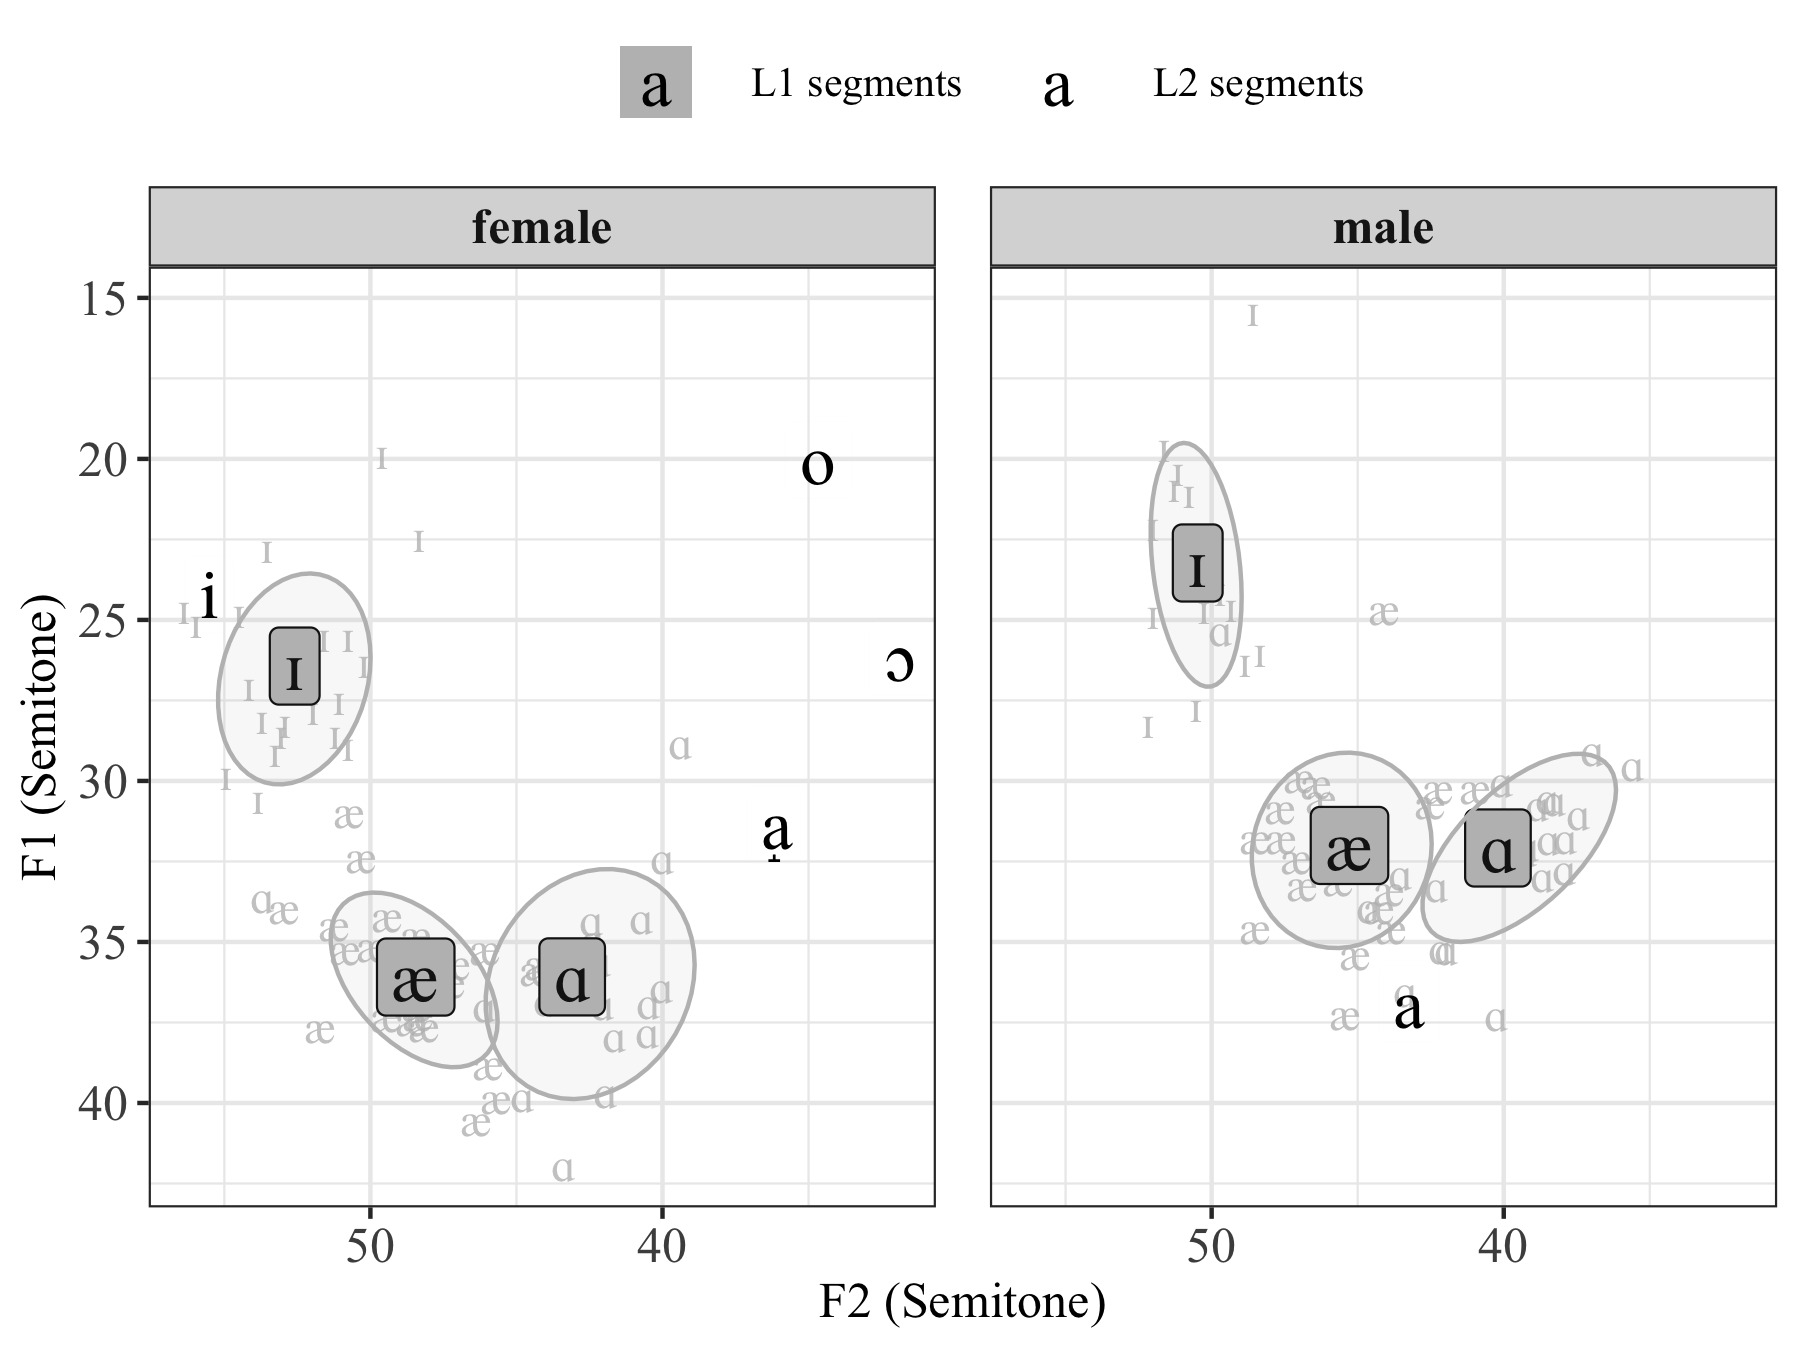
\includegraphics[width=0.7\textwidth]{figures/sup/smallplastic.png}
\end{figure}
\end{frame}
\subsection{Ratings}
\begin{frame}[shrink=30]
\frametitle{Experiment 2:  Rankings (Please call)}
\begin{columns}
\column{.55\textwidth}
   \begin{center}

\begin{tikzpicture}
  \begin{axis}[
  title={Mean Accentedness Ratings},
     % xbar,
   ytick={1,2,3,4,5,6,7,8,9},
     y=1cm,
  bar width=0.7 cm,
  xmin=0,
  xmax=7.5,
    axis y line*=left,
   axis x line=bottom,
    tickwidth         = 1pt,
    enlarge y limits  = 0.1,
    enlarge x limits  = 0.02,
  legend style={at={(1.2,0.55)},
  anchor=north},
  legend cell align=left,
      yticklabels from table={figures/bar2/data_plc.txt}{label},
      xtick distance=2,
      every axis plot/.append style={
          xbar,
          bar shift=0pt,
          fill
        }
    ]
\addplot [fill=red,color=mycolor3,select coords between index={0}{0}] table  [x=x,y=y] {figures/bar2/data_plc.txt};
\addplot [fill=red,color=mycolor1,select coords between index={1}{1}] table  [x=x,y=y] {figures/bar2/data_plc.txt};
\addplot [fill=blue,color=mycolor3,select coords between index={2}{9}] table [x=x, y=y] {figures/bar2/data_plc.txt};
 \addplot [color=black, only marks, mark=o]
 plot [error bars/.cd, x dir = both, x explicit]
 table[x =x, y =y, x error =err]{figures/bar2/data_plc.txt};
 \end{axis}
 \node[] at (7.50,8.7) {7.03};
\node[] at (6.83,7.7) {6.33};
\node[] at (5.98,6.7) {5.46};
\node[] at (5.69,5.7) {5.03};
\node[] at (5.53,4.7) {5.03};
\node[] at (5.23,3.7) {4.55};
\node[] at (4.60,2.7) {3.90};
\node[] at (4.35,1.7) {3.86};
\node[] at (4.39,0.7) {3.83};


\end{tikzpicture}

\end{center}
\column{.45\textwidth} 
\begin{center}
\textbf{Ranking 1:} \linebreak  \linebreak 
pʰl$\rightarrow$pl; pʰl$\rightarrow$pʰəl   \linebreak
$\Downarrow$ \linebreak
 z$\rightarrow$s; ɑ$\rightarrow$o  \linebreak
$\Downarrow$ \linebreak
ɑ$\rightarrow$ɔ; Match \linebreak\linebreak
\textbf{Ranking 2:}\linebreak \linebreak
pʰl$\rightarrow$pl \linebreak 
$\Downarrow$\linebreak 
kʰ$\rightarrow$k \linebreak
$\Downarrow$\linebreak 
ɑ$\rightarrow$ɔ; Match;pʰl$\rightarrow$pʰ; kʰɑl$\rightarrow$kʰɑ \linebreak\linebreak
\textbf{Ranking 3:}\linebreak \linebreak pʰl$\rightarrow$pʰəl; kʰ$\rightarrow$k \linebreak
$\Downarrow$\linebreak 
ɑ$\rightarrow$ɔ; Match; pʰl$\rightarrow$pʰ; kʰɑl$\rightarrow$kʰɑ\linebreak\linebreak
z$\rightarrow$s; ɑ$\rightarrow$o; kʰ$\rightarrow$k (No significant difference)
\end{center}
\end{columns}
\end{frame}
%--------------
\begin{frame}[shrink=30]
\frametitle{Experiment 2:  Rankings (Five Thick)}
\begin{columns}
\column{.55\textwidth}
   \begin{center}

\begin{tikzpicture}
  \begin{axis}[
  title={Mean Accentedness Ratings},
     % xbar,
   ytick={1,2,3,4,5,6,7,8,9},
     y=1cm,
  bar width=0.7 cm,
  xmin=0,
  xmax=7.5,
    axis y line*=left,
   axis x line=bottom,
    tickwidth         = 1pt,
    enlarge y limits  = 0.1,
    enlarge x limits  = 0.02,
  legend style={at={(1.2,0.55)},
  anchor=north},
  legend cell align=left,
      yticklabels from table={figures/bar2/data_fth.txt}{label},
      xtick distance=2,
      every axis plot/.append style={
          xbar,
          bar shift=0pt,
          fill
        }
    ]
\addplot [fill=red,color=mycolor3,select coords between index={0}{0}] table  [x=x,y=y] {figures/bar2/data_fth.txt};
\addplot [fill=red,color=mycolor1,select coords between index={1}{1}] table  [x=x,y=y] {figures/bar2/data_fth.txt};
\addplot [fill=blue,color=mycolor3,select coords between index={2}{9}] table [x=x, y=y] {figures/bar2/data_fth.txt};
 \addplot [color=black, only marks, mark=o]
 plot [error bars/.cd, x dir = both, x explicit]
 table[x =x, y =y, x error =err]{figures/bar2/data_fth.txt};
 \end{axis}
 \node[] at (6.91,8.7) {6.35};
\node[] at (6.75,7.7) {6.11};
\node[] at (6.67,6.7) {6.03};
\node[] at (5.93,5.7) {5.42};
\node[] at (6.01,4.7) {5.36};
\node[] at (5.65,3.7) {4.14};
\node[] at (5.62,2.7) {4.92};
\node[] at (4.92,1.7) {4.43};
\node[] at (4.91,0.7) {4.40};


\end{tikzpicture}

\end{center}
\column{.45\textwidth} 
\begin{center}
\textbf{Ranking 1:} \linebreak  \linebreak 
θ-> s̪t̪  \linebreak
$\Downarrow$\linebreak 
 faɪv$\rightarrow$faɪvə; θɪk$\rightarrow$θik \linebreak
$\Downarrow$\linebreak 
faɪv$\rightarrow$faɪ;  Match
 \linebreak\linebreak 
\textbf{Ranking 2:}\linebreak\linebreak
 θ-> s̪t̪ \linebreak
$\Downarrow$\linebreak 
faɪv$\rightarrow$faɪ; Match; θ$\rightarrow$f;  θ$\rightarrow$t̪\linebreak\linebreak 
\textbf{Ranking 3:} \linebreak\linebreak 
    aɪ$\rightarrow$ɑɪ; aɪ$\rightarrow$a \linebreak
$\Downarrow$\linebreak 
faɪv$\rightarrow$faɪ; Match; θ$\rightarrow$f\linebreak\linebreak 
aɪ$\rightarrow$ɑɪ; aɪ$\rightarrow$a; faɪv$\rightarrow$faɪvə; θɪk$\rightarrow$θik (no significant difference)
\end{center}
\end{columns}
\end{frame}
%-----------
\begin{frame}[shrink=30]
\frametitle{Experiment 2:  Rankings (Ask her)}
\begin{figure}
% Created by tikzDevice version 0.12.3 on 2019-11-27 22:20:10
% !TEX encoding = UTF-8 Unicode
\begin{tikzpicture}[x=1pt,y=1pt]
\definecolor{fillColor}{RGB}{255,255,255}
\path[use as bounding box,fill=fillColor,fill opacity=0.00] (0,0) rectangle (361.35,289.08);
\begin{scope}
\path[clip] (  0.00,  0.00) rectangle (361.35,289.08);
\definecolor{drawColor}{RGB}{255,255,255}
\definecolor{fillColor}{RGB}{255,255,255}

\path[draw=drawColor,line width= 0.6pt,line join=round,line cap=round,fill=fillColor] (  0.00, -0.00) rectangle (361.35,289.08);
\end{scope}
\begin{scope}
\path[clip] ( 31.71, 30.69) rectangle (188.36,227.94);
\definecolor{fillColor}{RGB}{255,255,255}

\path[fill=fillColor] ( 31.71, 30.69) rectangle (188.36,227.94);
\definecolor{drawColor}{gray}{0.92}

\path[draw=drawColor,line width= 0.3pt,line join=round] ( 31.71,210.99) --
	(188.36,210.99);

\path[draw=drawColor,line width= 0.3pt,line join=round] ( 31.71,155.86) --
	(188.36,155.86);

\path[draw=drawColor,line width= 0.3pt,line join=round] ( 31.71,100.73) --
	(188.36,100.73);

\path[draw=drawColor,line width= 0.3pt,line join=round] ( 31.71, 45.60) --
	(188.36, 45.60);

\path[draw=drawColor,line width= 0.3pt,line join=round] (161.67, 30.69) --
	(161.67,227.94);

\path[draw=drawColor,line width= 0.3pt,line join=round] (109.89, 30.69) --
	(109.89,227.94);

\path[draw=drawColor,line width= 0.3pt,line join=round] ( 58.12, 30.69) --
	( 58.12,227.94);

\path[draw=drawColor,line width= 0.6pt,line join=round] ( 31.71,183.43) --
	(188.36,183.43);

\path[draw=drawColor,line width= 0.6pt,line join=round] ( 31.71,128.30) --
	(188.36,128.30);

\path[draw=drawColor,line width= 0.6pt,line join=round] ( 31.71, 73.17) --
	(188.36, 73.17);

\path[draw=drawColor,line width= 0.6pt,line join=round] (187.56, 30.69) --
	(187.56,227.94);

\path[draw=drawColor,line width= 0.6pt,line join=round] (135.78, 30.69) --
	(135.78,227.94);

\path[draw=drawColor,line width= 0.6pt,line join=round] ( 84.01, 30.69) --
	( 84.01,227.94);

\path[draw=drawColor,line width= 0.6pt,line join=round] ( 32.23, 30.69) --
	( 32.23,227.94);
\definecolor{drawColor}{RGB}{190,190,190}

\node[text=drawColor,text opacity=0.80,anchor=base,inner sep=0pt, outer sep=0pt, scale=  1] at ( 88.36, 82.18) {æ};

\node[text=drawColor,text opacity=0.80,anchor=base,inner sep=0pt, outer sep=0pt, scale=  1] at (119.05, 83.77) {æ};

\node[text=drawColor,text opacity=0.80,anchor=base,inner sep=0pt, outer sep=0pt, scale=  1] at ( 69.43,125.41) {æ};

\node[text=drawColor,text opacity=0.80,anchor=base,inner sep=0pt, outer sep=0pt, scale=  1] at ( 67.90, 62.83) {æ};

\node[text=drawColor,text opacity=0.80,anchor=base,inner sep=0pt, outer sep=0pt, scale=  1] at ( 96.58,113.62) {æ};

\node[text=drawColor,text opacity=0.80,anchor=base,inner sep=0pt, outer sep=0pt, scale=  1] at (158.66, 60.49) {æ};

\node[text=drawColor,text opacity=0.80,anchor=base,inner sep=0pt, outer sep=0pt, scale=  1] at ( 88.18, 89.51) {æ};

\node[text=drawColor,text opacity=0.80,anchor=base,inner sep=0pt, outer sep=0pt, scale=  1] at ( 85.93,146.50) {æ};

\node[text=drawColor,text opacity=0.80,anchor=base,inner sep=0pt, outer sep=0pt, scale=  1] at ( 48.14,118.50) {æ};

\node[text=drawColor,text opacity=0.80,anchor=base,inner sep=0pt, outer sep=0pt, scale=  1] at ( 73.24, 78.02) {æ};

\node[text=drawColor,text opacity=0.80,anchor=base,inner sep=0pt, outer sep=0pt, scale=  1] at ( 96.62, 61.27) {æ};

\node[text=drawColor,text opacity=0.80,anchor=base,inner sep=0pt, outer sep=0pt, scale=  1] at ( 38.83,136.63) {æ};

\node[text=drawColor,text opacity=0.80,anchor=base,inner sep=0pt, outer sep=0pt, scale=  1] at (139.11, 95.45) {æ};

\node[text=drawColor,text opacity=0.80,anchor=base,inner sep=0pt, outer sep=0pt, scale=  1] at ( 81.15, 85.15) {æ};

\node[text=drawColor,text opacity=0.80,anchor=base,inner sep=0pt, outer sep=0pt, scale=  1] at (135.12, 76.09) {æ};

\node[text=drawColor,text opacity=0.80,anchor=base,inner sep=0pt, outer sep=0pt, scale=  1] at ( 75.22, 88.11) {æ};

\node[text=drawColor,text opacity=0.80,anchor=base,inner sep=0pt, outer sep=0pt, scale=  1] at ( 51.03,146.62) {æ};

\node[text=drawColor,text opacity=0.80,anchor=base,inner sep=0pt, outer sep=0pt, scale=  1] at ( 78.29, 98.10) {æ};

\node[text=drawColor,text opacity=0.80,anchor=base,inner sep=0pt, outer sep=0pt, scale=  1] at ( 67.29,120.22) {æ};

\node[text=drawColor,text opacity=0.80,anchor=base,inner sep=0pt, outer sep=0pt, scale=  1] at ( 56.53,101.16) {æ};

\node[text=drawColor,text opacity=0.80,anchor=base,inner sep=0pt, outer sep=0pt, scale=  1] at ( 82.18, 60.58) {æ};

\node[text=drawColor,text opacity=0.80,anchor=base,inner sep=0pt, outer sep=0pt, scale=  1] at (133.04,101.85) {æ};

\node[text=drawColor,text opacity=0.80,anchor=base,inner sep=0pt, outer sep=0pt, scale=  1] at ( 84.20, 95.50) {æ};

\node[text=drawColor,text opacity=0.80,anchor=base,inner sep=0pt, outer sep=0pt, scale=  1] at (110.70, 35.73) {æ};

\node[text=drawColor,text opacity=0.80,anchor=base,inner sep=0pt, outer sep=0pt, scale=  1] at ( 70.46,140.31) {æ};

\node[text=drawColor,text opacity=0.80,anchor=base,inner sep=0pt, outer sep=0pt, scale=  1] at (103.29,103.13) {æ};
\definecolor{drawColor}{RGB}{0,0,0}
\definecolor{fillColor}{RGB}{190,190,190}

\path[draw=drawColor,line width= 0.3pt,line join=round,line cap=round,fill=fillColor] ( 82.93, 91.44) --
	( 93.88, 91.44) --
	( 93.80, 91.44) --
	( 94.09, 91.46) --
	( 94.38, 91.51) --
	( 94.65, 91.62) --
	( 94.90, 91.76) --
	( 95.13, 91.95) --
	( 95.32, 92.16) --
	( 95.48, 92.41) --
	( 95.59, 92.68) --
	( 95.66, 92.96) --
	( 95.68, 93.25) --
	( 95.68, 93.25) --
	( 95.68,107.41) --
	( 95.68,107.41) --
	( 95.66,107.70) --
	( 95.59,107.99) --
	( 95.48,108.25) --
	( 95.32,108.50) --
	( 95.13,108.72) --
	( 94.90,108.90) --
	( 94.65,109.05) --
	( 94.38,109.15) --
	( 94.09,109.21) --
	( 93.88,109.22) --
	( 82.93,109.22) --
	( 83.15,109.21) --
	( 82.86,109.22) --
	( 82.57,109.18) --
	( 82.29,109.10) --
	( 82.03,108.98) --
	( 81.79,108.81) --
	( 81.58,108.61) --
	( 81.41,108.38) --
	( 81.27,108.12) --
	( 81.18,107.85) --
	( 81.13,107.56) --
	( 81.13,107.41) --
	( 81.13, 93.25) --
	( 81.13, 93.39) --
	( 81.13, 93.10) --
	( 81.18, 92.82) --
	( 81.27, 92.54) --
	( 81.41, 92.28) --
	( 81.58, 92.05) --
	( 81.79, 91.85) --
	( 82.03, 91.68) --
	( 82.29, 91.56) --
	( 82.57, 91.48) --
	( 82.86, 91.44) --
	cycle;
\end{scope}
\begin{scope}
\path[clip] ( 31.71, 30.69) rectangle (188.36,227.94);
\definecolor{drawColor}{RGB}{0,0,0}

\node[text=drawColor,anchor=base,inner sep=0pt, outer sep=0pt, scale=  1.50] at ( 88.41, 94.45) {æ};

%\path[draw=drawColor,line width= 0.0pt,line join=round,line cap=round] (129.65,120.66) --
	(150.07,120.66) --
	(150.00,120.66) --
	(150.29,120.67) --
	(150.57,120.73) --
	(150.84,120.83) --
	(151.10,120.98) --
	(151.32,121.16) --
	(151.51,121.38) --
	(151.67,121.63) --
	(151.78,121.89) --
	(151.85,122.18) --
	(151.88,122.47) --
	(151.88,122.47) --
	(151.88,136.63) --
	(151.88,136.63) --
	(151.85,136.92) --
	(151.78,137.20) --
	(151.67,137.47) --
	(151.51,137.72) --
	(151.32,137.94) --
	(151.10,138.12) --
	(150.84,138.26) --
	(150.57,138.37) --
	(150.29,138.43) --
	(150.07,138.44) --
	(129.65,138.44) --
	(129.86,138.43) --
	(129.57,138.44) --
	(129.29,138.40) --
	(129.01,138.32) --
	(128.74,138.20) --
	(128.50,138.03) --
	(128.29,137.83) --
	(128.12,137.60) --
	(127.98,137.34) --
	(127.89,137.06) --
	(127.85,136.78) --
	(127.84,136.63) --
	(127.84,122.47) --
	(127.85,122.61) --
	(127.85,122.32) --
	(127.89,122.03) --
	(127.98,121.76) --
	(128.12,121.50) --
	(128.29,121.27) --
	(128.50,121.07) --
	(128.74,120.90) --
	(129.01,120.78) --
	(129.29,120.70) --
	(129.57,120.66) --
	(129.65,120.66);
\end{scope}
\begin{scope}
\path[clip] ( 31.71, 30.69) rectangle (188.36,227.94);
\definecolor{drawColor}{RGB}{0,0,0}

\node[text=drawColor,anchor=base,inner sep=0pt, outer sep=0pt, scale=  1.50] at (139.86,123.67) {a};
\definecolor{drawColor}{RGB}{190,190,190}
\definecolor{fillColor}{RGB}{190,190,190}

\path[draw=drawColor,line width= 0.6pt,line join=round,line cap=round,fill=fillColor,fill opacity=0.10] (124.90, 82.34) --
	(124.61, 86.71) --
	(123.73, 91.28) --
	(122.27, 96.00) --
	(120.26,100.78) --
	(117.73,105.57) --
	(114.72,110.28) --
	(111.28,114.84) --
	(107.44,119.19) --
	(103.29,123.26) --
	( 98.86,126.98) --
	( 94.24,130.31) --
	( 89.50,133.18) --
	( 84.70,135.57) --
	( 79.92,137.42) --
	( 75.23,138.72) --
	( 70.70,139.44) --
	( 66.40,139.57) --
	( 62.40,139.11) --
	( 58.75,138.07) --
	( 55.51,136.46) --
	( 52.74,134.31) --
	( 50.47,131.65) --
	( 48.73,128.51) --
	( 47.56,124.96) --
	( 46.97,121.04) --
	( 46.97,116.81) --
	( 47.56,112.33) --
	( 48.73,107.68) --
	( 50.47,102.92) --
	( 52.74, 98.12) --
	( 55.51, 93.37) --
	( 58.75, 88.72) --
	( 62.40, 84.26) --
	( 66.40, 80.04) --
	( 70.70, 76.14) --
	( 75.23, 72.60) --
	( 79.92, 69.50) --
	( 84.70, 66.86) --
	( 89.50, 64.74) --
	( 94.24, 63.16) --
	( 98.86, 62.15) --
	(103.29, 61.73) --
	(107.44, 61.89) --
	(111.28, 62.64) --
	(114.72, 63.97) --
	(117.73, 65.85) --
	(120.26, 68.26) --
	(122.27, 71.17) --
	(123.73, 74.51) --
	(124.61, 78.26) --
	(124.90, 82.34) --
	cycle;
\definecolor{drawColor}{gray}{0.20}

\path[draw=drawColor,line width= 0.6pt,line join=round,line cap=round] ( 31.71, 30.69) rectangle (188.36,227.94);
\end{scope}
\begin{scope}
\path[clip] (199.20, 30.69) rectangle (355.85,227.94);
\definecolor{fillColor}{RGB}{255,255,255}

\path[fill=fillColor] (199.20, 30.69) rectangle (355.85,227.94);
\definecolor{drawColor}{gray}{0.92}

\path[draw=drawColor,line width= 0.3pt,line join=round] (199.20,210.99) --
	(355.85,210.99);

\path[draw=drawColor,line width= 0.3pt,line join=round] (199.20,155.86) --
	(355.85,155.86);

\path[draw=drawColor,line width= 0.3pt,line join=round] (199.20,100.73) --
	(355.85,100.73);

\path[draw=drawColor,line width= 0.3pt,line join=round] (199.20, 45.60) --
	(355.85, 45.60);

\path[draw=drawColor,line width= 0.3pt,line join=round] (329.16, 30.69) --
	(329.16,227.94);

\path[draw=drawColor,line width= 0.3pt,line join=round] (277.38, 30.69) --
	(277.38,227.94);

\path[draw=drawColor,line width= 0.3pt,line join=round] (225.61, 30.69) --
	(225.61,227.94);

\path[draw=drawColor,line width= 0.6pt,line join=round] (199.20,183.43) --
	(355.85,183.43);

\path[draw=drawColor,line width= 0.6pt,line join=round] (199.20,128.30) --
	(355.85,128.30);

\path[draw=drawColor,line width= 0.6pt,line join=round] (199.20, 73.17) --
	(355.85, 73.17);

\path[draw=drawColor,line width= 0.6pt,line join=round] (355.05, 30.69) --
	(355.05,227.94);

\path[draw=drawColor,line width= 0.6pt,line join=round] (303.27, 30.69) --
	(303.27,227.94);

\path[draw=drawColor,line width= 0.6pt,line join=round] (251.50, 30.69) --
	(251.50,227.94);

\path[draw=drawColor,line width= 0.6pt,line join=round] (199.72, 30.69) --
	(199.72,227.94);
\definecolor{drawColor}{RGB}{190,190,190}

\node[text=drawColor,text opacity=0.80,anchor=base,inner sep=0pt, outer sep=0pt, scale=  1] at (280.82,106.95) {æ};

\node[text=drawColor,text opacity=0.80,anchor=base,inner sep=0pt, outer sep=0pt, scale=  1] at (268.78,142.15) {æ};

\node[text=drawColor,text opacity=0.80,anchor=base,inner sep=0pt, outer sep=0pt, scale=  1] at (279.30,137.08) {æ};

\node[text=drawColor,text opacity=0.80,anchor=base,inner sep=0pt, outer sep=0pt, scale=  1] at (253.45,174.49) {æ};

\node[text=drawColor,text opacity=0.80,anchor=base,inner sep=0pt, outer sep=0pt, scale=  1] at (259.66,174.98) {æ};

\node[text=drawColor,text opacity=0.80,anchor=base,inner sep=0pt, outer sep=0pt, scale=  1] at (259.92,156.12) {æ};

\node[text=drawColor,text opacity=0.80,anchor=base,inner sep=0pt, outer sep=0pt, scale=  1] at (322.06,126.68) {æ};

\node[text=drawColor,text opacity=0.80,anchor=base,inner sep=0pt, outer sep=0pt, scale=  1] at (275.24,167.24) {æ};

\node[text=drawColor,text opacity=0.80,anchor=base,inner sep=0pt, outer sep=0pt, scale=  1] at (283.61,160.74) {æ};

\node[text=drawColor,text opacity=0.80,anchor=base,inner sep=0pt, outer sep=0pt, scale=  1] at (276.49,121.97) {æ};

\node[text=drawColor,text opacity=0.80,anchor=base,inner sep=0pt, outer sep=0pt, scale=  1] at (257.60,215.05) {æ};

\node[text=drawColor,text opacity=0.80,anchor=base,inner sep=0pt, outer sep=0pt, scale=  1] at (278.70,162.71) {æ};

\node[text=drawColor,text opacity=0.80,anchor=base,inner sep=0pt, outer sep=0pt, scale=  1] at (254.10,140.42) {æ};

\node[text=drawColor,text opacity=0.80,anchor=base,inner sep=0pt, outer sep=0pt, scale=  1] at (286.59,139.41) {æ};

\node[text=drawColor,text opacity=0.80,anchor=base,inner sep=0pt, outer sep=0pt, scale=  1] at (270.48,152.24) {æ};

\node[text=drawColor,text opacity=0.80,anchor=base,inner sep=0pt, outer sep=0pt, scale=  1] at (291.49,150.07) {æ};

\node[text=drawColor,text opacity=0.80,anchor=base,inner sep=0pt, outer sep=0pt, scale=  1] at (251.12, 81.44) {æ};

\node[text=drawColor,text opacity=0.80,anchor=base,inner sep=0pt, outer sep=0pt, scale=  1] at (280.24,133.80) {æ};

\node[text=drawColor,text opacity=0.80,anchor=base,inner sep=0pt, outer sep=0pt, scale=  1] at (279.36,123.50) {æ};

\node[text=drawColor,text opacity=0.80,anchor=base,inner sep=0pt, outer sep=0pt, scale=  1] at (272.80,214.75) {æ};

\node[text=drawColor,text opacity=0.80,anchor=base,inner sep=0pt, outer sep=0pt, scale=  1] at (262.69,176.28) {æ};
\definecolor{drawColor}{RGB}{0,0,0}
\definecolor{fillColor}{RGB}{190,190,190}

\path[draw=drawColor,line width= 0.3pt,line join=round,line cap=round,fill=fillColor] (268.08,145.41) --
	(279.02,145.41) --
	(278.95,145.42) --
	(279.24,145.43) --
	(279.52,145.49) --
	(279.79,145.59) --
	(280.05,145.73) --
	(280.27,145.92) --
	(280.46,146.14) --
	(280.62,146.38) --
	(280.73,146.65) --
	(280.80,146.93) --
	(280.83,147.22) --
	(280.83,147.22) --
	(280.83,161.39) --
	(280.83,161.39) --
	(280.80,161.68) --
	(280.73,161.96) --
	(280.62,162.23) --
	(280.46,162.47) --
	(280.27,162.69) --
	(280.05,162.87) --
	(279.79,163.02) --
	(279.52,163.12) --
	(279.24,163.18) --
	(279.02,163.19) --
	(268.08,163.19) --
	(268.29,163.18) --
	(268.00,163.19) --
	(267.72,163.16) --
	(267.44,163.08) --
	(267.17,162.95) --
	(266.93,162.79) --
	(266.72,162.59) --
	(266.55,162.35) --
	(266.41,162.10) --
	(266.32,161.82) --
	(266.28,161.53) --
	(266.27,161.39) --
	(266.27,147.22) --
	(266.28,147.37) --
	(266.28,147.08) --
	(266.32,146.79) --
	(266.41,146.51) --
	(266.55,146.26) --
	(266.72,146.02) --
	(266.93,145.82) --
	(267.17,145.66) --
	(267.44,145.53) --
	(267.72,145.45) --
	(268.00,145.42) --
	cycle;
\end{scope}
\begin{scope}
\path[clip] (199.20, 30.69) rectangle (355.85,227.94);
\definecolor{drawColor}{RGB}{0,0,0}

\node[text=drawColor,anchor=base,inner sep=0pt, outer sep=0pt, scale=  1.50] at (273.55,148.43) {æ};

%\path[draw=drawColor,line width= 0.0pt,line join=round,line cap=round] (310.40,148.34) --
	(330.83,148.34) --
	(330.76,148.34) --
	(331.05,148.35) --
	(331.33,148.41) --
	(331.60,148.51) --
	(331.85,148.66) --
	(332.08,148.84) --
	(332.27,149.06) --
	(332.43,149.31) --
	(332.54,149.57) --
	(332.61,149.85) --
	(332.63,150.14) --
	(332.63,150.14) --
	(332.63,164.31) --
	(332.63,164.31) --
	(332.61,164.60) --
	(332.54,164.88) --
	(332.43,165.15) --
	(332.27,165.40) --
	(332.08,165.61) --
	(331.85,165.80) --
	(331.60,165.94) --
	(331.33,166.05) --
	(331.05,166.10) --
	(330.83,166.12) --
	(310.40,166.12) --
	(310.62,166.10) --
	(310.33,166.12) --
	(310.04,166.08) --
	(309.76,166.00) --
	(309.50,165.87) --
	(309.26,165.71) --
	(309.05,165.51) --
	(308.88,165.28) --
	(308.74,165.02) --
	(308.65,164.74) --
	(308.60,164.46) --
	(308.60,164.31) --
	(308.60,150.14) --
	(308.60,150.29) --
	(308.60,150.00) --
	(308.65,149.71) --
	(308.74,149.44) --
	(308.88,149.18) --
	(309.05,148.95) --
	(309.26,148.75) --
	(309.50,148.58) --
	(309.76,148.46) --
	(310.04,148.37) --
	(310.33,148.34) --
	(310.40,148.34);
\end{scope}
\begin{scope}
\path[clip] (199.20, 30.69) rectangle (355.85,227.94);
\definecolor{drawColor}{RGB}{0,0,0}

\node[text=drawColor,anchor=base,inner sep=0pt, outer sep=0pt, scale=  1.50] at (320.62,151.35) {a};

%\path[draw=drawColor,line width= 0.0pt,line join=round,line cap=round] (316.13, 96.67) --
	(331.81, 96.67) --
	(331.74, 96.67) --
	(332.03, 96.68) --
	(332.31, 96.74) --
	(332.58, 96.84) --
	(332.83, 96.99) --
	(333.06, 97.17) --
	(333.25, 97.39) --
	(333.41, 97.64) --
	(333.52, 97.90) --
	(333.59, 98.19) --
	(333.62, 98.48) --
	(333.62, 98.48) --
	(333.62,112.64) --
	(333.62,112.64) --
	(333.59,112.93) --
	(333.52,113.21) --
	(333.41,113.48) --
	(333.25,113.73) --
	(333.06,113.94) --
	(332.83,114.13) --
	(332.58,114.27) --
	(332.31,114.38) --
	(332.03,114.43) --
	(331.81,114.45) --
	(316.13,114.45) --
	(316.34,114.43) --
	(316.05,114.45) --
	(315.76,114.41) --
	(315.49,114.33) --
	(315.22,114.21) --
	(314.98,114.04) --
	(314.77,113.84) --
	(314.60,113.61) --
	(314.46,113.35) --
	(314.37,113.07) --
	(314.33,112.79) --
	(314.32,112.64) --
	(314.32, 98.48) --
	(314.33, 98.62) --
	(314.33, 98.33) --
	(314.37, 98.04) --
	(314.46, 97.77) --
	(314.60, 97.51) --
	(314.77, 97.28) --
	(314.98, 97.08) --
	(315.22, 96.91) --
	(315.49, 96.79) --
	(315.76, 96.71) --
	(316.05, 96.67) --
	(316.13, 96.67);
\end{scope}
\begin{scope}
\path[clip] (199.20, 30.69) rectangle (355.85,227.94);
\definecolor{drawColor}{RGB}{0,0,0}

\node[text=drawColor,anchor=base,inner sep=0pt, outer sep=0pt, scale=  1.50] at (323.97, 99.68) {æ̞};

%\path[draw=drawColor,line width= 0.0pt,line join=round,line cap=round] (275.20,169.29) --
	(295.62,169.29) --
	(295.55,169.29) --
	(295.84,169.30) --
	(296.13,169.36) --
	(296.40,169.46) --
	(296.65,169.61) --
	(296.88,169.79) --
	(297.07,170.01) --
	(297.22,170.25) --
	(297.34,170.52) --
	(297.41,170.80) --
	(297.43,171.09) --
	(297.43,171.09) --
	(297.43,185.26) --
	(297.43,185.26) --
	(297.41,185.55) --
	(297.34,185.83) --
	(297.22,186.10) --
	(297.07,186.34) --
	(296.88,186.56) --
	(296.65,186.75) --
	(296.40,186.89) --
	(296.13,186.99) --
	(295.84,187.05) --
	(295.62,187.07) --
	(275.20,187.07) --
	(275.42,187.05) --
	(275.13,187.06) --
	(274.84,187.03) --
	(274.56,186.95) --
	(274.30,186.82) --
	(274.06,186.66) --
	(273.85,186.46) --
	(273.67,186.22) --
	(273.54,185.97) --
	(273.45,185.69) --
	(273.40,185.40) --
	(273.39,185.26) --
	(273.39,171.09) --
	(273.40,171.24) --
	(273.40,170.95) --
	(273.45,170.66) --
	(273.54,170.39) --
	(273.67,170.13) --
	(273.85,169.90) --
	(274.06,169.69) --
	(274.30,169.53) --
	(274.56,169.40) --
	(274.84,169.32) --
	(275.13,169.29) --
	(275.20,169.29);
\end{scope}
\begin{scope}
\path[clip] (199.20, 30.69) rectangle (355.85,227.94);
\definecolor{drawColor}{RGB}{0,0,0}

\node[text=drawColor,anchor=base,inner sep=0pt, outer sep=0pt, scale=  1.50] at (285.41,172.30) {æ̝};

%\path[draw=drawColor,line width= 0.0pt,line join=round,line cap=round] (338.52,136.60) --
	(358.94,136.60) --
	(358.87,136.60) --
	(359.16,136.61) --
	(359.44,136.67) --
	(359.72,136.77) --
	(359.97,136.92) --
	(360.19,137.10) --
	(360.39,137.32) --
	(360.54,137.57) --
	(360.65,137.83) --
	(360.72,138.12) --
	(360.75,138.41) --
	(360.75,138.41) --
	(360.75,152.57) --
	(360.75,152.57) --
	(360.72,152.86) --
	(360.65,153.14) --
	(360.54,153.41) --
	(360.39,153.66) --
	(360.19,153.87) --
	(359.97,154.06) --
	(359.72,154.20) --
	(359.44,154.31) --
	(359.16,154.36) --
	(358.94,154.38) --
	(338.52,154.38) --
	(338.74,154.36) --
	(338.45,154.38) --
	(338.16,154.34) --
	(337.88,154.26) --
	(337.61,154.14) --
	(337.38,153.97) --
	(337.17,153.77) --
	(336.99,153.54) --
	(336.86,153.28) --
	(336.76,153.00) --
	(336.72,152.72) --
	(336.71,152.57) --
	(336.71,138.41) --
	(336.72,138.55) --
	(336.72,138.26) --
	(336.76,137.97) --
	(336.86,137.70) --
	(336.99,137.44) --
	(337.17,137.21) --
	(337.38,137.01) --
	(337.61,136.84) --
	(337.88,136.72) --
	(338.16,136.64) --
	(338.45,136.60) --
	(338.52,136.60);
\end{scope}
\begin{scope}
\path[clip] (199.20, 30.69) rectangle (355.85,227.94);
\definecolor{drawColor}{RGB}{0,0,0}

\node[text=drawColor,anchor=base,inner sep=0pt, outer sep=0pt, scale=  1.50] at (348.73,139.61) {ɑ};
\definecolor{drawColor}{RGB}{190,190,190}
\definecolor{fillColor}{RGB}{190,190,190}

\path[draw=drawColor,line width= 0.6pt,line join=round,line cap=round,fill=fillColor,fill opacity=0.10] (292.39,141.61) --
	(292.25,146.23) --
	(291.82,150.98) --
	(291.10,155.78) --
	(290.12,160.57) --
	(288.89,165.27) --
	(287.42,169.81) --
	(285.74,174.13) --
	(283.86,178.14) --
	(281.83,181.81) --
	(279.67,185.06) --
	(277.42,187.85) --
	(275.10,190.15) --
	(272.76,191.90) --
	(270.42,193.09) --
	(268.13,193.70) --
	(265.92,193.72) --
	(263.82,193.15) --
	(261.87,191.99) --
	(260.08,190.27) --
	(258.50,188.01) --
	(257.15,185.25) --
	(256.04,182.03) --
	(255.19,178.39) --
	(254.62,174.39) --
	(254.33,170.09) --
	(254.33,165.56) --
	(254.62,160.87) --
	(255.19,156.08) --
	(256.04,151.28) --
	(257.15,146.52) --
	(258.50,141.89) --
	(260.08,137.46) --
	(261.87,133.28) --
	(263.82,129.43) --
	(265.92,125.97) --
	(268.13,122.94) --
	(270.42,120.39) --
	(272.76,118.37) --
	(275.10,116.89) --
	(277.42,115.99) --
	(279.67,115.68) --
	(281.83,115.95) --
	(283.86,116.82) --
	(285.74,118.26) --
	(287.42,120.25) --
	(288.89,122.77) --
	(290.12,125.77) --
	(291.10,129.21) --
	(291.82,133.03) --
	(292.25,137.19) --
	(292.39,141.61) --
	cycle;
\definecolor{drawColor}{gray}{0.20}

\path[draw=drawColor,line width= 0.6pt,line join=round,line cap=round] (199.20, 30.69) rectangle (355.85,227.94);
\end{scope}
\begin{scope}
\path[clip] ( 31.71,227.94) rectangle (188.36,244.51);
\definecolor{drawColor}{gray}{0.20}
\definecolor{fillColor}{gray}{0.85}

\path[draw=drawColor,line width= 0.6pt,line join=round,line cap=round,fill=fillColor] ( 31.71,227.94) rectangle (188.36,244.51);
\definecolor{drawColor}{gray}{0.10}

\node[text=drawColor,anchor=base,inner sep=0pt, outer sep=0pt, scale=  1] at (110.04,233.19) {female};
\end{scope}
\begin{scope}
\path[clip] (199.20,227.94) rectangle (355.85,244.51);
\definecolor{drawColor}{gray}{0.20}
\definecolor{fillColor}{gray}{0.85}

\path[draw=drawColor,line width= 0.6pt,line join=round,line cap=round,fill=fillColor] (199.20,227.94) rectangle (355.85,244.51);
\definecolor{drawColor}{gray}{0.10}

\node[text=drawColor,anchor=base,inner sep=0pt, outer sep=0pt, scale=  1] at (277.53,233.19) {male};
\end{scope}
\begin{scope}
\path[clip] (  0.00,  0.00) rectangle (361.35,289.08);
\definecolor{drawColor}{gray}{0.20}

\path[draw=drawColor,line width= 0.6pt,line join=round] (187.56, 27.94) --
	(187.56, 30.69);

\path[draw=drawColor,line width= 0.6pt,line join=round] (135.78, 27.94) --
	(135.78, 30.69);

\path[draw=drawColor,line width= 0.6pt,line join=round] ( 84.01, 27.94) --
	( 84.01, 30.69);

\path[draw=drawColor,line width= 0.6pt,line join=round] ( 32.23, 27.94) --
	( 32.23, 30.69);
\end{scope}
\begin{scope}
\path[clip] (  0.00,  0.00) rectangle (361.35,289.08);
\definecolor{drawColor}{gray}{0.30}

\node[text=drawColor,anchor=base,inner sep=0pt, outer sep=0pt, scale=  0.88] at (187.56, 19.68) {40};

\node[text=drawColor,anchor=base,inner sep=0pt, outer sep=0pt, scale=  0.88] at (135.78, 19.68) {45};

\node[text=drawColor,anchor=base,inner sep=0pt, outer sep=0pt, scale=  0.88] at ( 84.01, 19.68) {50};

\node[text=drawColor,anchor=base,inner sep=0pt, outer sep=0pt, scale=  0.88] at ( 32.23, 19.68) {55};
\end{scope}
\begin{scope}
\path[clip] (  0.00,  0.00) rectangle (361.35,289.08);
\definecolor{drawColor}{gray}{0.20}

\path[draw=drawColor,line width= 0.6pt,line join=round] (355.05, 27.94) --
	(355.05, 30.69);

\path[draw=drawColor,line width= 0.6pt,line join=round] (303.27, 27.94) --
	(303.27, 30.69);

\path[draw=drawColor,line width= 0.6pt,line join=round] (251.50, 27.94) --
	(251.50, 30.69);

\path[draw=drawColor,line width= 0.6pt,line join=round] (199.72, 27.94) --
	(199.72, 30.69);
\end{scope}
\begin{scope}
\path[clip] (  0.00,  0.00) rectangle (361.35,289.08);
\definecolor{drawColor}{gray}{0.30}

\node[text=drawColor,anchor=base,inner sep=0pt, outer sep=0pt, scale=  0.88] at (355.05, 19.68) {40};

\node[text=drawColor,anchor=base,inner sep=0pt, outer sep=0pt, scale=  0.88] at (303.27, 19.68) {45};

\node[text=drawColor,anchor=base,inner sep=0pt, outer sep=0pt, scale=  0.88] at (251.50, 19.68) {50};

\node[text=drawColor,anchor=base,inner sep=0pt, outer sep=0pt, scale=  0.88] at (199.72, 19.68) {55};
\end{scope}
\begin{scope}
\path[clip] (  0.00,  0.00) rectangle (361.35,289.08);
\definecolor{drawColor}{gray}{0.30}

\node[text=drawColor,anchor=base east,inner sep=0pt, outer sep=0pt, scale=  0.88] at ( 26.76,180.40) {30};

\node[text=drawColor,anchor=base east,inner sep=0pt, outer sep=0pt, scale=  0.88] at ( 26.76,125.27) {35};

\node[text=drawColor,anchor=base east,inner sep=0pt, outer sep=0pt, scale=  0.88] at ( 26.76, 70.14) {40};
\end{scope}
\begin{scope}
\path[clip] (  0.00,  0.00) rectangle (361.35,289.08);
\definecolor{drawColor}{gray}{0.20}

\path[draw=drawColor,line width= 0.6pt,line join=round] ( 28.96,183.43) --
	( 31.71,183.43);

\path[draw=drawColor,line width= 0.6pt,line join=round] ( 28.96,128.30) --
	( 31.71,128.30);

\path[draw=drawColor,line width= 0.6pt,line join=round] ( 28.96, 73.17) --
	( 31.71, 73.17);
\end{scope}
\begin{scope}
\path[clip] (  0.00,  0.00) rectangle (361.35,289.08);
\definecolor{drawColor}{RGB}{0,0,0}

\node[text=drawColor,anchor=base,inner sep=0pt, outer sep=0pt, scale=  1] at (193.78,  7.64) {F2 (Semitone)};
\end{scope}
\begin{scope}
\path[clip] (  0.00,  0.00) rectangle (361.35,289.08);
\definecolor{drawColor}{RGB}{0,0,0}

\node[text=drawColor,rotate= 90.00,anchor=base,inner sep=0pt, outer sep=0pt, scale=  1] at ( 13.08,129.31) {F1 (Semitone)};
\end{scope}
\begin{scope}
\path[clip] (  0.00,  0.00) rectangle (361.35,289.08);
\definecolor{fillColor}{RGB}{255,255,255}

\path[fill=fillColor] ( 95.37,255.51) rectangle (292.19,283.58);
\end{scope}
\begin{scope}
\path[clip] (  0.00,  0.00) rectangle (361.35,289.08);
\definecolor{fillColor}{RGB}{255,255,255}

\path[fill=fillColor] (115.10,261.01) rectangle (132.17,278.08);
\end{scope}
\begin{scope}
\path[clip] (  0.00,  0.00) rectangle (361.35,289.08);
\definecolor{fillColor}{RGB}{190,190,190}

\path[fill=fillColor] (115.10,261.01) rectangle (132.17,276.08);
\definecolor{drawColor}{RGB}{0,0,0}

\node[text=drawColor,anchor=base,inner sep=0pt, outer sep=0pt, scale=  1.50] at (123.63,263.67) {æ};
\end{scope}
\begin{scope}
\path[clip] (  0.00,  0.00) rectangle (361.35,289.08);
\definecolor{fillColor}{RGB}{255,255,255}

\path[fill=fillColor] (208.01,261.01) rectangle (225.08,278.08);
\end{scope}
\begin{scope}
\path[clip] (  0.00,  0.00) rectangle (361.35,289.08);

\path[] (208.01,261.01) rectangle (225.08,278.08);
\definecolor{drawColor}{RGB}{0,0,0}

\node[text=drawColor,anchor=base,inner sep=0pt, outer sep=0pt, scale=  1.50] at (216.54,263.67) {æ};
\end{scope}
\begin{scope}
\path[clip] (  0.00,  0.00) rectangle (361.35,289.08);
\definecolor{drawColor}{RGB}{0,0,0}

\node[text=drawColor,anchor=base west,inner sep=0pt, outer sep=0pt, scale=  1] at (146.39,263.67) {L1 segments};
\end{scope}
\begin{scope}
\path[clip] (  0.00,  0.00) rectangle (361.35,289.08);
\definecolor{drawColor}{RGB}{0,0,0}

\node[text=drawColor,anchor=base west,inner sep=0pt, outer sep=0pt, scale=  1] at (235.31,263.67) {L2 segments};
\end{scope}
\end{tikzpicture}

\end{figure}
\end{frame}
%-----------
\begin{frame}[shrink=25]
\frametitle{Experiment 2:  Rankings (Small plastic)}
\begin{figure}

\begin{tikzpicture}
  \begin{axis}[
  title={Mean Accentedness Ratings},
     % xbar,
   ytick={1,2,3,4,5,6,7,8,9,10,11},
     y=1cm,
  bar width=0.7 cm,
  xmin=0,
  xmax=7.5,
    axis y line*=left,
   axis x line=bottom,
    tickwidth         = 1pt,
    enlarge y limits  = 0.1,
    enlarge x limits  = 0.02,
  legend style={at={(1.2,0.55)},
  anchor=north},
  legend cell align=left,
      yticklabels from table={figures/bar2/data_smp.txt}{label},
      xtick distance=2,
      every axis plot/.append style={
          xbar,
          bar shift=0pt,
          fill
        }
    ]
\addplot [fill=red,color=mycolor3,select coords between index={0}{1}] table  [x=x,y=y] {figures/bar2/data_smp.txt};
\addplot [fill=red,color=mycolor1,select coords between index={2}{2}] table  [x=x,y=y] {figures/bar2/data_smp.txt};
\addplot [fill=blue,color=mycolor3,select coords between index={3}{11}] table [x=x, y=y] {figures/bar2/data_smp.txt};
 \addplot [color=black, only marks, mark=o]
 plot [error bars/.cd, x dir = both, x explicit]
 table[x =x, y =y, x error =err]{figures/bar2/data_smp.txt};
 \end{axis}
 \node[] at (7.23,11) {6.61};
\node[] at (7.11,10) {6.48};
\node[] at (6.75,9) {6.14};
\node[] at (6.20,8) {5.61};
\node[] at (5.91,7) {5.36};
\node[] at (5.70,6) {5.24};
\node[] at (5.80,5) {5.15};
\node[] at (5.61,4) {4.96};
\node[] at (5.31,3) {4.85};
\node[] at (5.26,2) {4.60};
\node[] at (5.07,1) {4.42};


\end{tikzpicture}

\end{figure}
\end{frame}
%------------
\begin{frame}[shrink=25]
\frametitle{Experiment 2:  Rankings (Six spoons)}
\begin{figure}

\begin{tikzpicture}
  \begin{axis}[
  title={Mean Accentedness Ratings},
     % xbar,
   ytick={1,2,3,4,5,6,7,8},
     y=1cm,
  bar width=0.7 cm,
  xmin=0,
  xmax=7.1,
    axis y line*=left,
   axis x line=bottom,
    tickwidth         = 1pt,
    enlarge y limits  = 0.1,
    enlarge x limits  = 0.02,
  legend style={at={(1.2,0.55)},
  anchor=north},
  legend cell align=left,
      yticklabels from table={figures/sup/data_ssp.txt}{label},
      xtick distance=2,
      every axis plot/.append style={
          xbar,
          bar shift=0pt,
          fill
        }
    ]
\addplot [fill=red,color=mycolor3,select coords between index={0}{0}] table  [x=x,y=y] {figures/sup/data_ssp.txt};
\addplot [fill=red,color=mycolor1,select coords between index={1}{1}] table  [x=x,y=y] {figures/sup/data_ssp.txt};
\addplot [fill=blue,color=mycolor3,select coords between index={2}{3}] table [x=x, y=y] {figures/sup/data_ssp.txt};
\addplot [fill=blue,color=mycolor2,select coords between index={4}{5}] table [x=x, y=y] {figures/sup/data_ssp.txt};
\addplot [fill=blue,color=mycolor4,select coords between index={6}{7}] table [x=x, y=y] {figures/sup/data_ssp.txt};
 \addplot [color=black, only marks, mark=o]
 plot [error bars/.cd, x dir = both, x explicit]
 table[x =x, y =y, x error =err]{figures/sup/data_ssp.txt};
 \end{axis}
\node[] at (6.42,7.7) {5.88};
\node[] at (6.10,6.7) {5.59};
\node[] at (5.80,5.7) {5.29};
\node[] at (5.64,4.7) {5.07};
\node[] at (5.11,3.7) {4.59};
\node[] at (4.90,2.7) {4.24};
\node[] at (4.69,1.7) {4.22};
\node[] at (4.63,0.7) {4.95};


\end{tikzpicture}

\end{figure}
\end{frame}
%------------

\subsection{Ratings across the US}
\begin{frame}
\frametitle{Ratings across the US: Experiment 1}
\centering
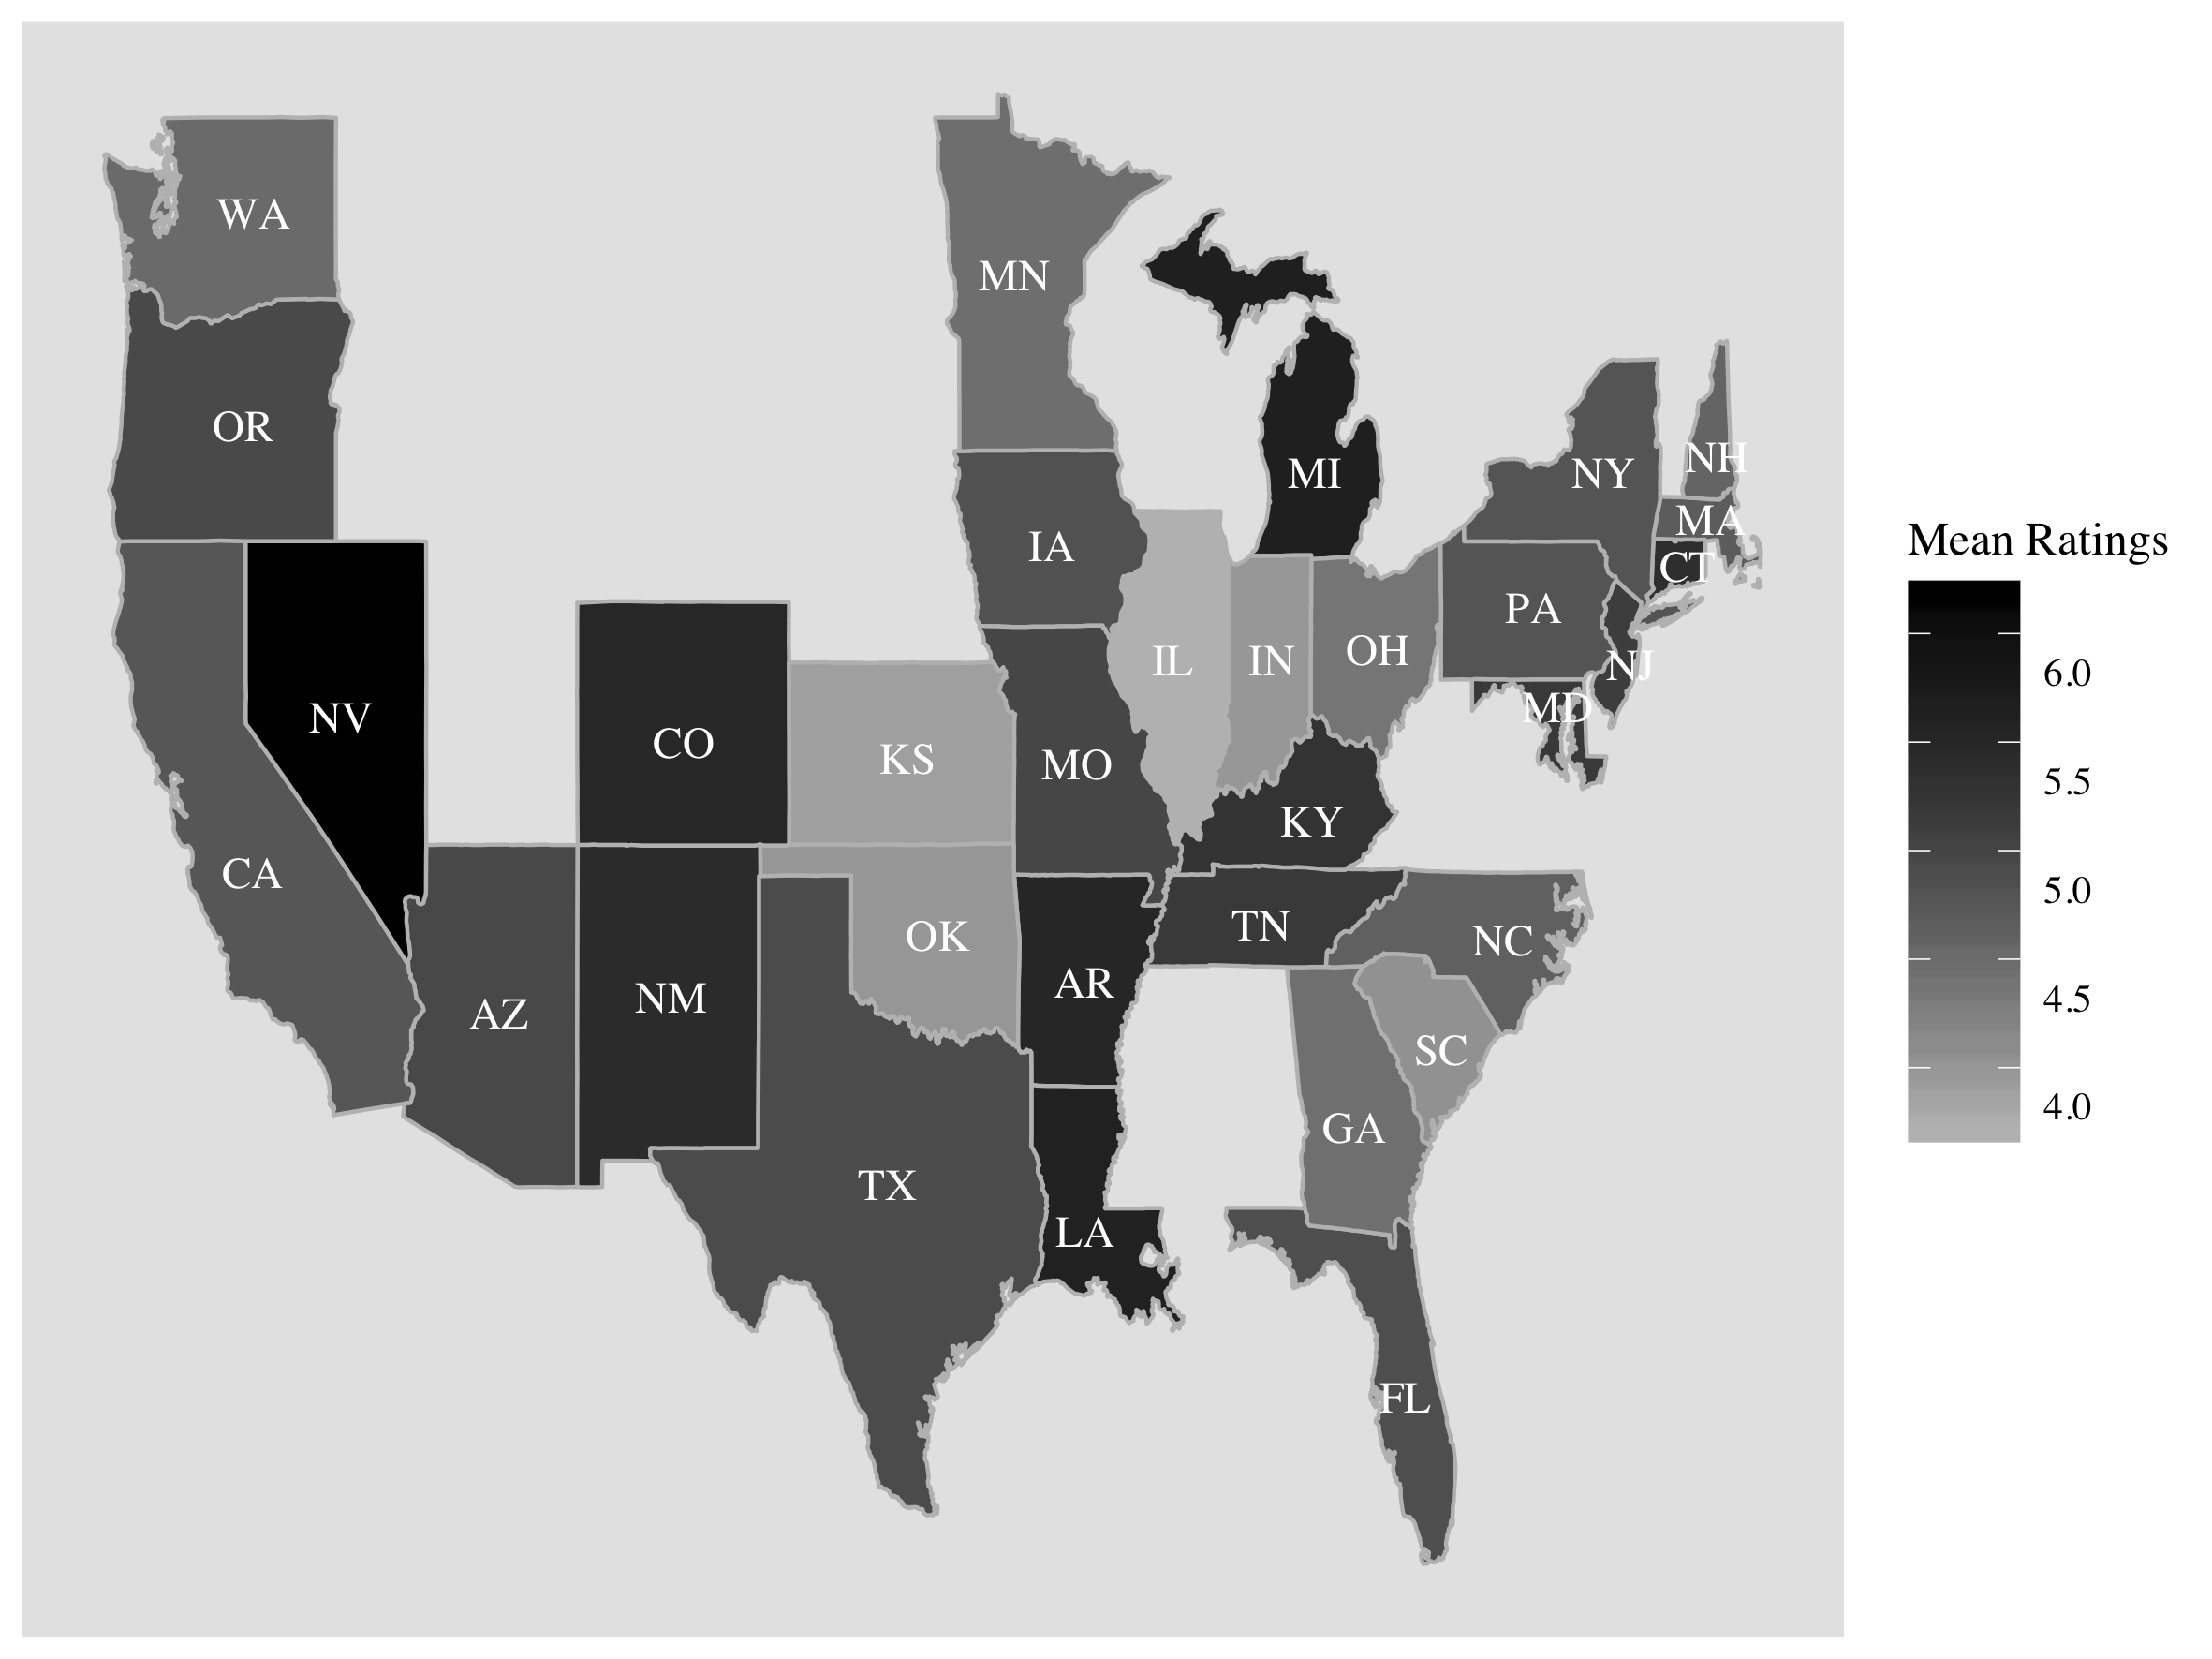
\includegraphics[width=0.9\textwidth]{figures/sup/exp1.png}
\end{frame}

\begin{frame}
\frametitle{Ratings across the US: Experiment 2}
\centering
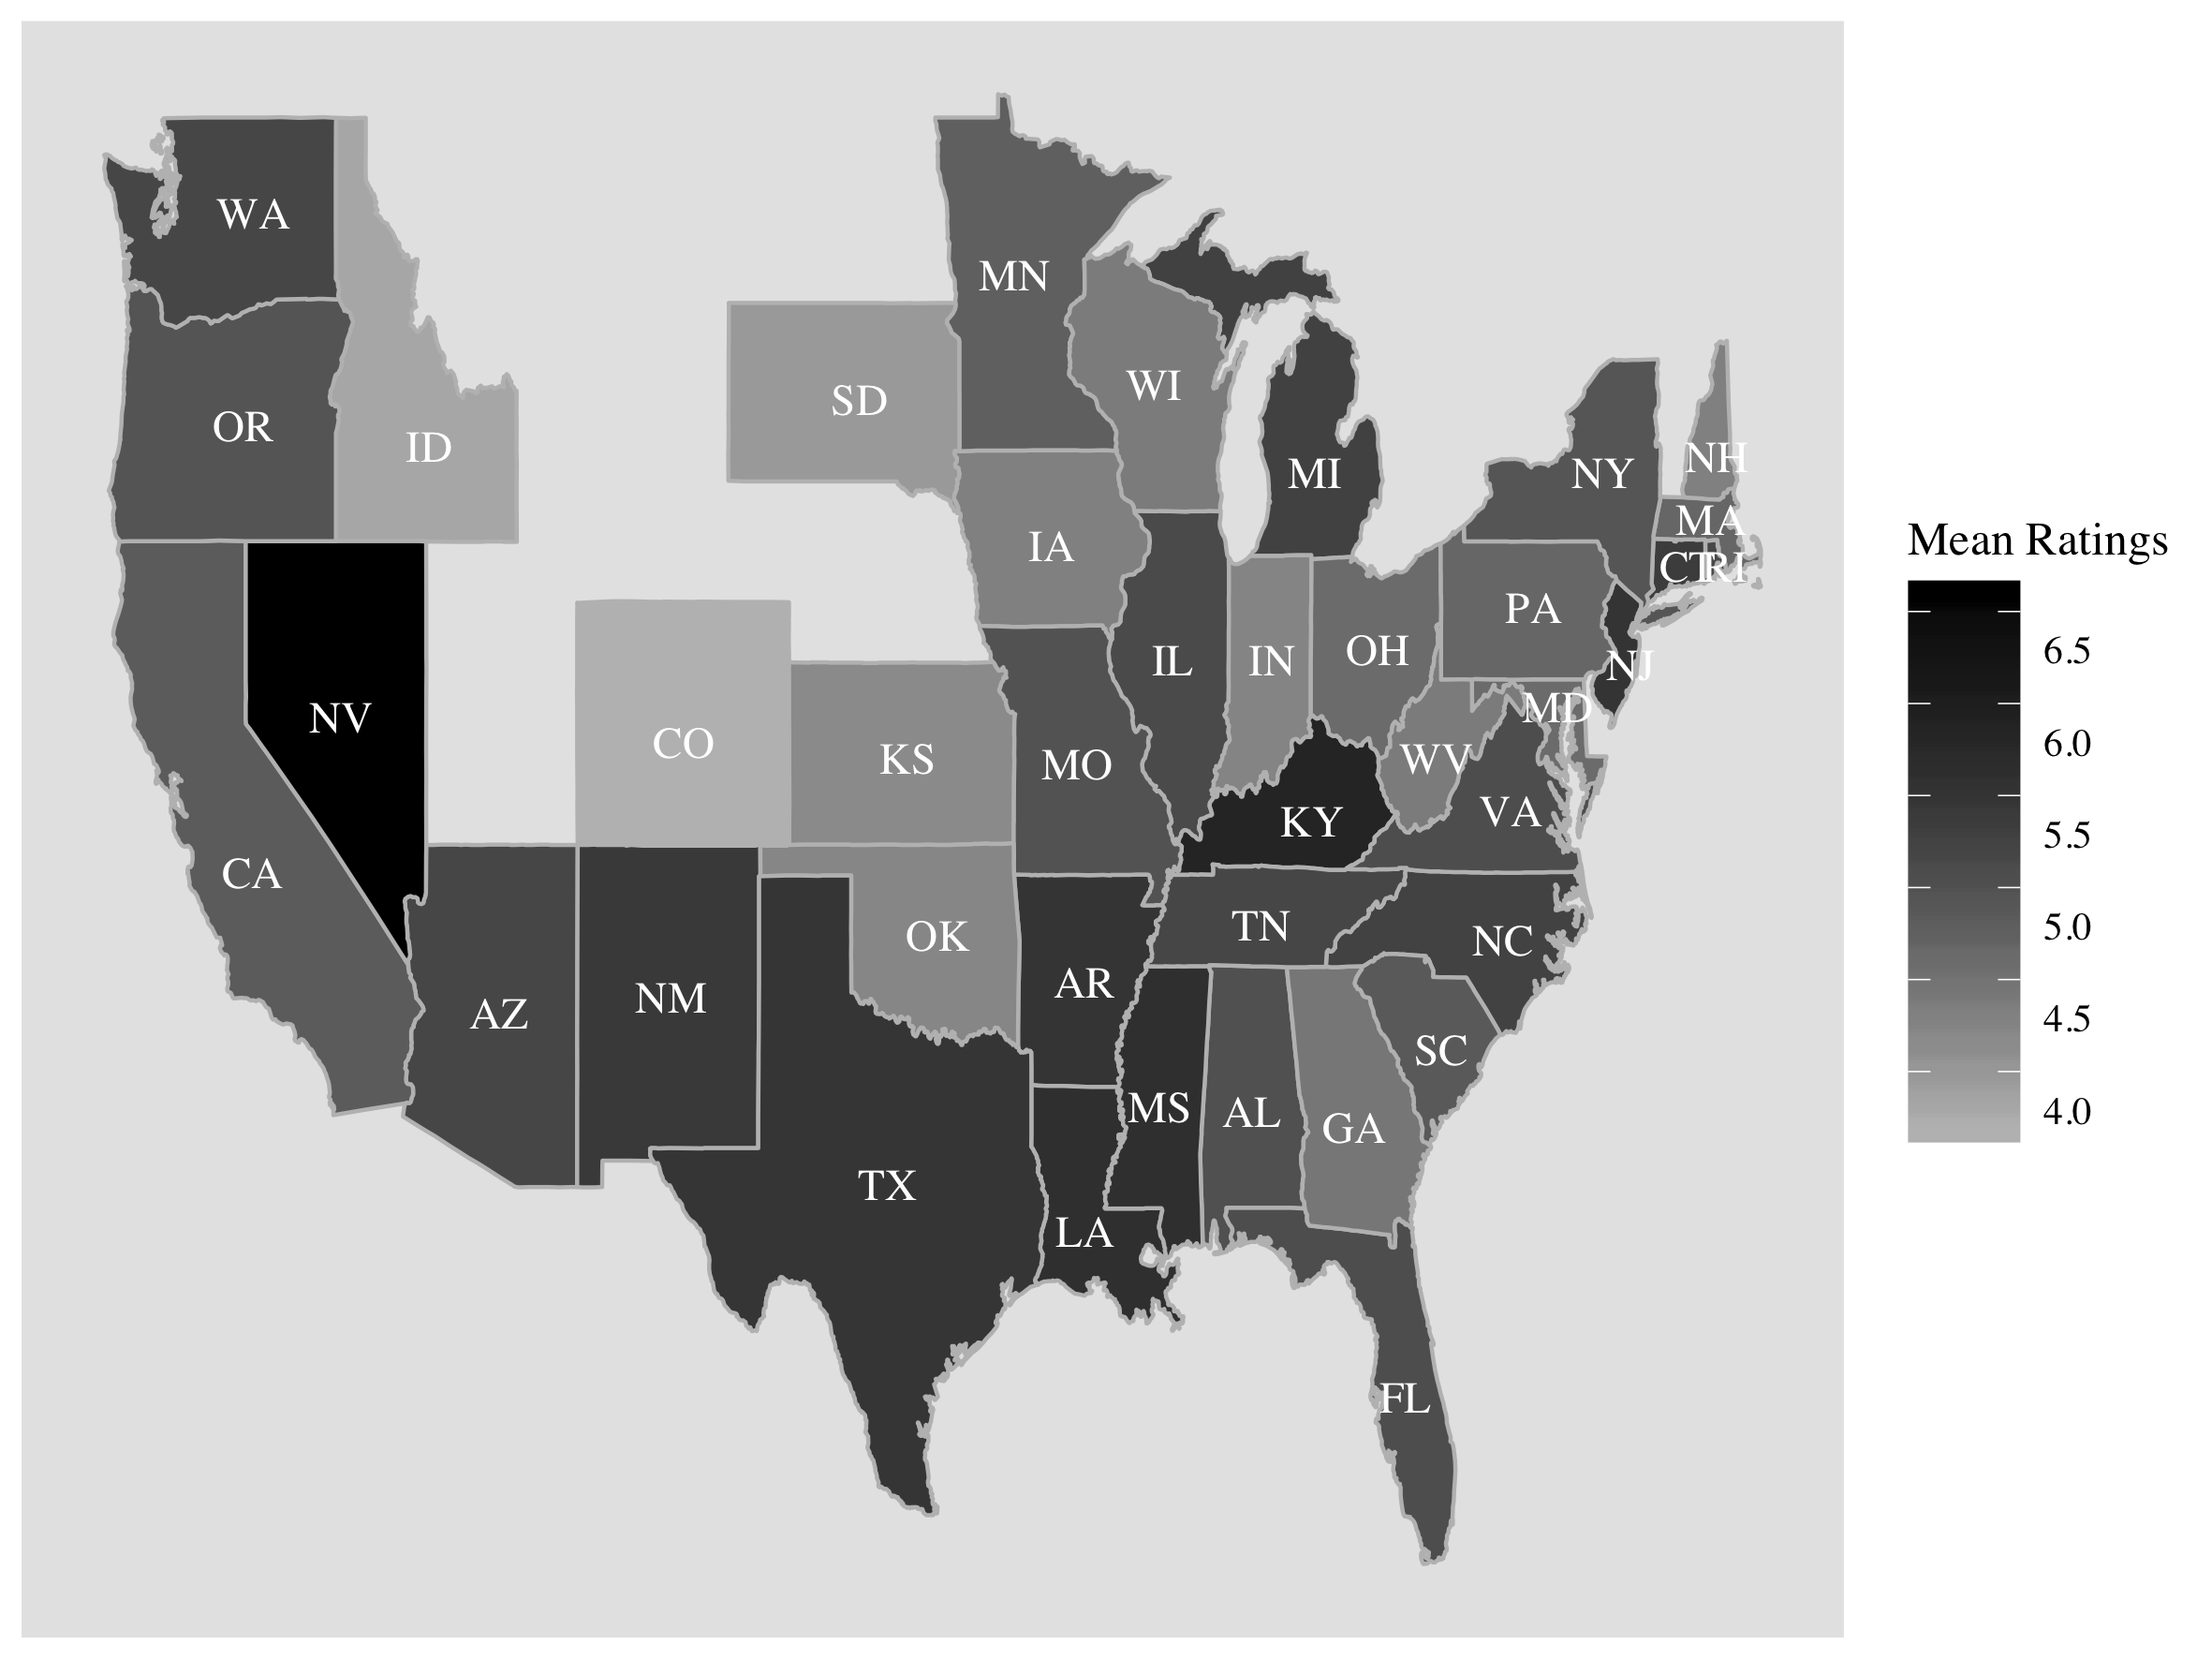
\includegraphics[width=0.9\textwidth]{figures/sup/exp2.png}

\end{frame}

\end{document}